\documentclass{sig-alternate}


\usepackage{enumitem}
\usepackage{framed}
%\usepackage[11pt]{moresize}
\usepackage{cprotect}
\usepackage{enumitem}
\usepackage{listings}
\usepackage{amstext}
\usepackage{amstext}
\usepackage{pdfpages}
\usepackage{alltt}
\usepackage{epstopdf}
\usepackage{xspace,colortbl}
\usepackage[USenglish]{babel}
\usepackage{multirow}
\usepackage[hyphens]{url}
\usepackage{subfigure}
\usepackage{graphicx}%%
\usepackage{amssymb}
\usepackage{fmtcount}
\usepackage{amsfonts}
\usepackage{xspace}
\usepackage{amsmath}
\usepackage{multirow}
\usepackage[mathscr]{eucal}
%\usepackage{psfrag}
\usepackage{colortbl}

\usepackage{amsmath,amssymb}
\usepackage[linesnumbered, ruled,vlined]{algorithm2e}

\usepackage{caption}
\usepackage{graphicx}

\usepackage{bm}
\usepackage{times}
\usepackage[nospace]{cite}
\usepackage{csquotes}
\usepackage{enumitem}

\lstset{basicstyle=\small,breaklines=true,language=Python, frame=single,escapeinside={(*}{*)}}

\usepackage{balance}

%\linespread{0.99}

\makeatletter
\def\@copyrightspace{\relax}
\makeatother


\DeclareMathOperator*{\argmin}{arg\,min}
\DeclareMathOperator*{\argmax}{arg\,max}


\begin{document}

%\setlength{\belowdisplayskip}{3pt} \setlength{\belowdisplayshortskip}{3pt}
%\setlength{\abovedisplayskip}{3pt} \setlength{\abovedisplayshortskip}{3pt}
%\setlength{\belowcaptionskip}{-10pt}
%\selectfont

\newtheorem{theorem}{Theorem}
\newtheorem{example}{Example}
\newtheorem{definition}{Definition}
\newtheorem{problem}{Problem}
\newtheorem{property}{Property}
\newtheorem{proposition}{Proposition}
\newtheorem{lemma}{Lemma}
\newtheorem{corollary}{Corollary}

\newcommand{\detectlib}{\texttt{IsoDetect}\xspace}
\newcommand{\company}{\texttt{Company X}\xspace}
\newcommand{\cond}{\textrm{pred}\xspace}
\newcommand{\dataset}{data set\xspace}
\newcommand{\datasets}{data sets\xspace}
\newcommand{\spview}{\textsf{SPView}\xspace}
\newcommand{\fjview}{\textsf{FJView}\xspace}
\newcommand{\aggview}{\textsf{AggView}\xspace}
\newcommand{\hashfunc}[1]{\textsf{hash}(#1)\xspace}
\newcommand{\hashop}{\textsf{hash}\xspace}
\newcommand{\nsc}{\textsf{NormalizedSC}\xspace}
\newcommand{\rsc}{\textsf{RawSC}\xspace}

\newcommand{\avgfunc}{\ensuremath{\texttt{avg} }\xspace}
\newcommand{\maxfunc}{\ensuremath{\texttt{max} }\xspace}
\newcommand{\minfunc}{\ensuremath{\texttt{min} }\xspace}
\newcommand{\histfunc}{\ensuremath{\texttt{histogram\_numeric} }\xspace}
\newcommand{\countfunc}{\ensuremath{\texttt{count}}\xspace}
\newcommand{\sumfunc}{\ensuremath{\texttt{sum} }\xspace}
\newcommand{\varfunc}{\ensuremath{\texttt{var} }\xspace}
\newcommand{\stdfunc}{\ensuremath{\texttt{std} }\xspace}
\newcommand{\covfunc}{\ensuremath{\texttt{cov} }\xspace}
\newcommand{\corrfunc}{\ensuremath{\texttt{corr} }\xspace}
\newcommand{\medfunc}{\ensuremath{\texttt{median} }\xspace}
\newcommand{\percfunc}{\ensuremath{\texttt{percentile} }\xspace}
\newcommand{\havingfunc}{\ensuremath{\texttt{HAVING} }\xspace}
\newcommand{\selectfunc}{\ensuremath{\texttt{select} }\xspace}
\newcommand{\ratio}{\ensuremath{\rho }\xspace}


\newcommand{\insertion}{\ensuremath{\texttt{INSERT} }\xspace}
\newcommand{\update}{\ensuremath{\texttt{UPDATE} }\xspace}
\newcommand{\delete}{\ensuremath{\texttt{DELETE} }\xspace}

\newcommand{\sysfull}{BoostClean\xspace}
\newcommand{\sys}{BoostClean\xspace}
\newcommand{\sysnospace}{BoostClean}


\newcommand{\tbl}[1]{\textsf{#1}\xspace}
\newcommand{\field}[1]{\textsf{#1}\xspace}
\newcommand{\cost}{\textrm{cost}\xspace}
\newcommand{\ans}{\textsf{ans}\xspace}
\newcommand{\dans}{\Delta\textsf{ans}\xspace}
\newcommand{\cqp}{correction query processing\xspace}
\newcommand{\Cqp}{Correction query processing\xspace}

\newcommand{\reminder}[1]{{{\textcolor{magenta}{\{\{\bf #1\}\}}}\xspace}}
\newcommand{\ewu}[1]{{{\textcolor{blue}{\{\{\bf ewu:\} #1\}}}\xspace}}
\newcommand{\mps}[1]{{{\textcolor{red}{\{\{\bf meelap:\} #1\}}}\xspace}}
\newcommand{\stitle}[1]{\vspace{0.5em}\noindent\textbf{#1}}


\definecolor{light-gray}{gray}{0.95}
\definecolor{mid-gray}{gray}{0.85}
\definecolor{green}{RGB}{0,176,80}
\definecolor{darkred}{rgb}{0.7,0.25,0.25}
\definecolor{darkgreen}{rgb}{0.15,0.55,0.15}
\definecolor{darkblue}{rgb}{0.1,0.1,0.5}
\definecolor{orange}{RGB}{237,125,49}
\definecolor{blue}{RGB}{68,114,196}
\newcommand{\blue}[1]{{\textcolor{blue}{{\bf #1}}\xspace}}
\newcommand{\orange}[1]{{\textcolor{orange}{{\bf #1}}\xspace}}



\newcommand{\specialcell}[2][c]{%
  \begin{tabular}[#1]{@{}c@{}}#2\end{tabular}}

\def\ojoin{\setbox0=\hbox{$\bowtie$}%
  \rule[-.02ex]{.25em}{.4pt}\llap{\rule[\ht0]{.25em}{.4pt}}}
\def\leftouterjoin{\mathbin{\ojoin\mkern-5.8mu\bowtie}}
\def\rightouterjoin{\mathbin{\bowtie\mkern-5.8mu\ojoin}}
\def\fullouterjoin{\mathbin{\ojoin\mkern-5.8mu\bowtie\mkern-5.8mu\ojoin}}

%\setlength{\belowcaptionskip}{-10pt}

%\newcommand{\reminder}[1] {}
\pagestyle{plain}

%\input{coverletter.tex}

%\title{ActiveClean: Progressive Data Cleaning For Convex Data Analytics}
\title{\sys: Learning an Ensemble of Data Cleaning Models to Optimize Machine Learning}


%\fontsize{9pt}{11pt}
%\selectfont


\maketitle

\begin{abstract}
As Machine Learning scales up to larger datasets, the challenges in handling dirty data during training and prediction become more significant.
Currently, it requires painstaking human effort to monitor and maintain learning pipelines to ensure that prediction accuracy does not drop due to unexpected data.
We present a system called \sys that automatically detects data errors, and selects repairs that maximally improve predictive performance of a user-defined ML model.
Since repairs are potentially ambiguous, \sys ``hedge its bets'' by using an ensemble of models trained with different repair strategies.
We describe materialization, indexing, and parallelization strategies that find this ensemble efficiently, and results suggest greater than an order-of-magnitude speedup.
\sys provides a library of dataset-independent error detectors
based on deterministic heuristics and statistical criteria. To better detect errors in categorical attributes, one of the modules in this library is a novel anomaly detector based on the Word2Vec Neural Network architecture.
We evaluated \sys on a collection of datasets from machine learning competitions, real-world data analyses, and \company, and found that statistically improvements in prediction accuracy in comparison to baseline approaches on completely unseen test data. 
We demonstrate how we can parallelize the inner-loop of the boosting operation, and on a 16-core machine, \sys achieves a 9.7x speedup.
\end{abstract}


%\pagenumbering{gobble}


\section{Introduction}\label{intro}\sloppy
The availability of data and vast cloud-based computational resources are allowing both industry and academia to build ever more sophisticated machine learning (ML) applications.
The database community has built systems that support almost every stage of the development process including featurization~\cite{keystone,zhang2014mat}, distributed model training~\cite{hellerstein2012madlib, crotty2014tupleware, feng2012towards, tensor}, and model deployment~\cite{crankshawmissing}.  
However, an often under-discussed, yet crucial, part of ML development is managing dirty data.
In the context of ML, dirty data refers to unintended or unpredictable numerical features that arise from a violation of an invariant expected by the developer (e.g., un-handled NULL values being automatically mapped to 0).
Dirty data affects both the model training and any future predictions the application might make, and numerous papers~\cite{sculley2014machine} and surveys of analysts~\cite{kandel2012, krishnan2016hilda} suggest that the effects and costs of dirty data are pervasive.

%that it takes significant effort to manually identify dirty data and design software to mitigate their effects 

\iffalse
\begin{figure}[t]
% \vspace{-5pt}
\centering
 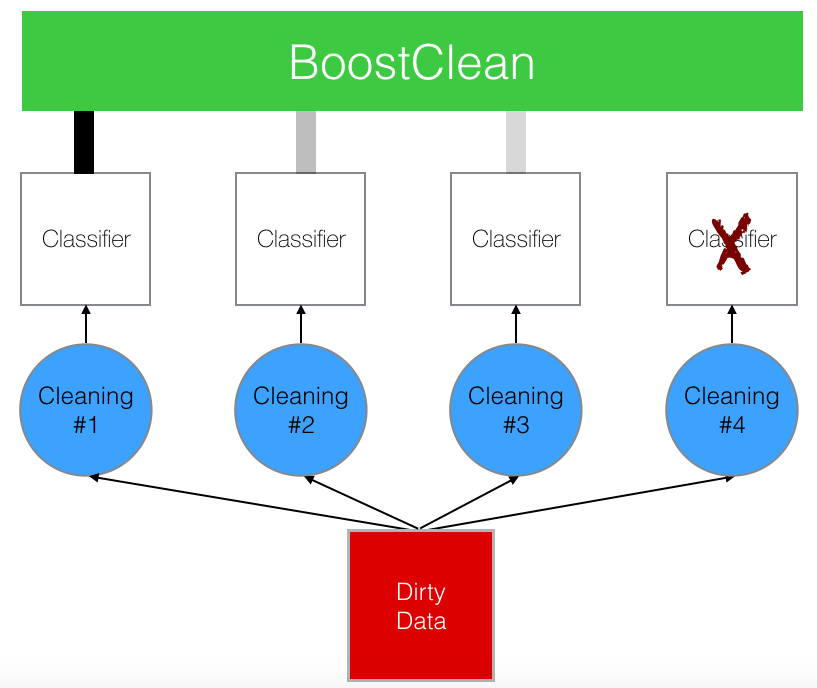
\includegraphics[width=0.8\columnwidth]{figures/teaser.png}
 \caption{ \sys is a new data cleaning system that detects errors in ML data and adaptively selects from a set of repair actions to maximize prediction accuracy. This selection problem is formulated as a statistical boosting procedure, which reweights the data to focus on model mispredictions.
 \label{fig:teaser}}
\end{figure}
\fi

As a concrete example, we are collaborating with a data science company called \company\footnote{Anonymized at the request of the company.} that ranks sales leads. The company aggregates clients' Salesforce.com data on past sales leads, integrates this data with additional information scraped from the web about the client and those leads, and trains a classification model that predicts the success of future uncontacted leads.  Because the data are acquired from a combination of manual data entry and automatically scraped web data, inconsistencies, missing data, and incorrect values are a significant problem.  For instance, a typical error is the inconsistent representation of missing values (e.g., ``-999'', ``EMPTY'' or ``none'' may be used depending on the sales representative).  If the featurization code does not recognize and address these errors, it can lead to biases that degrade the quality of the model. For example, the data scientist may impute a default mean value for all blank attributes but miss the code ``-999'', which is then interpreted as a semantic value. 
At the company, detecting and repairing errors takes roughly 1 week of human manual work per dataset. 
Furthermore, the company has heterogeneous data and this effort will have to be spent each time a new dataset is used.

Surveys suggest that this company's data cleaning challenges are not unique and are prevalent in many industrial ML pipelines~\cite{krishnan2016hilda}.  
Software Engineers write custom conditional cleaning scripts that are a combination of a {\it detector}, which are a collection of Boolean functions that specify a subset of records that are dirty, and {\it repair} functions that transform or delete those records.  It is not enough to write these scripts once, as the predictive nature of ML applications means that they are continuously encountering new, unseen data.
Software Engineers must constantly monitor and maintain the data processing pipeline to account for unexpected changes to the input data~\cite{sculley2014machine, DBLP:conf/sigmod/KrishnanFGWW16}.
To reduce this burden, we present a new system, called \sys, that explores automating error detection and repairs for ML applications.   
Our focus is on automating routine operations (primarily domain value violations), and leaving more complex scenarios, such as entity resolution, to custom scripts.
This can ensure that deployed models maintain high accuracy even in the presence of some dirty data, and engineers are only needed to address drastic changes to the input data. 

Data cleaning for such data science applications presents additional structure that we can exploit in \sys.
First, we assume that downstream predictive model is known and we can query this model.
Recent work suggests that data cleaning can made significantly more efficient by prioritizing records to clean based on the  desired downstream analysis~\cite{altwaijry2015query, DBLP:conf/sigmod/BergmanMNT15, DBLP:journals/pvldb/KrishnanWWFG16}.
Next, in ML applications, test data is often available (e.g., the results of following a sales lead) and can be used as a mechanism to evaluate the results of data cleaning.  
It is often a reasonable assumption that in the test data the prediction labels are clean, since they often represent directly observed phenomena such as (e.g., purchased/not purchased).
We can leverage the test data to evaluate the impact of  a given cleaning operation on whether it will improve or hurt a model's prediction accuracy.
The key challenge will be an efficient search over the space of conditional data cleaning scripts (detectors and repairs), while ensuring that the model does not overfit~\cite{DBLP:journals/pvldb/KrishnanWWFG16,krishnan2016hilda}.   

Our primary observation is that a given conditional cleaning script can be interpreted as generating a new set of features--thereby generating a new model trained on those features. 
We can view the process of selecting the best sequence of cleaning operations as an ensembling problem, i.e., selecting the best collection models that collectively estimate a label. 
Although there are many possible algorithms~\cite{dietterich2000ensemble}, we use a technique called Boosting~\cite{freund1995desicion}, which composes a set of weak learners into a strong learner.  
First, unlike methods that are specific to certain classes of models (e.g., linear models, differentiable models), boosting can be applied to black-box models. 
Second, it takes interactions and correlations between the different data cleaning models into account by incrementally selecting ``orthogonal'' compositions.


% is similar cleaning operations can be viewed as collections of feature extraction operations, and consequently, automated feature selection techniques can be adopted to the data cleaning setting.  For example, consider a cleaning operation that fills an empty attribute value with a default value.  The default value may be the most common value in the dataset, the mean value, or even a random attribute value in the dataset; every default value setting corresponds to a specific {\it instance} of a cleaning operation, and can be viewed as a separate feature extraction function.  Thus the goal is to select a sequence of cleaning operation instances that maximizes the downstream model's test accuracy.


\sys takes as input a relational table, a library of detector functions $\mathcal{D}$ that generate (possibly incorrect) predicates that match candidate dirty records, a library of repair functions $\mathcal{F}$ that transform or delete a record, and a user-specified classifier training procedure \texttt{train()}.
\sys has two key components: an automatic error detector to determine subsets of records that are dirty, and a repair selector to select repair actions for those dirty records using boosting.
For the error detector, we designed a modular error detector architecture based on Isolation Forests~\cite{liu2008isolation}.
Isolation Forests essentially apply axis-aligned random cuts to a dataset to measure how easy it is to separate a record from the rest of the distribution.
We combine this architecture with numerical and textual featurizers to detect errors in a dataset.
One of these featurizers is a novel adaptation of \textsf{word2vec} neural network architecture for detecting multi-attribute errors.
The neural network learns to predict the co-occurrence of attributes in a record and can be used to generate a featurization for anomaly detection.
Once errors are detected (represented as a predicate $p_i$), \sys uses boosting to generate a sequence of conditional repairs $(p_i, r_i)$,  $r_i$ is the repair function to be applied on the records that match predicate $p_i$.

\vspace{0.25em}\noindent\textbf{Scope of this paper: } This paper focuses on supervised classification models (both single and multi-class), and single-node model training.
We also primarily consider domain integrity constraint violations where attribute values have to conform to a specified domain or pattern.

\subsubsection*{Contributions}

\vspace{0.25em}\noindent\textbf{Boosting: } We present a new data cleaning system based on statistical boosting that finds the best ensemble of operations from a library of operations to maximize the predictive performance of a downstream model. We evaluated \sys on a collection of datasets from machine learning competitions, real-world data analyses, and \company, and found that statistically improvements in prediction accuracy in comparison to baseline approaches on completely unseen test data. 

\vspace{0.5em}\noindent\textbf{Error Detection: } We build an optimized library of data cleaning operations based on deterministic rules and statistical criteria from which \sys selects. To better detect errors in categorical attributes, one of the modules in this library is an anomaly detector based on the Word2Vec Neural Network architecture. On 8 of the experimental datasets, the library achieves a detection accuracy of 81\% of all of the errors found by hand-written rules. We also show that this is on average 40\% more accurate than applying statistical outlier detection to only the quantitative attributes.

\vspace{0.5em}\noindent\textbf{Optimizations: } We demonstrate how we can parallelize the inner-loop of the boosting operation, and on a 16-core machine \sys achieves a 9.7x speedup for the repair selection step. Similarly, we show that building an index can speed up operator selection time by more than 10x for a 1.5GB dataset.






\iffalse
The problem of dirty training data in ML is subtle as most learning algorithms are robust to statistical noise.
However, un-modeled systematic biases in the training data can still adversely affect the results~\cite{DBLP:journals/pvldb/KrishnanWWFG16, DBLP:conf/case/MahlerKLSMKPWFAG14, xiaofeature}.
The way that the developer chooses to address corruption will have a significant impact on the performance of the ML application.
Consider a music recommender system where a recent software update causes songs longer than 5 minutes to have ``NULL'' ratings.
If the ML developer treats a NULL rating as ``0 stars'', those songs may never get recommended.
To avoid this bias, it may be more prudent to discard those ratings or impute a default  value (e.g., mean over all previous non-NULL ratings).

To setup the abstract search problem, we are given a dataset $R$, a library of data cleaning operations $\mathcal{L}=\{l_1,...,l_k\}$, a user-specified model training program which returns a classifier, and an oracle that evaluates the prediction accuracy of the classifier (e.g., a ground truth clean test dataset).
Our objective is to find a classifier that maximizes prediction accuracy by applying compositions of operators in our library to $R$ and training on the resulting dataset.
While this problem is inherently combinatorial, the key insight is to model the hypothesis testing procedure as a form of adaptive statistical boosting. 
\fi




%The datasets are inconsistent in the way they represent missing information (e.g., some numerical fields left blank, some fields with a placeholder value of ``-999''). 
%Featurization code that does not recognize that a blank attribute value is semantically equivalent to a ``-999'' attribute value can lead to biases--for example, the data scientist may impute a sensible default mean value for all of the blank attributes but treat the ``-999'' as the given value.

\if{0}
Clearly, some level of automation in detecting and handling erroneous data can reduce the burden on data scientists.
Automated rule-based data repair is a well-studied field~\cite{DBLP:conf/sigmod/ChuIKW16}, but the ML setting presents additional challenges and structure that are important to understand.
In ML, incoming records are, in a sense, both data (during training) and queries (during prediction).
This provides additional degrees-of-freedom in handling dirty data.
For example, when asked to predict a label for a dirty example, one may want to return a ``fail-safe'' prediction instead of cleaning it first and then asking for a prediction.
Second, ML applications often have a way of measuring prediction accuracy.
Labels often represent directly observed user-behavior (e.g., sale vs. no sale, whether the user clicked a link etc.), and thus, are relatively consistent over the lifetime of an application.
On the other hand, the features used to predict the labels may be integrated from a variety of different company databases and susceptible to inconsistencies and change.
With this in mind, we present \sys, a new data cleaning system that detects errors in ML data and uses knowledge of the labels to adaptively select from a set of repair actions to maximize prediction accuracy.
\fi

\section{Background}
This section motivates \sys in relation to prior work.
Using the pilot study as inspiration, we use a simplified running example to present the system and notation:
\begin{example}[Lead Prediction]\sloppy\label{ex:lead}
Past clients are stored in a relational database:
\[
R(id, name, num\_emp, industry, region, successful)
\]
where $name$ is the company name, $num\_emp$ is the number of employees in the company, $industry$ is a categorical attribute that describes the industry segment, $region$ is a code indicating the region of the country the business is headquartered, and $is\_successful$ is a Boolean describing whether the company purchased the product.
\end{example}

\begin{figure}[t]
% \vspace{-5pt}
\centering
 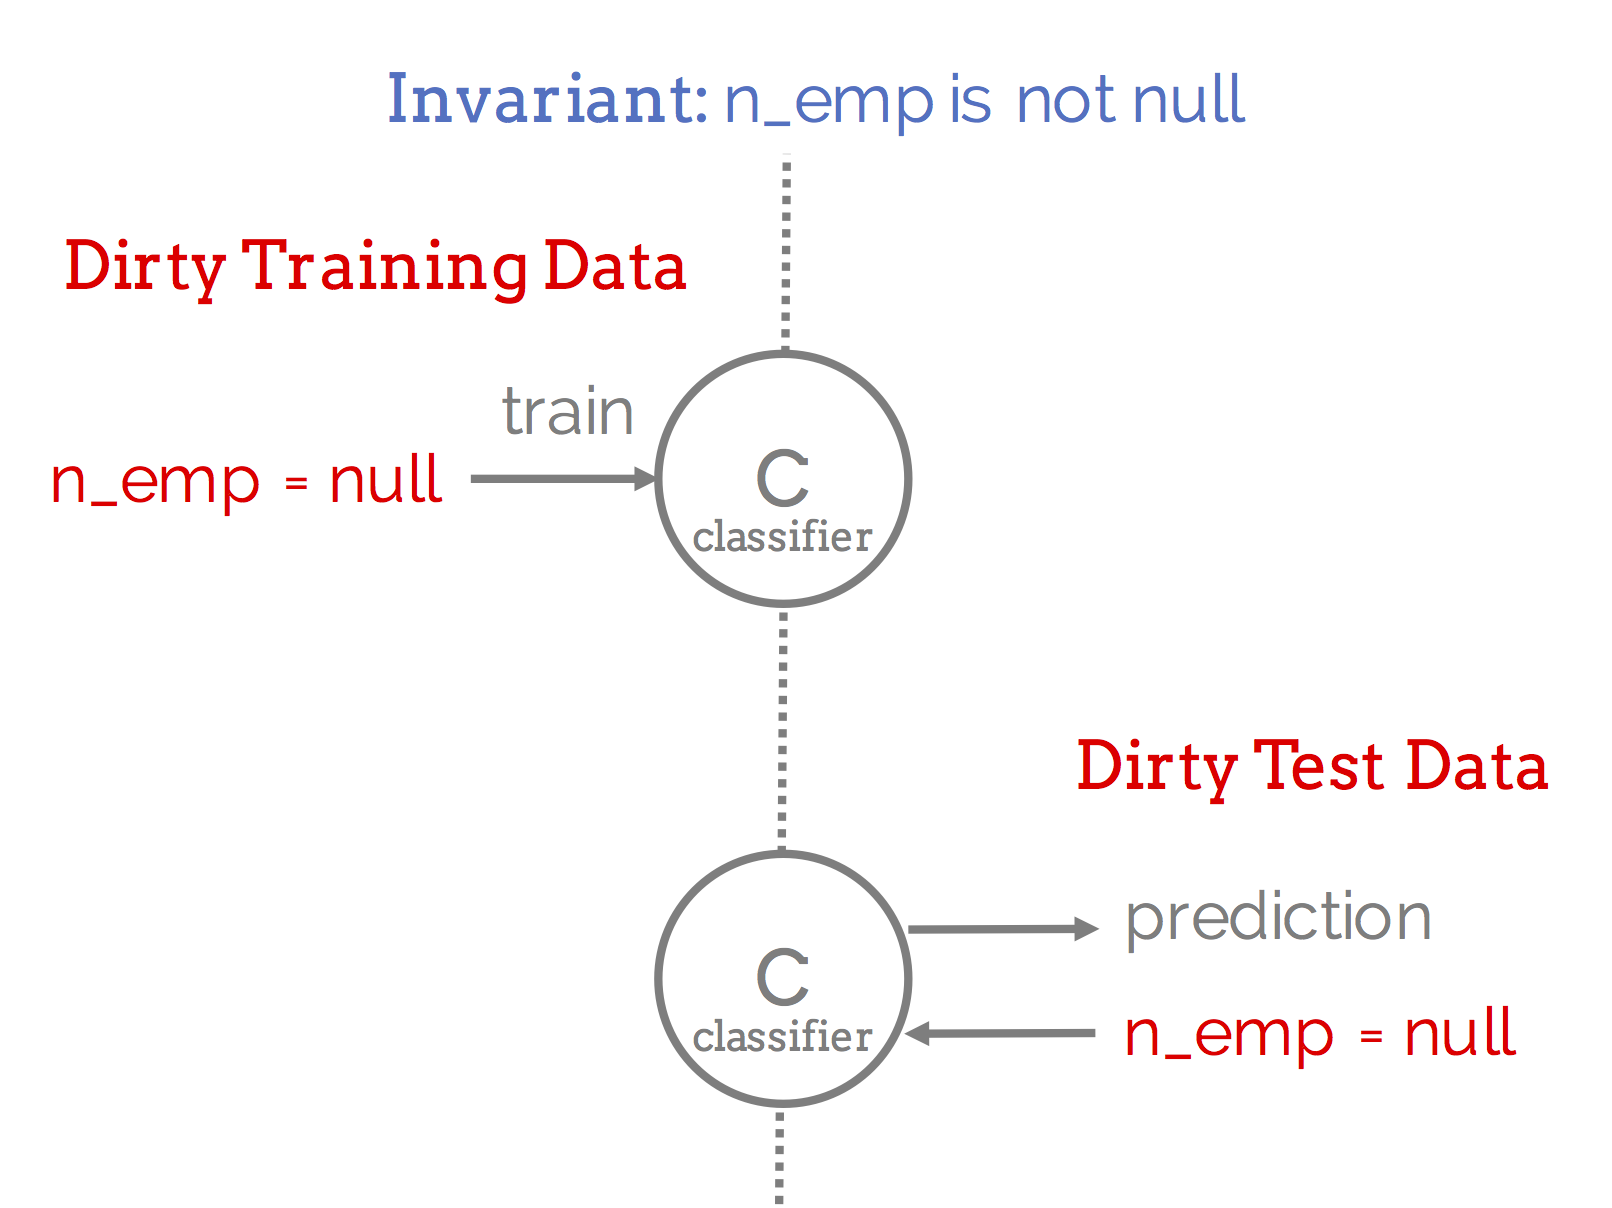
\includegraphics[width=\columnwidth]{figures/training_and_pred_errors.png}
 \caption{The above example uses the invariant that the number of employees is greater than $0$.  Training errors are violations of the invariant in the training dataset (top row). Prediction errors are invariant violations in the test data during prediction. \sys is a tool to {\it detect} both types of errors and generate a corrective {\it repair} action.
 \label{fig:error}}
\end{figure}

\subsection{Machine Learning and Dirty Data}
It is important to highlight a number of points when considering data cleaning in the machine learning context.
First, machine learning models are often robust to statistical noise and inherent variations in the dataset.  For this reason, our focus is not to reduce random noise; instead, our focus is to identify and address systematic errors due to invariant violations that lead to unforeseen biases in the model.  
For example, records with a positive classification label are more likely to have NULL values in the training set.
Figure \ref{fig:error} illustrates two examples of how this can affect a model.
Second, while the notion of invariants is similar to integrity constraints in traditional relational data cleaning, the way that repairs are evaluated differ.  Relational data cleaning focuses on identifying a minimal set of repairs that resolve a set of constraint violations.  On the other hand, our goal is to improve the the downstream model test prediction accuracy.  These goals are not necessarily aligned, and by ignoring the downstream model, it is possible that traditional cleaning techniques perform cleaning operations that degrade the model accuracy.

\subsection{Existing Approaches}
\sys brings together generic, dataset-independent error detection with automatically learned repair strategies for ML applications.
We review how baseline techniques proposed in prior work that could apply to this problem.

\vspace{0.5em}

\noindent\textbf{Rule-based Repair: } 
In the running example, suppose some of the values for $num\_emp$ are NULL and we want to train a classifier to predict $is\_successful$.
We would define a domain integrity constraint $num\_emp \ne~NULL$, and then propose a set of repairs to satisfy this constraint.
With no other information, this rule-based approach could in principle impute any non-null value from the domain to create a logically consistent relation.
To avoid this problem, we can adopt an approach like~\cite{prokoshyna2015combining} and select the imputations that minimize the statistical distance of the updated relation to an ideal distribution for the attribute, for example, an ideal power-law distribution.
This would impute values in such a way that $num\_emp$ matched a Zipfian distribution.

When we train a classifier after applying such a technique, counter-intuitive effects can occur.  
The data cleaning operation may break important correlations in the data and may introduce biases into the training data not present in test conditions. 
Consider the degenerate case where $num\_emp = NULL$ is perfectly correlated with one of the prediction classes--in this case, it may be better to NOT clean the data!
While more sophisticated statistical imputation techniques exist~\cite{schafer1998multiple}, they all have the same fundamental problem that the value imputation is divorced from the downstream classifier's predictive accuracy. 
We see this problem in our experiments (Section~\ref{exp:comp}), where on some datasets imputing the most frequent value leads to a more accurate downstream classifier than imputing to minimize the difference from an ideal distribution.

\vspace{0.5em}\noindent\textbf{Statistical Detection: } Rule-based techniques are dependent on the analyst defining the invariants. Defining such invariants can be challenging if the analyst is working with a new dataset, if she cannot anticipate how future data might look, or if the number of datasets is too large (e.g., in a data lake setting).
There is a well-established line of literature on statistical anomaly detection~\cite{hellerstein2008quantitative}, and for the most part, these techniques are generic and dataset independent (up-to hyperparameters). Typically, such approaches identify \emph{outlier} records outside of some normal range of variance. However, the problem is that not all dirty data look like outliers. In the running example, there could truly be companies where $num\_emp = 0$. It has been shown that statistical anomaly detection techniques miss obvious errors in heterogeneous datasets that contain a mixture numerical, categorical, and string-valued attributes~\cite{DBLP:journals/pvldb/AbedjanCDFIOPST16}.

Abedjan et al. recently evaluated a wide range of error detection techniques on 5 proprietary real-world datasets~\cite{DBLP:journals/pvldb/AbedjanCDFIOPST16}.  They found that the errors in 3 of the datasets were dominated by missing cell values; 1 dataset contained functional dependency violations due to erroneous numerical attribute values, and only 1 dataset require complex user-specified denial constraints~\cite{chu2013discovering} to identify the errors.  These findings suggest that, in 4 of the 5 datasets, a significant portion of data errors can be classified as {\it domain integrity errors}, wherein a cell contains a value outside of its domain of permissible values.

\stitle{Towards Automated Cleaning:} We believe this highlights the potential value of automated cleaning systems such as \sys to identify the bulk of common-case errors, so that developers may focus on the specialized, domain-specific errors.  The prevalence of {\it domain integrity errors} suggests that a pre-defined set of featurizers and detector generators can be sufficient to detect these errors.  In fact, on 8 of our experimental datasets, \sys using our pre-populated detector library achieves a detection accuracy of 81\% of all of the errors found by hand-written rules.

Therefore, we need a mix of statistical rules and logic rules to determine errors.
We explore to what extent we can derive these rules from data for routine errors. 
We surveyed 8 ML datasets used in Kaggle competitions and benchmarks in the UCI ML repository, and found that a majority of the non-statistical errors could be detected as \emph{domain integrity constraints}, i.e., disallowed values in single columns.
We apply a combination of heuristic checks for missing values and data type errors, and a neural network based error detector that identifies attribute values not likely to co-occur in the same record.

\iffalse
\subsection{Solution Overview}
There does not exist one single error detector or repair action that dominates, so which ones should an analyst choose? 
\sys models this problem as a boosting problem.
Rather than thinking of each of detector and repair pair as a data transformation, it thinks of each as generating a new ``classifier'' that provides some additional information about the label.
The problem of selecting the top data pairs is equivalent to ensembling a subset of the classifiers as best as possible.
We choose a boosting framework to represent this problem due to the relatively minimal assumptions about the structure and implementation details of the user-specified classifier.
To construct the underlying library of cleaning operations we surveyed datasets on Kaggle and the UCI repository and built a library of data cleaning operations that supported common data cleaning tasks across the datasets.
\fi
\section{Problem Statement}
We now present the formal problem statement along with our assumptions.

\subsection{Data}
\sys takes as input a dirty training dataset $(X_{train}, Y_{train})$ where both the features $X_{train}$ and labels $Y_{train}$ may have errors, as well as a test dataset $(X_{test}, Y_{test})$ where the features may contain errors however the labels $Y_{test}$ are correct.  Although the training labels may contain errors, the test labels must be clean in order to ensure an unbiased measure of accuracy that is not affected by data cleaning operations.  Such labels may be collected as part of a gold standard dataset~\cite{marcus2015crowdsourced} or by cross-referencing the data with other sources~\cite{li2012truth}.  
Labels often represent directly observed phenomena such as (e.g., purchased/not purchased), while features are integrated from multiple disparate sources and subject to fequent change.
Let a record $r_i = (x_i,y_i) \in (X_{train},Y_{train})$ denote the features along with its corresponding (possibly null) label, and $r_i.y$ denote the label for the record.    Furthermore, the features may be categorical, or string-valued, in addition to numerical.

\begin{example}[Notation]
In Example~\ref{ex:lead}, the attributes $name$, $n\_emp$, $industry$, and $region$ define the schema of $X_{train,test}$, and the attribute $successful$ corresponds to the labels $Y_{train,test}$.
\end{example}

Let a classifier $C(r_i) = r_i'$ be a function that takes as input a record $r_i$ and sets $r_i.y$ to the predicted label value.
A classifier predicts $(x_i, y_i) \in (X_{test}, Y_{test})$ correctly if  $C((x_i, null)).y = y_i$.  $C$'s test accuracy is defined as the fraction of correctly predicted test records:
\[
acc(C) = \frac{|\{\forall x,y \in (X_{test}, X_{test})~:~ C((x, null)).y = y\}|}{|Y_{test}|}
\]
To generate a classifier, the user provides \textsf{train}($X_{train}, Y_{train}$) that return a classifier $C$. We model \textsf{train}($\cdot$) as a black-box and assume that the function interally performs any necessary featurization.

\begin{example}[Classification]\sloppy
The classifier $C$ can be a support vector machine predicting whether $successful = true$ based on a feature vector derived from
$name$, $n\_emp$, $industry$, and $region$.
\end{example}

\subsection{Detection and Repair Libraries}
We assume that the user provides a library of detector generators $\mathcal{D} = \{d_1,\cdots\}$ and a repair library $\mathcal{F} = \{f_1,\cdots\}$.  \sys uses $\mathcal{D}$ to generate predicates that identify candidate dirty records, and selects the appropriate repair functions in $\mathcal{F}$ to those records.  

\subsubsection{Detection Generators and Predicates}
We define a predicate $p_i$ as a Boolean expression over an input record that returns the set of referenced attributes if it evaluates to $true$ and an empty set otherwise.  Based on this definition, we say that $r$ is a candidate dirty record if $p_i(r) \ne \emptyset$. For instance, $p_i(r) = r.n\_emp \le 0$ is an example of the former: if a company record contains $0$ employees, then the predicate will return $\{n\_emp\}$.  We extend this simple predicate rule in three ways: 

First, predicate expressions may also reference combinations of attributes.  For instance, if we knew that there are no oil and natural gas companies in the northwest, the predicate $p_i(r) =  (r.region == USNW \wedge r.industry \in ('OIL','NG'))$ would return $\{region, industry\}$ if such a company were detected.

Second, predicates may apply transformation functions over the input data.  For instance, the following predicate first featurizes the record using a function $g$, and applies a threshold to the first element of the feature vector: $p_i(r) = g(r)[0] > 10$.  

Third, predicate expressions may contain aggregate expressions that are computed over all records in the training dataset $X_{train}$.  For instance, the following predicate performs Quantitative Error Detection~\cite{hellerstein2008quantitative} by checking whether the record's $n\_emp$ value is further than $5$ standard deviations of the mean: 
$$p_i(r) = |r.n\_emp - avg(r.n\_emp)| > 5\times stddev(r.n\_emp)$$
Finally, a detector generator $d_i$ is simply a function that takes the full training set as input and returns a predicate $p_i$. 

\subsubsection{Repair Functions}
Each repair function $f_i \in \mathcal{F}$ is a function that takes a record as input and modifies the record's attributes.  We consider two types of repairs:  {\it data repairs} are applied to the training data prior to running the training procedure, while {\it prediction repairs} modify the label of the records {\it after} the classifier makes a prediction.   

{\it Data repairs} modify the values of a training record in response to a detected error (due to a predicate).  These repair functions are free to modify the record's features, label, or simply delete the record from the training dataset.  

{\it Prediction repairs}, on the other hand, take as input the non-transformed record along with the classifier prediction, and replaces the prediction with a default value .  This is useful when the input record is too corrupted to provide a reliable prediction.  For instance, the the NFL play-by-play dataset describe in Section~\ref{s:experiments}, some input records contain almost all null attributes and it is more accurate to default the prediction to the most frequent label rather than attempting a repair.

Note that this section formalizes an API for these operations and subsequent sections provide one instantiation of this library.

\subsubsection{Conditional Repairs}
\sys applies repair functions to specific sets of records through the use of {\it conditional repairs}.  A conditional repair $l_k = (p_k, f_k)$ is a tuple where $p_k = d_i(X_{train}, Y_{train})$ is the output of a detector generator and $f_k \in \mathcal{F}$ is a repair function.
A conditional repair is compiled into generation procedure that returns a repair function; the repair function takes as input a possibly cleaned record $r$, along with its original uncleaned version $r_{orig}$:
{\small\begin{verbatim}
    def generate_repair(p, f):
      def repair(r, r_orig):
        if p(r): r = f(r)   
        return r 
      return apply
\end{verbatim}}

\begin{example}[Value Canonicalization]\sloppy
The following script canonicalizes different representations for Western United States:
{\small\begin{verbatim}
    def repair(r, r_orig):
      if r.region in ('USWest', 'USWESTERN'):
        r.region = 'USW'
      return r
\end{verbatim}}
\end{example}

\vspace{0.25em}
\begin{example}[Default Prediction]\sloppy
The following script represents a conditional prediction repair that 
predicts $false$ if the company name is missing.  Note that the predicate is applied on the original non-cleaned record, however the classifier takes as input the cleaned version.
{\small\begin{verbatim}
    def repair(r, r_orig):
      if r_orig.name == None:
        r.y = False
        return r
      return C(r)
\end{verbatim}}
\end{example}

\noindent Finally, let $\mathcal{L} = (l_1,\cdots,l_n)$ be a sequence of conditional data and prediction repairs that \sys generates. To apply the repairs, \sys first partitions the $\mathcal{L}$ into two subsequences $\mathcal{L}^d = (l_i \in \mathcal{L} | l_i$ is data repair$)$ and $\mathcal{L}^p = (l_i \in \mathcal{L} | l_i$ is prediction repair$)$.  During the training phase, we apply the data repairs in sequence over the training dataset prior to training the classifier:
\begin{align}
(X'_{train}, Y'_{train}) = \{\mathcal{L}^d(r, r) | r \in (X_{train}, Y_{train}) \}\\
C = train((X'_{train}, Y'_{train})\\
\mathcal{L}^d(r, r) = l_k(l_{k-1}(\cdots l_1(r, r), r) r) | l_i \in \mathcal{L}^d
\end{align}

Finally, \sys constructs the final classifier $C_{\mathcal{L}}$ by combining the prediction repairs $\mathcal{L}^p$ with the trained classifier $C$.  It first identifies the last prediction repair $l^* \in \mathcal{L}^p$ whose predicate matches the test record.  
$$l^* = \argmax_{l_i \in \mathcal{L}^p \wedge l_i(r) = true} i$$
If no such prediction repair is found, \sys  returns the classifier prediction on the cleaned record, otherwise it applies $l^*$:
$$C_{\mathcal{L}}(r) = \begin{cases}
    C(\mathcal{L}^d(r, r))& \text{if } l^*\textrm{\ not\ found}\\
    l^*(\mathcal{L}^d(r, r), r) & \text{otherwise}
\end{cases}$$



\subsection{Problem Statement}
This problem formulation makes several simplifying assumptions.  
First, each record in a relation corresponds to a single example (features and labels), and the analyst wants to learn a classifier that predicts labels from features; second, the relation adheres to a schema (though it may be highly sparse); and third, that the labels of the test data are clean since \sys relies on uncorrupted labels to estimate the model's accuracy.
Given these assumptions, we define the repair selection problem:

\begin{problem}[\sys Repair Selection]\sloppy
Given $(X_{train}, Y_{train})$, $(X_{test}, Y_{test})$, a library of detector generators $\mathcal{D}$ and of repair functions $\mathcal{F}$, and a training procedure $train$, identify the optimal sequence $\mathcal{L}^*$ of $B$ conditional repairs such that the resulting classifier $C_{L^*}$  maximizes prediction accuracy on $(X_{test}, Y_{test})$:
$$\mathcal{L}^* = \argmax_{L \in \mathcal{D}\times\mathcal{F}} acc(C_L)$$
\end{problem}

Greedy solutions that select the top $B$ individual condition repairs will often fail since they might select highly correlated repairs (e.g., imputing a missing value with the mean, and the median).
Instead, it is desirable for an approach to take the mispredictions from previous conditional repairs into account.  This is the reason we applied a boosting-based approach towards selecting conditional repairs, described in the next section~\cite{schapire2003boosting}.

\begin{figure}\centering
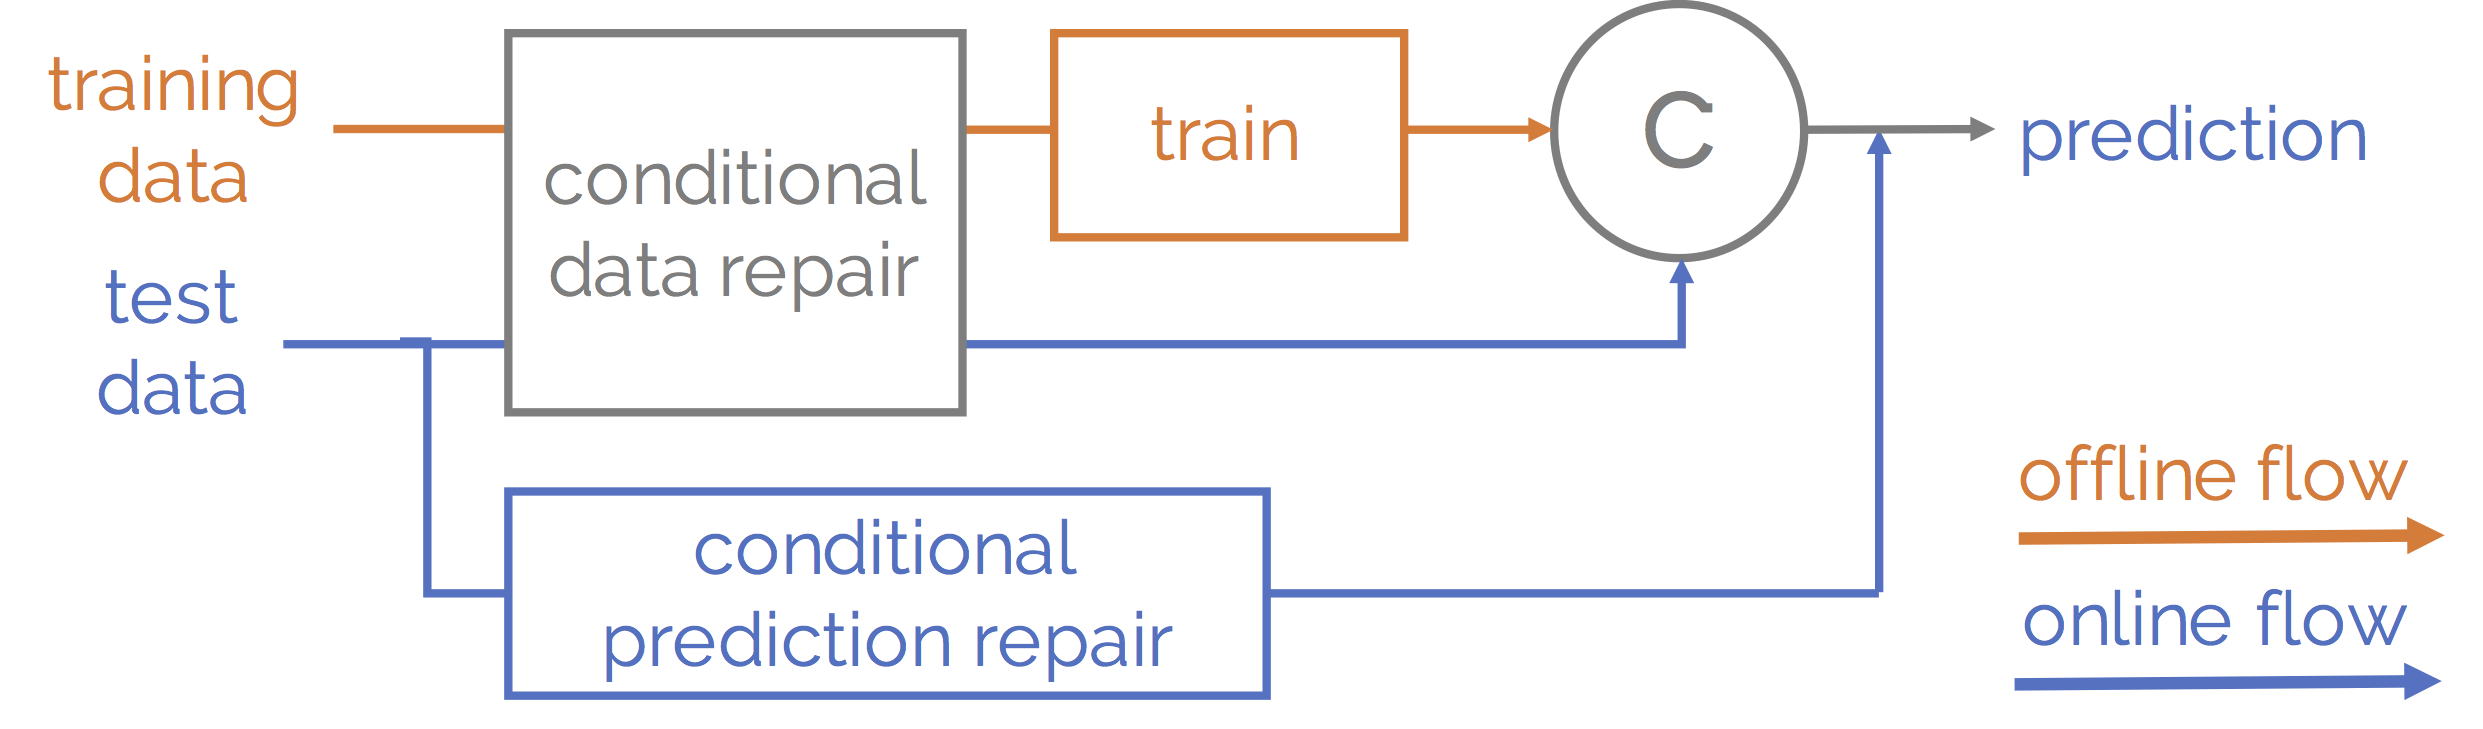
\includegraphics[width=\columnwidth]{figures/workflow.png}
\caption{Offline (\orange{orange}) and online (\blue{blue}) workflows.}
\label{fig:workflow}
\end{figure}

Figure~\ref{fig:workflow} summarizes the training and prediction workflows given the optimal sequence of conditional repairs $\mathcal{L}^*$.  The \orange{orange line} depicts the training process, which first applies the conditional data repairs to the training dataset, and calls \texttt{train()} to generate classifier $C$.  The \blue{blue lines} depict how \sys generates a prediction for a test record: the classifier $C$ makes a prediction using the record cleaned by the conditional data repairs.  In addition, the conditional prediction repair checks the uncleaned test record to decide whether to return the classifier prediction or a default value.


\iffalse
\vspace{0.25em}
\noindent \textbf{Composition Rules: } \sys studies composing data cleaning operations to maximize predictive model accuracy trained on the cleaned data. Now, we need to formalize what it means to compose two data cleaning operations $l_1$ and $l_2$. Recall, that each data cleaning operation is a two-tuple of a predicate and cleaning action $(p, a)$. We define the composition of two operations $l_1=(p_1, a_1)$ and $l_2=(p_2, a_2)$ as generating two new operations (intersection of the predicates, and applying each respective action):
\ewu{is this correct?  should it be $p_1 \wedge p_2$, $p_i \wedge not p_2$
\[
l_1 \circ l_2 := \{(p_1 \wedge p_2, a_1), (p_1 \wedge p_2, a_2)\}
\]
Based on this definition, we can define a restricted library $\mathcal{L}_{\mid l_i}$ that is generated by $l_i$ composed with each of the members of the library:
\[\mathcal{L}_{\mid l_i} = \bigcup_{\forall j \ne i \in \mathcal{L}} l_i \circ l_j \]


\subsection{Extent of Supported Cleaning}
Simply put, \sys cannot support any data cleaning operation that changes the cardinality or labeling of the test dataset.
\reminder{TODO}.
\fi



% We provide an API for users to easily specify derived rules.

\iffalse
    The most basic type of predicate supported by \sys is a \emph{defined} predicate. 
    For example, we could enforce a rule on the running example dataset that every company has greater than 0 employees:
    \[ n\_emp < 0 \] 
    These rules can get more complex and span multiple attributes. For example, if we knew that there were no oil and natural gas companies in the northwest, we could enforce the following detection rule:
    \[ region == USNW \wedge industry == OIL-NG \]
    
    The error detector takes a set of these predicates $\{p_1,...,p_j\}$ and evaluates each one on the dataset to identify cells that are potentially dirty. There will be $j$ total sets of violations, and we denote each set of violations as $\{V_1,...,V_j\}$.
    
    
    
    In contrast to defined rules, \emph{derived rules} are rules that are learned from data.
    The module takes the loaded training dataset $F_{train}, P_{train}$ and returns a predicates $p$.
    An example of a derived rule is  statistical outlier detection, also called Quantitative Error Detection~\cite{hellerstein2008quantitative}.
    For example, one can scan $n\_emp$ calculate the mean value and standard deviation and derive the following rule:
    \[
    abs(n\_emp - mean) > 5*std
    \]
    We provide an API for users to easily specify derived rules.
\fi

\section{Boost-and-Clean}
The key insight of this paper is that the problem described in Section 3.3 can be addressed with statistical boosting.

\subsection{Overview of Boosting}
Ensemble methods construct predictions from combinations of predictors.
Boosting, a type of ensembling, is based on the observation that finding many ``weak learners'' is often significantly easier than finding a single, highly accurate predictor. 
The boosting algorithm calls this ``weak'' or ``base'' learning algorithm repeatedly feeding it a  weighting over the training examples.
Each time it is called, the base learning algorithm generates a new weak prediction rule, and after many rounds, the boosting algorithm must combine these weak learners into a single prediction rule that, hopefully, will be much more accurate than any one of the weak learners.

We will first introduce the classical AdaBoost algorithm for binary classifiers.
This is without a loss of generality since we can use an all-versus-one technique to handle multi-class classification.
The algorithm takes as input a training set of features and labels $(X,Y)$--assume that the labels are $\{-1, 1\}$.
AdaBoost calls a given weak learner repeatedly in a series of rounds. 
The algorithm re-weights the dataset after each round. Initially, all weights are set equally, but on each round, the weights of incorrectly classified examples are increased so that the learner is forced to focus on the hard examples in the training set.

Formally, the AdaBoost algorithm~\cite{freund1995desicion} proceeds as follows:
\begin{algorithm}
\KwData{(X, Y), $\alpha$}
Initialize $W^{(1)}_i = \frac{1}{N}$\\
\For{$t \in [1, T]$}{
  $C_t$ = Train weak learner on dataset weighed by $W^{t}_i$ 
  $W^{(t+1)}_i \propto W^{(t)}_i e^{-\alpha y_i C_t(x_i)}$: down-weigh correct predictions, up-weigh incorrectly predictions.
}
\Return $C(x) = \text{sign}(\sum_t^T \alpha C_t(x) )$
\caption{AdaBoost Algorithm}
\label{alg:adaboost}
\end{algorithm}

\subsection{Why Boosting?}
Each of the library elements define a weak learner.
Given the dataset $R$, we can apply $l_i(R)$ and then train the base classifier $C$. 
The weak learners are evaluated on the clean test labels, which dictates weighting.
Modeling the selecting process as a statistical boosting allows us to make relatively few assumptions about the classifier and the data cleaning operations. 
Instead of having to reason about composing different data cleaning operations (and how compositions may affect accuracy), we are reasoning about a weighted consensus of classifiers trained with different data cleaning approaches.

Furthermore, there is a subtle relationship between this process and feature selection.
Another approach could be to materialize each $l_i(R)$ as another set of features for the classifier and train across the entire library.
This approach makes an assumption that each $l_i$ is simply a row-by-row transformations and cannot discard data or correct a label.

\subsection{Boost-and-Clean Algorithm}
The boosting algorithm proceeds as follows.
Find the $l_i \in \mathcal{L}$ that generates the classifier with highest test accuracy.
Repeat until $B$ cleaning operations are selected, by selecting the operation that performs best on the current ensembles mispredictions and so on.
The result is a new classifier $C_{clean}$ that is derived from the ensemble.

As before, without loss of generality we present the binary classification case with labels in $\{-1,1\}$.
\begin{enumerate}
    \item \textbf{Given (1): } Given the library $\mathcal{L}$ it generates a set of classifiers $\{C^{(0)}, C^{(1)},...,C^{(k)}\}$ where $C^{(0)}$ is the base classifier and $C^{(1)},...,C^{(k)}$ are derived from the cleaning operations.
    \item \textbf{Given (2): } The evaluation dataset $(F_{test}, P_{test})$ with N tuples.
    \item \textbf{Initialize: } $W^{(1)}_i = \frac{1}{N}$
    \item \textbf{For each } $t \in \{1,...,B\}$ 
    \begin{enumerate}
    \item For each $C$ calculate: \[\phi = \sum_i^N = W^{(t)}_i (C(f_i) == p_i)\]
    Select the classifier $j$ with the highest value of $\phi$, denote this as $C_t$.
    \item $W^{(t+1)}_i \propto W^{(t)}_i e^{-\alpha y_i C_t(x_i)}$, which down-weights correctly predicted points and up-weights incorrectly predicted tuples.
    \end{enumerate}
    \item \textbf{Return: } $C(x) = \text{sign}(\sum_t^B \alpha C_t(x) )$  
\end{enumerate}

The intuition for the algorithm is that it focuses every subsequent cleaning operation on the mis-predictions of the current best ensemble.
The algorithm has a few intuitive properties: (1) it prioritizes cleaning operations that improve performance, (2) if no such operations exist it does no worse than the base classifier, and (3) it is agnostic to the implementation of the classifiers.

The basic runtime of the algorithm is polynomial in both the number of cleaning operations and size of the dataset. In the next subsection, we will describe optimizations.

\begin{proposition}[Time Complexity]
The time complexity of Boost-and-Clean is $\mathbf{O}(k^2 N_{test} + k N_{train})$, where $k$ is the number of data cleaning operations, $N_{test}$ is the number of test tuples, and $N_{train}$ is the number of training tuples.
\end{proposition}

Boosting is well-understood statistically, and we can further bound the error on our clean test set (follows from~\cite{schapire2003boosting}):

\begin{proposition}[Error Bound]
For a budget of $B$ cleaning operations, the error rate of Boost-and-Clean on the test dataset decreases as $\mathbf{O}(e^{-2B})$.
\end{proposition}


\subsection{Optimizations and Parallelism}
There are few optimizations that we can apply to make this 
boosting algorithm performant. For these optimizations, we assume that the test dataset fits in memory on a single-node.

\vspace{0.25em}\noindent\textbf{Up-front Materialization: } The first observation is that between iterations the cleaning operations actions do not change--only the way that we score the accuracy. So before running step 4 of the algorithm, we can materialize each of the classifiers predictions on the entire test dataset.
This means for each $f \in F_{test}$, calculate $C_i(f)$ up-front and store it in memory.

\vspace{0.25em}\noindent\textbf{Indexing: } Since we focus on classification, scoring each classifier can be made very efficient with an inverted index.
For each $j$ in the output domain of the classifier $C$, we store an index $j \mapsto \{f : C_i(f) == j\}$.
This allows us to efficiently query the set of points in each round that are mispredicted and correctly predicted.

\vspace{0.25em}\noindent\textbf{Parallelism: }
In Step 4a the algorithm iterates through the list of classifiers, scores each one on the weighted test dataset, and takes the maximum.
This step is embarrassingly parallel and we run each scoring iteration in a separate thread.






\section{The Data Cleaning Library}
 In this section, we describe the architecture and API of the data cleaning library. 
 
\begin{figure}[h]
\centering
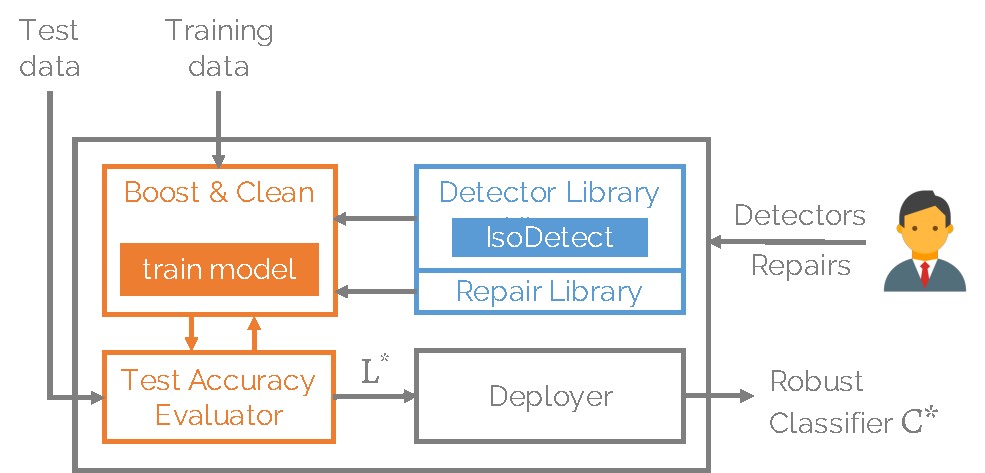
\includegraphics[width=0.8\columnwidth]{figures/arch.pdf}
\caption{\sys system architecture.}
\label{f:arch}
\end{figure}

\subsection{Architecture}
The architecture of \sys includes three high-level components: (1) a loader, (2) error detector, and (3) repair action selector.
The loader takes in a weakly structured dataset (e.g., a CSV file) parses the file and returns a relation over a set of attributes and associated data types with each attribute.
Then, this relation is passed into an error detector.
The error detector identifies a candidate set of erroneous records and taxonomizes them into group of violated constraints.
Finally, associated with each of the violated constraint are repair actions (described in Section 3).
This modular architecture allows us to build a large number of library components, where users can specify additional rules for error detection without having to specify repair actions.
This section will overview the architecture of each of the components (including error detection) and the next section will go into the implementation details of the error detection module.

\subsection{Error Detection}
We noticed that many derived rules follow a similar structure.
First, they convert a row into a feature vector (in the above example, trivially projecting onto $num\_employees$).
Next, they apply a threshold (possibly multi-dimensional) on the feature vector.
We propose a modular architecture that has a single outlier detection technique (called Isolation Forests) at the end of the pipeline but allows for different types of featurization.
User defines a function that maps a row to a vector in $\mathbb{R}^d$ and the Isolation Forest identifies outliers in this space.
For a scalar feature in $\mathbb{R}$, the Isolation Forest degenerates into a threshold rule. 
We experimented with alternative outlier detection techniques (e.g., Minimum Covariance Determinant) but found that the Isolation Forest provided the best tradeoff between runtime and accuracy.

While the availability of such rules is a typical assumption in data cleaning~\cite{DBLP:conf/sigmod/ChuIKW16},  defining such rules requires extensive domain knowledge and is time-consuming.
One of our design objectives is to minimize the burden on data scientists, so we provide an initial library of rules which are described in the next section.
These rules are not meant to replace domain knowledge but rather to address routine problems seen across many different datasets.



\subsection{Loader}
The first step in using \sys is loading a dataset. \sys requires that that data is initially weakly structured, similar to the assumptions of SQLShare~\cite{howe2013sqlshare}. It assumes that each row corresponds to a record and attributes are delimited, but there are potentially missing values, the domain of possible attribute values are unknown, and the data types are unknown.
We implemented a schema-on-read loading module that takes as input a SQL table, CSV, or a text file.
This module returns a structured relation of tuples and inferred data types for each attribute (numerical, categorical, string, date, address).
We designed the type inference to be soft--allowing for errors to exist in the dataset.
The module automatically builds indices over the numerical and categorical attributes.
These indices will help optimize the error detection module.



\subsection{Cleaner}
Given a set of detected violations $\{V_1,...,V_j\}$, the cleaner assigns a tuple possible repair action to each $V_i$ (one if the data is in training, one if the data is in test).
Repairs are applied as a batch to each set of violations and not in a per-cell basis.
The available options are:
\begin{enumerate}
    \item \emph{Impute the mean (Train and Test): } Impute a cell in violation with the mean value of the attribute calculated over the training data excluding violated cells.
    \item \emph{Impute the mode (Train and Test): } Impute a cell in violation with the most frequent value of the attribute calculated over the training data excluding violated cells.
    \item \emph{Impute the median (Train and Test): }Impute a cell in violation with the median value of the attribute calculated over the training data excluding violated cells.
     \item \emph{Discard (Train Only): } Discard a row with a violated cell from the training dataset.
     \item \emph{Fail-Safe (Test Only): } Automatically predict the most-frequent label for a row with a violated cell.
\end{enumerate}

The cleaner's role is to learn an assignment of these actions to each of the violations.
The combination of the actions and the predicates define the data cleaning libary $\mathcal{L}$.








%\section{Pre-populated Detectors}
We initialized the error detection module with defined and derived rules that are domain-agnostic.
We anticipate that users will build on these rules for specific use-cases.

\subsection{Observations from Real Data}
Abedjan et al. provide an extensive experimental evaluation of error detection techniques on real datasets~\cite{DBLP:journals/pvldb/AbedjanCDFIOPST16}.
The results of Abedjan et al. suggests that the datasets contain an interesting structure that can be exploited to pre-populate the library.
3 out of the 5 experimental datasets contained significant amounts of missing value constraints--which can largely be detected with sensible heuristics (e.g., hard-coded checks for NULL entries, No Alpha Numeric Characters, N/A, None).
On one of the remaining datasets, a Functional Dependency violation was correlated with erroneous numerical attribute values allowing it to be detected with quantitative methods.
And only the final dataset required a complex user-specified Denial Constraint to detect errors. 

In summary on 4 out of 5 datasets, a significant portion of errors, were essentially \emph{domain integrity} errors, i.e., a cell with a value not contained in the set of permissible values.
We argue that with appropriate featurization such constraints can be learned from data or can be identified by heuristics--and for the remaining errors user-specified constraints are necessary.
On 8 experimental datasets, our detector achieves a detection accuracy of 81\% of all of the errors found by hand-written rules.

\subsection{Heuristics}
In a first pass, we apply a collection of heuristics to detect obvious inconsistencies and type signature violations. These heuristics are implemented as \emph{defined} rules in the architecture.

\vspace{0.5em}
\noindent\textbf{Missing Values: }  We enumerate a set of patterns which commonly describe missing values in a database. This includes attributes that are actually \textsf{NULL}, empty strings, NaN, Inf, or otherwise lack alphanumeric characters.

\vspace{0.5em}
\noindent\textbf{Parsing/Type Errors: } Since each attribute is tagged with a type signature, we can evaluate if a value matches the type. For numerical values, this means that the entry can be parsed into a floating point number or an integer. For dates and addresses this means that the entry has a minimum of the required components (Month, Day, Year) or (Street, City, State).

\subsection{Detecting Quantitative Errors}
In addition to the heuristics, we project the dataset to retain just the numerical attributes and apply quantitative outlier detection techniques.
This module is implemented as a \emph{derived} rule in the architecture.
In numerical outlier detection the goal is to estimate the \emph{true} spread of a distribution and use that to threshold values that lie outside the spread.
The key challenge in outlier detection is that the outliers can affect one's estimate of a distribution's spread.

One approach is the Minimum Covariance Determinant (MCD), which is a robust estimator of the variance of a set of numbers, and has been used in a several recent works on numerical outlier detection (most notably MacroBase~\cite{bailis2016macrobase}).
We experimentally found that this approach is computation expensive and has a number of subtleties in implementation (like handling rank-deficient covariance matrices).
Instead, we found that a variant of Random Forest classification, called an Isolation Forest, was better suited for the problem.
The Isolation Forest isolates observations by randomly selecting a feature and then randomly selecting a split value between the maximum and minimum values of the selected feature.
Since recursive partitioning can be represented by a tree structure, the number of splittings required to isolate a sample is equivalent to the path length from the root node to the terminating node.
This path length, averaged over a forest of such random trees, is a measure of abnormality and our decision function.
Since these splits are axis aligned they can be efficiently compiled into threshold rules that can be evaluated on future data.

\subsection{Other Errors: Word2Vec Featurization}
However, quantitative errors are not a panacea and the difficulty in data quality research has been detecting errors that span multiple heterogenous attributes.
In principle, statistical outlier detection techniques can apply to featurized data.
The challenge is that naive featurization can explode the dimensionality of the feature space. Even a two-attribute relation with one numerical and one string-valued attribute, may have 1000s of features if one chooses a bag-of-words representation for the string-valued attribute.
The statistical power of outlier detection techniques rapidly diminish in the high-dimensional feature-spaces and the discrete distribution of feature vectors (e.g., bag-of-words) may violate the smoothness assumptions needed by the approaches.

One approach is to borrow recent results from Natural Language Processing using Neural Networks to first embed the records in a vector-space and then apply outlier detection techniques. The \textsf{word2vec} model \cite{mikolov2013distributed} is one such approach.
Using large amounts of unannotated plain text, \textsf{word2vec} learns relationships between words automatically with a Neural Network that predicts the occurrence of nearby words.
 Each word is assigned a vector in the vector space such that words that share common contexts (i.e., occur in the same document) in the corpus are located in close proximity to one another in the space.
 This vector space captures semantic relationships between words.
 
 We can adapt \textsf{word2vec} for featurizing records in a relation. Each record is treated as a document and each attribute is treated as word.
 The model is then trained using all of the records in the training dataset.
 Thus, for each attribute value we have a vector.
 To featurize a record, we concatenate these vectors together.
 Therefore, for each record $r$ there is an associated vector $r_v$.
  Like the NLP application, this vector space captures semantic relationships between records.
  We empirically find that applying the Isolation Forest outlier detection in this space leads to improved results.
We noticed that the quantitative outlier detection and word2vec both used the Isolation Forest as the main primitive, but with different featurizations.






%\section{The Data Cleaning Library}
 In this section, we describe the architecture and API of the data cleaning library. 
 
\begin{figure}[h]
\centering
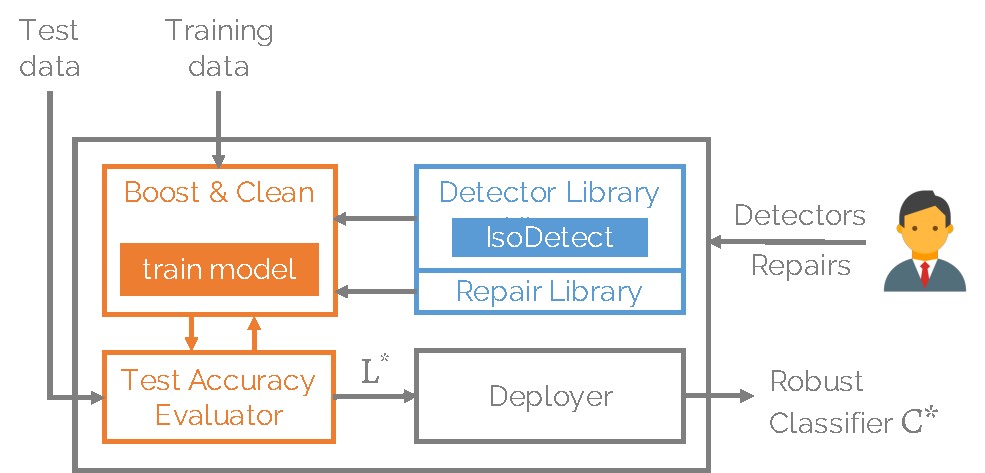
\includegraphics[width=0.8\columnwidth]{figures/arch.pdf}
\caption{\sys system architecture.}
\label{f:arch}
\end{figure}

\subsection{Architecture}
The architecture of \sys includes three high-level components: (1) a loader, (2) error detector, and (3) repair action selector.
The loader takes in a weakly structured dataset (e.g., a CSV file) parses the file and returns a relation over a set of attributes and associated data types with each attribute.
Then, this relation is passed into an error detector.
The error detector identifies a candidate set of erroneous records and taxonomizes them into group of violated constraints.
Finally, associated with each of the violated constraint are repair actions (described in Section 3).
This modular architecture allows us to build a large number of library components, where users can specify additional rules for error detection without having to specify repair actions.
This section will overview the architecture of each of the components (including error detection) and the next section will go into the implementation details of the error detection module.

\subsection{Error Detection}
We noticed that many derived rules follow a similar structure.
First, they convert a row into a feature vector (in the above example, trivially projecting onto $num\_employees$).
Next, they apply a threshold (possibly multi-dimensional) on the feature vector.
We propose a modular architecture that has a single outlier detection technique (called Isolation Forests) at the end of the pipeline but allows for different types of featurization.
User defines a function that maps a row to a vector in $\mathbb{R}^d$ and the Isolation Forest identifies outliers in this space.
For a scalar feature in $\mathbb{R}$, the Isolation Forest degenerates into a threshold rule. 
We experimented with alternative outlier detection techniques (e.g., Minimum Covariance Determinant) but found that the Isolation Forest provided the best tradeoff between runtime and accuracy.

While the availability of such rules is a typical assumption in data cleaning~\cite{DBLP:conf/sigmod/ChuIKW16},  defining such rules requires extensive domain knowledge and is time-consuming.
One of our design objectives is to minimize the burden on data scientists, so we provide an initial library of rules which are described in the next section.
These rules are not meant to replace domain knowledge but rather to address routine problems seen across many different datasets.



\subsection{Loader}
The first step in using \sys is loading a dataset. \sys requires that that data is initially weakly structured, similar to the assumptions of SQLShare~\cite{howe2013sqlshare}. It assumes that each row corresponds to a record and attributes are delimited, but there are potentially missing values, the domain of possible attribute values are unknown, and the data types are unknown.
We implemented a schema-on-read loading module that takes as input a SQL table, CSV, or a text file.
This module returns a structured relation of tuples and inferred data types for each attribute (numerical, categorical, string, date, address).
We designed the type inference to be soft--allowing for errors to exist in the dataset.
The module automatically builds indices over the numerical and categorical attributes.
These indices will help optimize the error detection module.



\subsection{Cleaner}
Given a set of detected violations $\{V_1,...,V_j\}$, the cleaner assigns a tuple possible repair action to each $V_i$ (one if the data is in training, one if the data is in test).
Repairs are applied as a batch to each set of violations and not in a per-cell basis.
The available options are:
\begin{enumerate}
    \item \emph{Impute the mean (Train and Test): } Impute a cell in violation with the mean value of the attribute calculated over the training data excluding violated cells.
    \item \emph{Impute the mode (Train and Test): } Impute a cell in violation with the most frequent value of the attribute calculated over the training data excluding violated cells.
    \item \emph{Impute the median (Train and Test): }Impute a cell in violation with the median value of the attribute calculated over the training data excluding violated cells.
     \item \emph{Discard (Train Only): } Discard a row with a violated cell from the training dataset.
     \item \emph{Fail-Safe (Test Only): } Automatically predict the most-frequent label for a row with a violated cell.
\end{enumerate}

The cleaner's role is to learn an assignment of these actions to each of the violations.
The combination of the actions and the predicates define the data cleaning libary $\mathcal{L}$.









%\section{Cleaner}
After the detector returns $C_{d}$, the cleaner applies one of three actions: (1) impute the cell with a sensible default (consistent null symbol, mean value, most frequent value), (2) remove the record from the training set, or (3) flag the record as ``unpredictable'' return a null prediction or the most frequent label. The challenge is that search space is exponential in the number of cells. To address this problem, we use the prediction accuracy oracle to prioritize errors that correlate strongly with model mispredictions. This often greatly reduces the search space to a handful of sub-populations of data. \reminder{Sk needs to implement. We apply x algorithm to efficiently decide a per-cell repair}. For each cell $c \in C_{d}$, the cleaner returns a corresponding edit $e$.
%\section{Synthesizer}
Given a the list of edits and cells, the synthesizer generates a Python program that given future unlabeled dirty data in the same schema will predict the the label. \sys converts the proposed edits into a lambda without any import dependencies. This allows for the detection predicate to be efficiently evaluated on new data, as well as be serialized so it can on future data without having to be retrained.

\section{Experiments}\label{s:exp}
In this section, we present the results of our experiments.  We execute \sys on $13$ datasets based on three sets of real-world cases---machine learning competitions, data analysis pipelines, and \company---and report accuracy measures and end-to-end runtime.  Then, we present a series of micro-benchmarks that evaluate each of the modules of \sys.  Our goal is to understand the conditions where automated cleaning is able to accurately detect and repair data in a way that improves the held-out test accuracy.

\subsection{Baselines and Methods}
To the best of our knowledge, there does not exist a comparable general purpose ML+Data Cleaning system to \sys in industry or academia.
We evaluate \sys against a number of baseline approaches inspired by solutions proposed in literature. 

\vspace{0.25em}\noindent\textbf{No Cleaning (NC): } We train a model without any modification to the training or test data.

\vspace{0.25em}\noindent\textbf{Quantitative (Q): } We train a model where only quantitative outliers in both training and test are imputed with a mean value. \ewu{Are outliers detected using isolation forest + numerical attribute featurizer?} 

\vspace{0.25em}\noindent\textbf{Integrity Constraint (IC): } We read through each dataset to identify a set of anomalous values for each attribute on a best-effort basis.  We then codified these as integrity constraint rules, and corrected the identified errors using a statistical distortion minimization metric as in~\cite{prokoshyna2015combining}.\ewu{  In one sentence what is the statistical distortion min metric}

\vspace{0.25em}\noindent\textbf{Quantitative + IC (Q+IC): } We use the quantitative and integrity constraints for detection; we use mean and mode imputation as repair functions for numerical and text attributes, respectively.

\vspace{0.25em}\noindent\textbf{Best Single (Best-1): } We run \sys with $B=1$ and identify the  single best conditional repair.

\vspace{0.25em}\noindent\textbf{Worst Single (Worst-1): } We run \sys with $B=1$ and identify the single worst conditional repair..

\stitle{BC-3: } We run \sys with $B=3$.

\stitle{BC-5: } We run \sys with $B=5$.


\vspace{0.25em}

\ewu{NEED TO EXPLAIN WHAT TEST DATASET IS.}


In all of our experiments, we used standard classification models and featurization techniques from Python \textsf{sklearn}.
The classifiers were trained in Python 2.7 and timing experiments were run on an Amazon EC2 m4.16xlarge instance\footnote{64 virtual cpus and 256 GiB memory}.
To avoid overfitting, we carefully designed the accuracy evaluation experiments for \sys by using a ``doubly'' held out test dataset: the test dataset used to optimize \sys is different from a completely unseen test dataset that is solely used to report the final prediction accuracy.
We describe hyper-parameter settings for each technique in the text of each experiment.

We used the \textsf{sklearn} Random Forest classifier with custom depth and branch parameters.  The training procedure uses a set of standard featurizers (hot-one encoding for categorical data, bag-of-words for string data, numerical data as is) in a similar fashion as~\cite{DBLP:conf/sigmod/GokhaleDDNRSZ14}.  Note that these featurizers are used as part of the black-box training procedure and are distinct from those used in the detector generator library.




\begin{table*}[t]
\centering
\label{tab:accuracy}
\begin{tabular}{|l|r|r|r|r|r|r|r|r|r|}
\hline
ML Competition& NC & Q &	IC & Q+IC &	Best-1 &	Worst-1 &	BC-3 & BC5 & Rel. Improvement\\
\hline
USCensus	&0.85&	0.82&	0.86&	0.84&	0.87&	0.79&	0.88&	\blue{0.91} & +4.5\% \\
Emergency &	0.67&	0.72&	0.67&	0.72&	0.72&	0.66&	0.72&	\blue{0.75} & +4.7\%\\
Sensor	&0.92&	0.93&	0.92&	0.89&	0.92&	0.8&	\blue{0.94}&	0.94 & +1.3\%\\
NFL	&0.74&	0.74&	0.76&	0.75&	0.76&	0.74&	0.79&	\blue{0.82}& +5.1\%\\
EEG	&0.79&	0.82&	0.79&	0.83&	0.83&	0.7&	0.85&	\blue{0.89}& +6.8\%\\
Titanic	&0.83&	0.72&	0.83&	0.76&	0.83&	0.69&	0.83&	\blue{0.84}& +1.1\%\\
Housing	&0.73&	0.76&	0.73&	0.77&	0.77&	0.65&	\blue{0.81}&	0.76& +5.1\% \\
Retail	&0.88&	0.88&	0.91&	0.91&	0.91&	0.87&	0.94&	\blue{0.95}& +4.3\% \\
\hline
\hline
Data Analytics & NC & Q &	IC & Q+IC &	Best &	Worst &	BC-3 & BC5 & Rel. Improvement\\
\hline
FEC  & 0.62 & 0.53 & 0.61 & 0.57 & 0.71 & 0.51 & 0.74 & \blue{0.77} &  +8.4\% \\
Restaurant (Multiclass) & 0.42 & 0.42 & 0.58 & 0.68 & \blue{0.62} & 0.36 & 0.61 & 0.60 & (1.61)\% \\
\hline
\hline
Company X & NC & Q &	IC & Q+IC &	Best &	Worst &	BC-3 & BC5 & Rel. Improvement\\
\hline
Dataset 1 (AUC) &0.60& & & &0.61& & &0.66& 0.69\\
Dataset 2 & & & & & & & & &\\
Dataset 3 & & & & & & & & &\\
\hline
\end{tabular}
\caption{End-to-end accuracy results for each dataset and experimental method. We report standard classification accuracy.  The right column summarizes the accuracy improvement relative to the best non BC-3/5 approach.}
\end{table*}


\subsection{End-to-End Accuracy}
In our first experiment, we evaluated the accuracy of \sys compared to the baselines.
We tried to minimize hyper-parameter tuning as much as possible to simulate a real-scenario where extensive tuning and parameter search might be expensive.


\subsubsection{ML Competition Datasets}\label{exp:comp}
We downloaded 8 binary classification datasets from Kaggle competitions and benchmarks in the UCI ML repository.  \ewu{The next two sentences seem contradictory: they are clean, but dirty} These datasets are mostly clean as they have been extracted, structured, and published.
Nevertheless, they contain missing values, numerical outliers, and pattern errors (oddly formatted values).
For this set of experiments, we used a single hyper-parameter setting for all the detectors and classification models (default \textsf{sklearn} library setting). \ewu{IMPORTANT: SOMEWHERE IN THE WRITING, WE FORGOT TO TALK ABOUT HYPERPARAMETERS}

We briefly describe each dataset and their errors below:

\vspace{0.5em}\noindent\textbf{USCensus: } This dataset contains US Census records for adults and the goal is to predict  whether the adult earns more than $50,000$ dollars. It contains 32,561 records with 15 numerical and categorical attributes. Examples of data error include:
\begin{lstlisting}
#missing values
40,Private,121772,Assoc-voc,11,
Married-civ-spouse,Craft-repair,Husband, 
Asian-Pac-Islander,Male,0,0,40,(*\orange{\bf{?}}*),>50K

#coding inconsistency
57,Local-gov,110417,HS-grad,9,
Married-civ-spouse,Craft-repair,Husband,
White,Male,(*\orange{\bf{99999}}*),0,40,United-States,>50K
\end{lstlisting}

\vspace{0.5em}\noindent\textbf{NFL: } This dataset contains play-by-play logs from US Football games. The dataset contains 46,129 records with 65 numerical, categorical, and string-valued attributes. Given the record, the classification objective is to determine whether the next play the team runs is a run or a pass play.
The dataset contains a significant number of missing values and ``sentinel'' records that mark the end of a log sequence:\ewu{What distinguishes a sentinel?}
\begin{lstlisting}
#missing values
"36",2015-09-10,"2015091000",1,1,(*\orange{\bf{NA}}*),"15:00",
15,3600,0,"NE",35,35,0,0,0,(*\orange{\bf{NA}}*),"PIT","NE"(*\blue{\bf{....}}*)

#sentinel record
"189710",2016-01-03,"2016010310",10,2,NA,"00:00",
0,1800,8,"GB",17,17,0,-1,0,0,"",NA,"END(*~*)QUARTER2"
,1,0,0,0,NA, NA,NA,0,"Quarter(*~*)End"(*\blue{\bf{....}}*)
\end{lstlisting}

\vspace{0.5em}\noindent\textbf{EEG: } This dataset contains \ewu{SANJAY DESCRIBE}
\begin{lstlisting}

\end{lstlisting}

\vspace{0.5em}\noindent\textbf{Emergency: } This dataset contains records on 911 calls from Pennsylvania. There are 111,766 records with 9 attributes. Given the record, the classification challenge is to determine whether the emergency service response time will be less than $5 min$. This dataset contains missing values, and spurious locations not served by the 911 center:
\begin{lstlisting}
#missing values
41.1671565,-76.8740304,MAIN;(*\orange{\bf{--}}*); Station 308A;
2016-01-02 @ 13:01:30;,17752,EMS: UNKNOWN MEDICAL
EMERGENCY,2016-01-02 13:06:00,(*\orange{\bf{--}}*),MAIN,1

#spurious location (outisde 100 mile radius)
(*\orange{\bf{41.1671565,-76.8740304,}}*)MAIN;(*\orange{\bf{--}}*); Station 308A;
2016-01-02 @ 13:01:30;,17752,EMS: UNKNOWN MEDICAL 
EMERGENCY,2016-01-02 13:06:00,(*\orange{\bf{--}}*),MAIN,1
\end{lstlisting}

\vspace{0.5em}\noindent\textbf{Sensor: } The Intel sensor dataset~\cite{} contains 928,991 temperature, humidity, and light sensor readings a sensor deployment. The classification task is to predict whether the readings came from a particular sensor (sensor 49). This dataset has numerical outliers:
\begin{lstlisting}
#Normal Record
49  -0.999750  12.862100  10.368300  10.438300  
11.669900 (*\orange{\bf{13.493100}}*)  13.342300  8.041690  
8.739010  26.225700  59.052800

#Spurious Record
49  1.175188  12.279100  8.849360  9.005830  
10.111700  (*\orange{\bf{378.750000}}*)  19.319400  15.916200  
37.631400  27.150100  53.403700
\end{lstlisting}

\vspace{0.5em}\noindent\textbf{Titanic: } This dataset contains 891 records from the Titanic manifest with 12 attributes. The classification objective is to determine whether the passenger survived or not. There are missing values and string formatting errors:

\begin{lstlisting}
#missing values
891,0,3,"Dooley, Mr. Patrick",male,
32,0,0,370376,7.75,(*\orange{\bf{--}}*),Q
\end{lstlisting}

\vspace{0.5em}\noindent\textbf{Housing: } The housing dataset contains 1460 records and 81 attributes of house price listings. The classification objective is to determine whether the listed house will be sold above 750000. 
This dataset contains missing values as well as numerical outliers:
\begin{lstlisting}
#missing values
(*\blue{\bf{....}}*)204,228,0,0,0,(*\orange{\bf{NA,NA}}*),Shed,350,11,2009,WD,
Normal,200000
\end{lstlisting}

\vspace{0.5em}\noindent\textbf{Retail: } The online retail dataset contains 541,909 records of online retail purchases with 8 attributes. The classification objective is to predict whether the purchase occurred in the United Kingdom.
This dataset contains numerical errors where some purchased quantities are reported as negative:
\begin{lstlisting}
#outliers
C536391,21980,PACK OF 12 RED RETROSPOT TISSUES
,(*\orange{\bf{-24}}*),12/1/10 10:24,0.29,17548,United Kingdom
\end{lstlisting}

\vspace{1em}
The first set of rows in Table \ref{tab:accuracy} present the predictive accuracy of models trained with \sys on the completely unseen test data.  In all experiments, the model trained with one of the \sys  approaches was the most accurate.
The quantitative baseline performed well when the errors were clear numerical outliers (e.g., Sensor and  EEG).  However, its performance suffered in datasets with missing values or formatting errors, and {\it degraded model accuracy} in the US Census dataset.
Conversely, the integrity constraint approach worked well for non-numerical errors, however it was not useful for Emergency, EEG, Housing, nor Sensor.
The naive union of (Q+IC) has difficulty composing the two operations in the US Census dataset and degrades accuracy as compared to quantitative or integrity constraint alone in several datasets.  Finally we compare and find up to a 14\% difference between the best and worst repairs when using \sys.  These results emphasize the need for an automatic search solution that can avoid repairs that are ineffective or reduce accuracy.

\ewu{What about BC3 and BC5}


\subsubsection{Data Analytics}
The next class of datasets that we considered were datasets known to have significant errors--unlike the relatively clean competition datasets. These are two datasets that were used in previous data cleaning papers, and we designed classification tasks based on the datasets.
Unlike the ML competition datasets, we tuned the classifier and detector hyperparamters for each dataset. 
The accuracy results are presented in the second set of rows in Table \ref{tab:accuracy}.

\vspace{0.5em}\noindent\textbf{Federal Election Commission Contributions: } The FEC provides a dataset of election contributions of 6,410,678 records with 18 numerical, categorical and string valued attributes. This dataset has a number of errors. There are missing values, formatting issues (where records have the wrong number of fields causing misaligment in parsing), and numerical outliers (negative contributions).

\begin{lstlisting}
#missing values
C00458844,"P60006723","Rubio, Marco","RUCINSKI,
ROBERT","APO","AE","090960009","US ARMY",
"PHYSICIAN",100,08-MAR-16,(*\orange{\bf{``''}}*),(*\orange{\bf{``''}}*),(*\orange{\bf{``''}}*),"SA17A",
"1082559","SA17.1074981","P2016"

#misalignment
C00458844, "P60006723", (*\orange{\bf{"Rubio", "Marco"}}*), "BRIZOLIS",
" DEMETRI MR.", "RANCHO SANTA FE", "CA", 
"920674357", "RETIRED", "RETIRED", 100, 
28-OCT-15, "", "", "", "SA17A", "1047126", 
"SA17.851920", "P2016"

#rejected contributions double recorded
C00458844,"P60006723","Rubio, Marco","SWAID, 
SWAID N. DR.","BIRMINGHAM","AL","352660827",
"NEWOLOGICAL SURGERY ASSOCIATES","PHYSICIAN",
(*\orange{\bf{-400}}*),28-DEC-15, "REDESIGNATION TO GENERAL","X",
"REDESIGNATION TO GENERAL","SA17A",
"1047126","SA17.892835B","P2016"

C00458844,"P60006723","Rubio, Marco","SWAID, 
SWAID N. DR.","BIRMINGHAM","AL","352660827",
"NEWOLOGICAL SURGERY ASSOCIATES","PHYSICIAN",
(*\orange{\bf{400}}*),28-DEC-15, 
"REDESIGNATION FROM PRIMARY","X", 
"REDESIGNATION FROM PRIMARY","SA17A",
"1047126","SA17.918421","G2016"
\end{lstlisting}

Our classification objective was to determine whether the contribution would be above or below $100$ dollars. Due to the severity of the errors in the dataset, there is nearly a 15\% difference between the prediction accuracy of a classifier with and without \sys.
Furthermore, a purely quantitative approach is not useful for this dataset.
An integrity constraint based method improves accuracy but the automatic imputations are unreliable on this data.
Furthermore, it is difficult to express a problem like row misalignment as a integrity constraint.

We find empirically that the alignment is better detected by the word2vec error detector in \sys.
As a result the best single cleaner is using the word2vec error detector.
This is improved by combining this with quantitative checks for numerical outliers and missing values.
In all, \sys with a budget of 5 improves accuracy 8.4\% over the best single cleaner. 

\vspace{0.5em}\noindent\textbf{Restaurant Dataset: } The restaurant dataset has 758 distinct records and 4 attributes. This dataset has typically been used as a benchmark for entity resolution since records are duplicated with minor inconsistencies.
We designed a multi-class classification task to see if we could predict the city from record.
One of the major inconsistencies was additional attributes appended to the restaurant category.

\begin{lstlisting}
campanile,624 s. la brea ave.,los angeles,
american

grill  the,9560 dayton way,beverly hills,
american (*\orange{\bf{(traditional)}}*)
\end{lstlisting}

On this dataset, we see a negative result from \sys. Our test error decreases as we increase the number of selected cleaners. We speculate this is due to overfitting due to the extremely small size of the dataset  ($<1000 records$) combined with the expressiveness of the classifiers model.

\subsubsection{Company X Experiments}
We applied \sys to three datasets from Company X.

\reminder{TODO Write Description}

\begin{figure}[t]
\centering
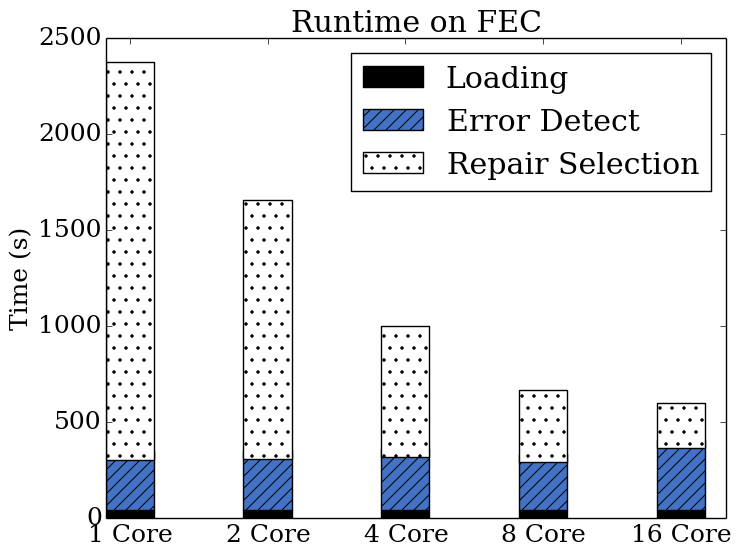
\includegraphics[width=0.8\columnwidth]{exp/runtime.png}
\caption{(A) This plot measures the run-time on a 6M record dataset (1.5GB) grouped by the number of cores on the machine. The repair selection scales but the other steps are not parallelized.\label{exp:runtime}}
\end{figure}

\begin{figure}[t]
\centering
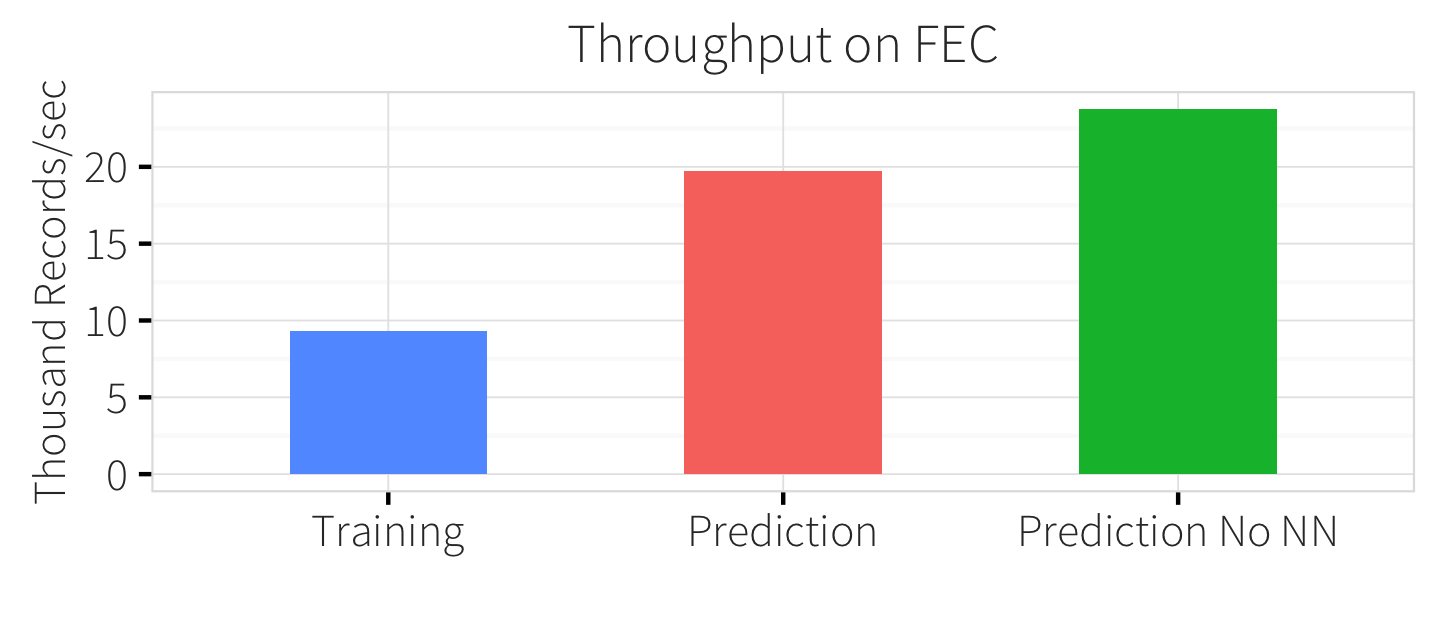
\includegraphics[width=0.8\columnwidth]{exp/runtime2.png}
\caption{We plot the prediction and training throughput for 16-cores. Prediction throughput is much higher than training throughput.\label{exp:tp}}
\end{figure}

\subsection{End-to-End Run Time}
Next, we evaluate the end-to-end wall clock runtime of \sys. We use the FEC dataset since it is the largest. This evaluation includes all of the optimizations for \sys. The FEC dataset is 1.5 GB (about 6M records). 
Figure \ref{exp:runtime} plots the results.
With a single core, \sys takes 2422 seconds in wall-clock time. Of that time, 2072 seconds is spent in repair selection, 306 seconds is spent in error detection, and 44 seconds in loading the dataset.
We can parallelize the repair selection step. We parallelize the inner-loop of the boosting algorithm. On 16-cores, we are able to reduce the runtime of the repair selection to 212 seconds. This constitutes a 9.7x speedup for that step.

It is important to note that this latency is only incurred during training. During prediction, the learned model can be applied, and this process is much faster than training. 
Figure \ref{exp:tp} plots the throughput of \sys.
The number of records that can be processed per second on 16 cores for prediction is 19746 records/second, but during training it is 9316 records/second. One of the key bottlenecks is evaluating the word2vec model for each prediction, and without this model, the throughput increases to 23746 records/second.

\begin{figure}[t]
\centering
 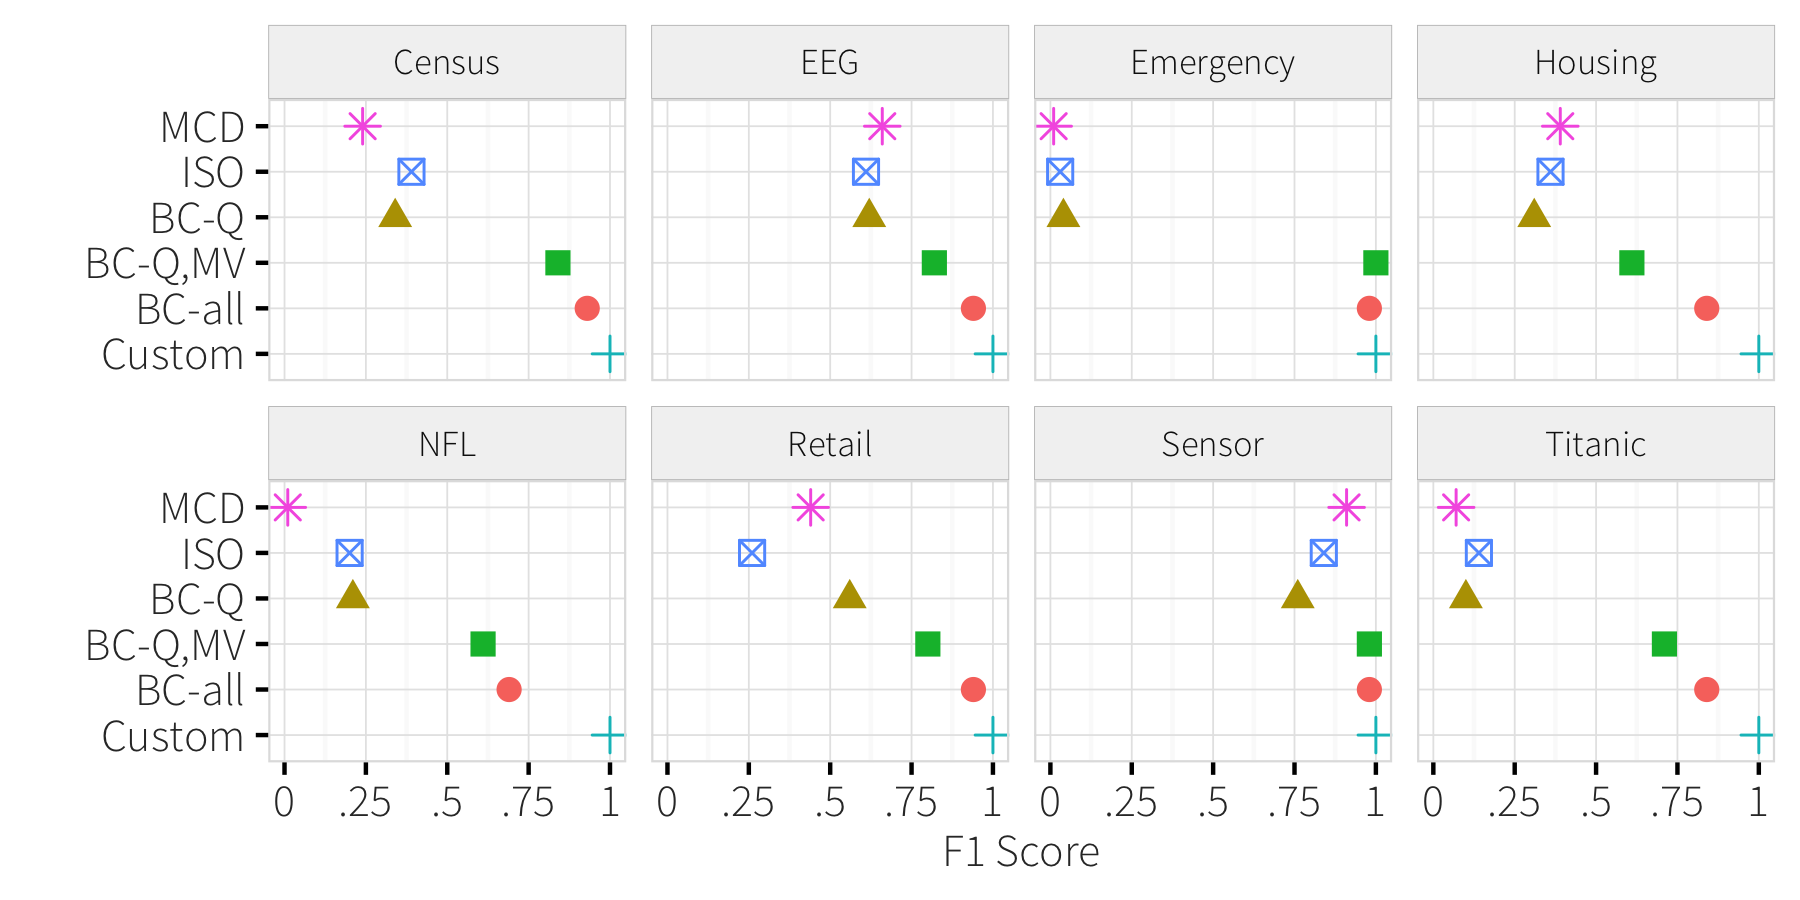
\includegraphics[width=\columnwidth]{exp/daccuracy.png}
 \caption{On 8 Machine Learning competition datasets, we evaluated the F1 accuracy score of different error detection techniques. We compare against Isolation Forest (alone), Minimum Covariance Determinants, and Hand-Written rules. We evaluate \sys using only the Isolation forest for numerical outliers, outliers+missing values, and outliers+missing values+word2vec.
 The final detector in \sys achieves up to 81\% of the accuracy on the competition datasets.
 \label{fig:derror}}
\end{figure}

\begin{figure}[t]
\centering
 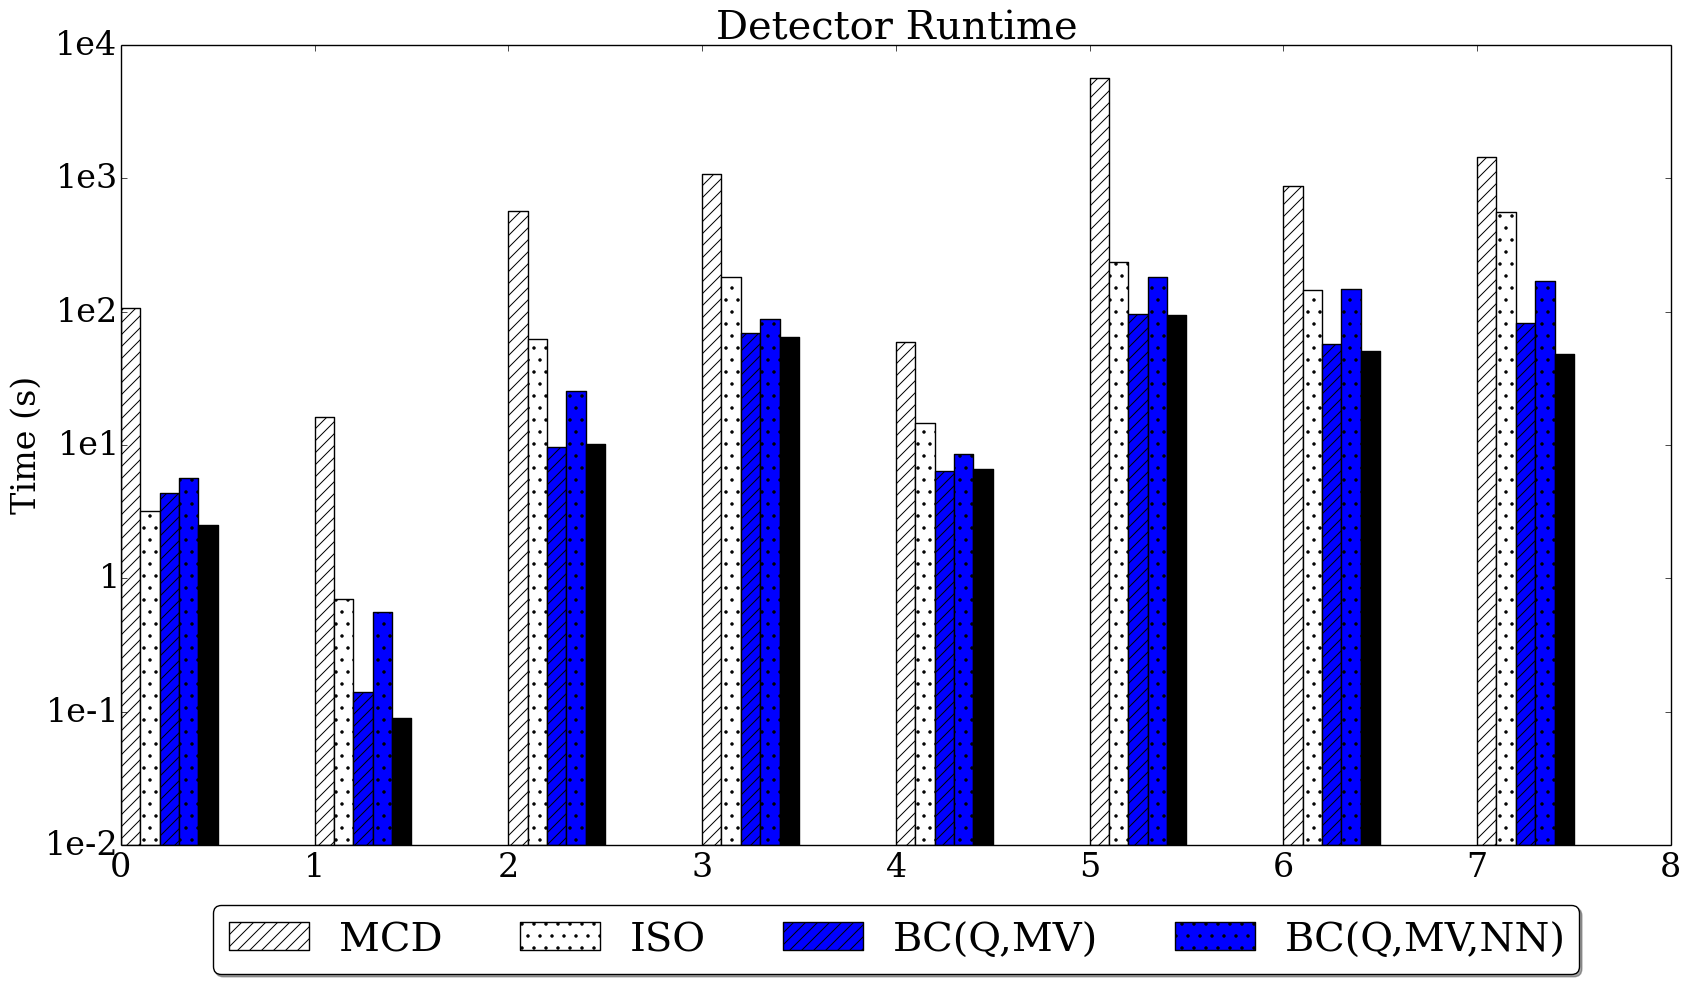
\includegraphics[width=\columnwidth]{exp/druntime.png}
 \caption{On 8 Machine Learning competition datasets, we evaluated the runtime of each of the detection methods. We compare against Isolation Forest, Minimum Covariance Determinants, and Hand-Written rules. While evaluating hand-written rules is certainly faster, \sys is faster in terms of wall-clock time than MCD.
 \label{fig:druntime}}
\end{figure}

\subsection{Micro-Benchmarks}
Next, we evaluate the different components of \sys in terms of accuracy and runtime.

\subsubsection{Detectors}
The first component that we evaluate are the detectors. We design a set of automatic error detectors based on heuristics, statistical criteria, and the word2vec neural network. We first measure its accuracy against hand-written detection scripts, and other quantitative outlier detection techniques (Isolation Forests and Minimum Covariance Determinants).
\sys internally uses an Isolation Forest combined with other error detectors, so we evaluate \sys with and without certain detection modules.
We measure accuracy w.r.t the alternatives with the F1 accuracy measure.

 Figure  \ref{fig:derror} shows that the final detector in \sys achieves up to 81\% of the accuracy of hand-written rules on the competition datasets.
Confirming the results of Abedjan et al.~\cite{DBLP:journals/pvldb/AbedjanCDFIOPST16}, we found that a 
purely quantitative approach does not perform well in comparison to the rule-based approach on these datasets (Isolation Forest alone and MCD).
However, results are significantly improved when combined with heuristics that detect missing values. 
The performance gap is even further reduced when the detector additionally uses a Neural Network to learn how attributes correlate with each other, and detect anomolous correlations.
It is important to emphasize that these datasets represent a very specific domain, i.e., structured training datasets for ML.
The datasets are already in a structured schema and the only thing that an analyst has to worry about is handling inconsistent attribute values.
Presumably these datasets were also previously cleaned and extracted before they were publicly released.
Our initial experiment showed that for this class of datasets, reasonably accurate error detection is possible with minimal supervision and tuning.

 Figure  \ref{fig:druntime} shows the runtime of each of the approaches.
 We found that MCD was a very expensive quantitative error detection approach (orders of magnitude slower).
 This was one of the big motivations for using an isolation forest internally in \sys.
 Of course, rules are faster to evaluate than a learning detector and this gap was on average a factor of 3.
 
 \begin{figure}[t]
\centering
 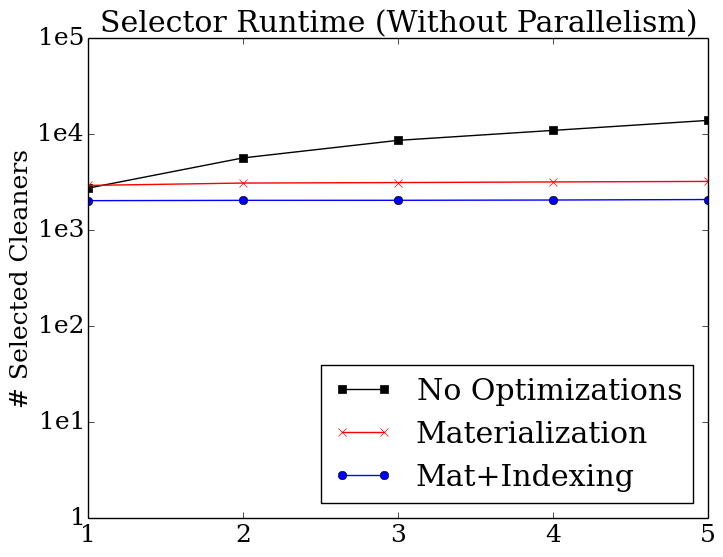
\includegraphics[width=0.8\columnwidth]{exp/opt1.png}
 \caption{This plot (log scale) shows the impact of optimizations on the selector's runtime. Materialization and Indexing allow the algorithm to scale with the number of selected cleaners. Otherwise, the algorithm repeatedly retrains and recleans the same data.
 \label{fig:opt}}
\end{figure}
 
 \subsubsection{Repair Selector Optimizations}
 Next, we evaluate the selector optimizations. We proposed two systems optimizations to the boosting algorithm: (1) materialization, and (2) indexing.
 In this set of experiments, we use FEC dataset and apply no parallelism.
 Figure \ref{fig:opt} plots the runtime of the repair selector as a function of the number of cleaners to select (i.e., B).
 Without any optimization, for $B=1$ the repair selector requires 2754 seconds and for $B=5$ requires 14002 seconds.
 The materialization optimization allows us to pay an up-front cost of creating the view during the first iteration of the algorithm, but saves effort on future iterations.
 For $B=1$ with the materialization optimization, the run time is 2943 seconds.
 For $B=5$ the time is drastically cut down to 3241 seconds.
 In each iteration, the indexing algorithm allows us to more efficiently evaluate the accuracy of a cleaner+classifier pair.
 This reduces the run time at $B=5$ to 2072.
 
 \begin{figure}[t]
\centering
 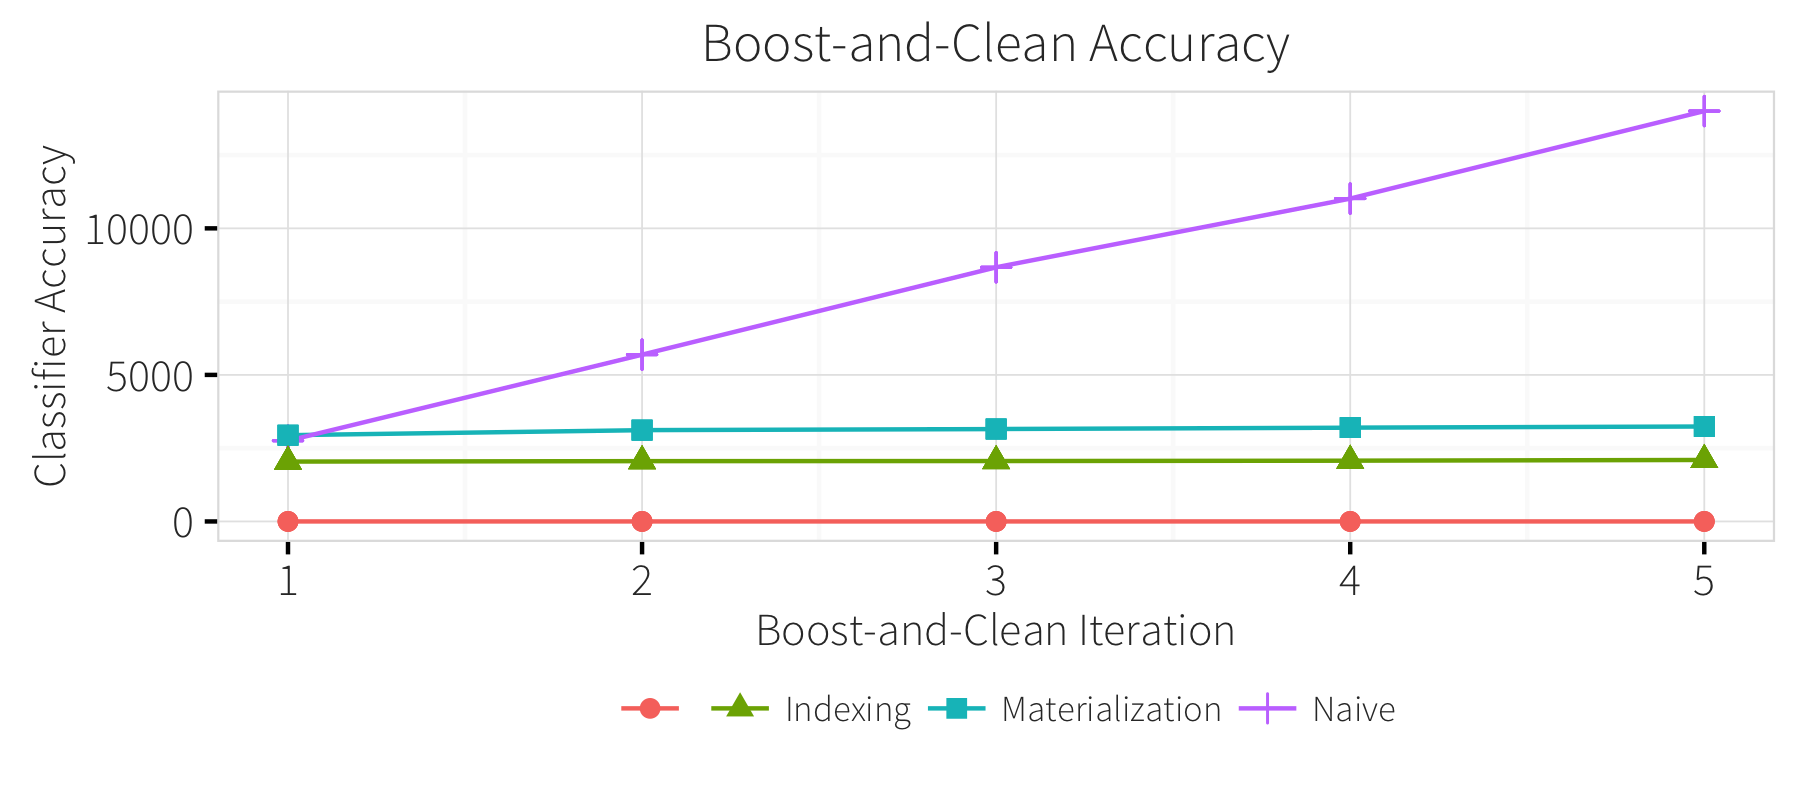
\includegraphics[width=0.8\columnwidth]{exp/learn.png}
 \caption{For three different classification models, we plot the learning curves for the repair selector. Selecting too many cleaners can lead to overfitting.
 \label{fig:learning}}
\end{figure}
 
 \subsubsection{Repair Selector Overfitting}
 One concern with the repair selector is overfitting. We evaluate to what extent, \sys overfits in Figure \ref{fig:learning}, where we plot the learning curves (accuracy as a function of the number of cleaners $B$).
 We try three different classification models, random forests, SVMs, and logistic regression.
 For all of the models we see similar results, where there is an optimal $B$ to select after which \sys overfits.
This is a major concern on small datasets \ewu{How Small?}, but for a sufficiently large dataset with proper test and training evaluation, this can be set through cross-validation. 

\subsubsection{Synthetic Corruptions}

 



\section{Related Work}
There is a growing body of literature that studies analysis-driven data cleaning, that is, applying data cleaning in a sufficient way to answer a given query.
For example, Altwaijry et al.~\cite{altwaijry2015query} describe a technique for resolving a sufficient subset of entities in a database to answer SPJ queries.
Bergman et al. \cite{DBLP:conf/sigmod/BergmanMNT15} proposed identifying errors in selection query results and generating crowd-scoured queries to determine fixes to the base data.
Similarly, work on the consistent query answering problem explored the minimal effort needed to answer a query given a set of integrity constraints over a dirty relation~\cite{DBLP:series/synthesis/2011Bertossi}.

While the work on relational queries is extensive, analytical queries (aggregates, advanced statistical analytics, learning etc.) is less studied.
Projects like ActiveClean~\cite{DBLP:journals/pvldb/KrishnanWWFG16} have studied algorithms for prioritizing user-defined cleaning using the downstream ML model, ActiveClean does not actually clean the data--it only decides where to apply a predefined operation.
\sys studies an extension where the cleaning operations can be selected from a discrete set given a clean test dataset (can be much smaller) to evaluate the user's analytics.
This approach promises to significantly reduce the effort in designing cleaning software since the time-consuming trial-and-error development process is automated.

Furthermore, there are alternative ensembling approaches that could be considered like Multi-Arm Bandits~\cite{bubeck2013multiple}. 
In our particular problem statement, we assume a fixed test set.
This means that the problem is deterministic unlike the bandit setting.
Furthermore, we are interested in selecting a subset that jointly maximizes prediction accuracy and not a top-k.
We hope to explore this avenue in the future and this might be promising for ``weak'' accuracy metrics.

There are a number of other works that use machine learning to improve the efficiency and/or reliability of data cleaning~\cite{DBLP:journals/pvldb/YakoutENOI11,yakout2013don,gokhale2014corleone}.
For example, Yakout et al. train a model that evaluates the likelihood of a proposed replacement value \cite{yakout2013don}.
Another application of machine learning is value imputation, where a missing value is predicted based on those records without missing values.
Machine learning is also increasingly applied to make automated repairs more reliable with human validation \cite{DBLP:journals/pvldb/YakoutENOI11}.
Human input is often expensive and impractical to apply to entire large datasets.
Machine learning can extrapolate rules from a small set of examples cleaned by a human (or humans) to uncleaned data \cite{gokhale2014corleone, DBLP:journals/pvldb/YakoutENOI11}.
This approach can be coupled with active learning \cite{DBLP:journals/pvldb/MozafariSFJM14} to learn an accurate model with the fewest possible number of examples.
While, in spirit, \sys is similar to these approaches, it addresses a very different problem of data cleaning optimization for user-defined ML-based analytics.



 \section{Conclusion and Future Work}
We have shown that automated data cleaning for predictive models can be cast in a statistical boosting framework.  We have prototyped this idea in \sys, a new data cleaning system that detects errors in ML data and uses knowledge of the labels to adaptively select from a set of repair actions to maximize prediction accuracy.
We evaluated results on 8 ML datasets on Kaggle and the UCI repository with real data errors and compare to statistical anomaly detection techniques, constraint-based techniques, and the best single cleaner performance. In all 8 datasets, \sys increased the  test accuracy over alternatives. In addition, we evaluated \sys on production datasets from a data science company and showed that, despite high class imbalances in both datasets, \sys can automatically detect data errors and improve the AUC of the downstream model by $8-9\%$.  We also demonstrate how our optimizations can achieve an end-to-end speed up of over $22\times$

%can parallelize the inner-loop of the boosting operation, and on a 16-core machine \sys achieves a 9.7x speedup. Similarly, we show that building an inverted index can speed up operator selection time by 2.3x.

We are excited about these promising results and have identified a number of future research directions to improve the practicality of the system.  The first is to relax the current requirements of having a test set with clean labels.   Although it may be difficult to acquire sufficient test labels, data science application often have access to an indirect model accuracy measure.  For instance, user retention may be strongly correlated to model accuracy and much easier to obtain.  This will likely require a more complex ensembling technique than boosting.  A second direction is to support parameterized cleaning operations, such as regular expression extractors, for which the number of possible parameter values is unbounded.  We believe that recursive discretization procedures are a promising approach.  A third direction are further performance optimizations so that \sys can scale to large and heterogeneous settings such as data lakes.  Finally, we are actively seeking to continue industrial collaborations and real-world evaluations of our system.  The system and code is open source and can be accessed at {\bf anonymized for submission.}


% \input{impestimate.tex}

%\input{optimizer.tex}
%\section{Experiments}\label{s:exp}
In this section, we present the results of our experiments.  We execute \sys on $13$ datasets based on three sets of real-world cases---machine learning competitions, data analysis pipelines, and \company---and report accuracy measures and end-to-end runtime.  Then, we present a series of micro-benchmarks that evaluate each of the modules of \sys.  Our goal is to understand the conditions where automated cleaning is able to accurately detect and repair data in a way that improves the held-out test accuracy.

\subsection{Baselines and Methods}
To the best of our knowledge, there does not exist a comparable general purpose ML+Data Cleaning system to \sys in industry or academia.
We evaluate \sys against a number of baseline approaches inspired by solutions proposed in literature. 

\vspace{0.25em}\noindent\textbf{No Cleaning (NC): } We train a model without any modification to the training or test data.

\vspace{0.25em}\noindent\textbf{Quantitative (Q): } We train a model where only quantitative outliers in both training and test are imputed with a mean value. \ewu{Are outliers detected using isolation forest + numerical attribute featurizer?} 

\vspace{0.25em}\noindent\textbf{Integrity Constraint (IC): } We read through each dataset to identify a set of anomalous values for each attribute on a best-effort basis.  We then codified these as integrity constraint rules, and corrected the identified errors using a statistical distortion minimization metric as in~\cite{prokoshyna2015combining}.\ewu{  In one sentence what is the statistical distortion min metric}

\vspace{0.25em}\noindent\textbf{Quantitative + IC (Q+IC): } We use the quantitative and integrity constraints for detection; we use mean and mode imputation as repair functions for numerical and text attributes, respectively.

\vspace{0.25em}\noindent\textbf{Best Single (Best-1): } We run \sys with $B=1$ and identify the  single best conditional repair.

\vspace{0.25em}\noindent\textbf{Worst Single (Worst-1): } We run \sys with $B=1$ and identify the single worst conditional repair..

\stitle{BC-3: } We run \sys with $B=3$.

\stitle{BC-5: } We run \sys with $B=5$.


\vspace{0.25em}

\ewu{NEED TO EXPLAIN WHAT TEST DATASET IS.}


In all of our experiments, we used standard classification models and featurization techniques from Python \textsf{sklearn}.
The classifiers were trained in Python 2.7 and timing experiments were run on an Amazon EC2 m4.16xlarge instance\footnote{64 virtual cpus and 256 GiB memory}.
To avoid overfitting, we carefully designed the accuracy evaluation experiments for \sys by using a ``doubly'' held out test dataset: the test dataset used to optimize \sys is different from a completely unseen test dataset that is solely used to report the final prediction accuracy.
We describe hyper-parameter settings for each technique in the text of each experiment.

We used the \textsf{sklearn} Random Forest classifier with custom depth and branch parameters.  The training procedure uses a set of standard featurizers (hot-one encoding for categorical data, bag-of-words for string data, numerical data as is) in a similar fashion as~\cite{DBLP:conf/sigmod/GokhaleDDNRSZ14}.  Note that these featurizers are used as part of the black-box training procedure and are distinct from those used in the detector generator library.




\begin{table*}[t]
\centering
\label{tab:accuracy}
\begin{tabular}{|l|r|r|r|r|r|r|r|r|r|}
\hline
ML Competition& NC & Q &	IC & Q+IC &	Best-1 &	Worst-1 &	BC-3 & BC5 & Rel. Improvement\\
\hline
USCensus	&0.85&	0.82&	0.86&	0.84&	0.87&	0.79&	0.88&	\blue{0.91} & +4.5\% \\
Emergency &	0.67&	0.72&	0.67&	0.72&	0.72&	0.66&	0.72&	\blue{0.75} & +4.7\%\\
Sensor	&0.92&	0.93&	0.92&	0.89&	0.92&	0.8&	\blue{0.94}&	0.94 & +1.3\%\\
NFL	&0.74&	0.74&	0.76&	0.75&	0.76&	0.74&	0.79&	\blue{0.82}& +5.1\%\\
EEG	&0.79&	0.82&	0.79&	0.83&	0.83&	0.7&	0.85&	\blue{0.89}& +6.8\%\\
Titanic	&0.83&	0.72&	0.83&	0.76&	0.83&	0.69&	0.83&	\blue{0.84}& +1.1\%\\
Housing	&0.73&	0.76&	0.73&	0.77&	0.77&	0.65&	\blue{0.81}&	0.76& +5.1\% \\
Retail	&0.88&	0.88&	0.91&	0.91&	0.91&	0.87&	0.94&	\blue{0.95}& +4.3\% \\
\hline
\hline
Data Analytics & NC & Q &	IC & Q+IC &	Best &	Worst &	BC-3 & BC5 & Rel. Improvement\\
\hline
FEC  & 0.62 & 0.53 & 0.61 & 0.57 & 0.71 & 0.51 & 0.74 & \blue{0.77} &  +8.4\% \\
Restaurant (Multiclass) & 0.42 & 0.42 & 0.58 & 0.68 & \blue{0.62} & 0.36 & 0.61 & 0.60 & (1.61)\% \\
\hline
\hline
Company X & NC & Q &	IC & Q+IC &	Best &	Worst &	BC-3 & BC5 & Rel. Improvement\\
\hline
Dataset 1 (AUC) &0.60& & & &0.61& & &0.66& 0.69\\
Dataset 2 & & & & & & & & &\\
Dataset 3 & & & & & & & & &\\
\hline
\end{tabular}
\caption{End-to-end accuracy results for each dataset and experimental method. We report standard classification accuracy.  The right column summarizes the accuracy improvement relative to the best non BC-3/5 approach.}
\end{table*}


\subsection{End-to-End Accuracy}
In our first experiment, we evaluated the accuracy of \sys compared to the baselines.
We tried to minimize hyper-parameter tuning as much as possible to simulate a real-scenario where extensive tuning and parameter search might be expensive.


\subsubsection{ML Competition Datasets}\label{exp:comp}
We downloaded 8 binary classification datasets from Kaggle competitions and benchmarks in the UCI ML repository.  \ewu{The next two sentences seem contradictory: they are clean, but dirty} These datasets are mostly clean as they have been extracted, structured, and published.
Nevertheless, they contain missing values, numerical outliers, and pattern errors (oddly formatted values).
For this set of experiments, we used a single hyper-parameter setting for all the detectors and classification models (default \textsf{sklearn} library setting). \ewu{IMPORTANT: SOMEWHERE IN THE WRITING, WE FORGOT TO TALK ABOUT HYPERPARAMETERS}

We briefly describe each dataset and their errors below:

\vspace{0.5em}\noindent\textbf{USCensus: } This dataset contains US Census records for adults and the goal is to predict  whether the adult earns more than $50,000$ dollars. It contains 32,561 records with 15 numerical and categorical attributes. Examples of data error include:
\begin{lstlisting}
#missing values
40,Private,121772,Assoc-voc,11,
Married-civ-spouse,Craft-repair,Husband, 
Asian-Pac-Islander,Male,0,0,40,(*\orange{\bf{?}}*),>50K

#coding inconsistency
57,Local-gov,110417,HS-grad,9,
Married-civ-spouse,Craft-repair,Husband,
White,Male,(*\orange{\bf{99999}}*),0,40,United-States,>50K
\end{lstlisting}

\vspace{0.5em}\noindent\textbf{NFL: } This dataset contains play-by-play logs from US Football games. The dataset contains 46,129 records with 65 numerical, categorical, and string-valued attributes. Given the record, the classification objective is to determine whether the next play the team runs is a run or a pass play.
The dataset contains a significant number of missing values and ``sentinel'' records that mark the end of a log sequence:\ewu{What distinguishes a sentinel?}
\begin{lstlisting}
#missing values
"36",2015-09-10,"2015091000",1,1,(*\orange{\bf{NA}}*),"15:00",
15,3600,0,"NE",35,35,0,0,0,(*\orange{\bf{NA}}*),"PIT","NE"(*\blue{\bf{....}}*)

#sentinel record
"189710",2016-01-03,"2016010310",10,2,NA,"00:00",
0,1800,8,"GB",17,17,0,-1,0,0,"",NA,"END(*~*)QUARTER2"
,1,0,0,0,NA, NA,NA,0,"Quarter(*~*)End"(*\blue{\bf{....}}*)
\end{lstlisting}

\vspace{0.5em}\noindent\textbf{EEG: } This dataset contains \ewu{SANJAY DESCRIBE}
\begin{lstlisting}

\end{lstlisting}

\vspace{0.5em}\noindent\textbf{Emergency: } This dataset contains records on 911 calls from Pennsylvania. There are 111,766 records with 9 attributes. Given the record, the classification challenge is to determine whether the emergency service response time will be less than $5 min$. This dataset contains missing values, and spurious locations not served by the 911 center:
\begin{lstlisting}
#missing values
41.1671565,-76.8740304,MAIN;(*\orange{\bf{--}}*); Station 308A;
2016-01-02 @ 13:01:30;,17752,EMS: UNKNOWN MEDICAL
EMERGENCY,2016-01-02 13:06:00,(*\orange{\bf{--}}*),MAIN,1

#spurious location (outisde 100 mile radius)
(*\orange{\bf{41.1671565,-76.8740304,}}*)MAIN;(*\orange{\bf{--}}*); Station 308A;
2016-01-02 @ 13:01:30;,17752,EMS: UNKNOWN MEDICAL 
EMERGENCY,2016-01-02 13:06:00,(*\orange{\bf{--}}*),MAIN,1
\end{lstlisting}

\vspace{0.5em}\noindent\textbf{Sensor: } The Intel sensor dataset~\cite{} contains 928,991 temperature, humidity, and light sensor readings a sensor deployment. The classification task is to predict whether the readings came from a particular sensor (sensor 49). This dataset has numerical outliers:
\begin{lstlisting}
#Normal Record
49  -0.999750  12.862100  10.368300  10.438300  
11.669900 (*\orange{\bf{13.493100}}*)  13.342300  8.041690  
8.739010  26.225700  59.052800

#Spurious Record
49  1.175188  12.279100  8.849360  9.005830  
10.111700  (*\orange{\bf{378.750000}}*)  19.319400  15.916200  
37.631400  27.150100  53.403700
\end{lstlisting}

\vspace{0.5em}\noindent\textbf{Titanic: } This dataset contains 891 records from the Titanic manifest with 12 attributes. The classification objective is to determine whether the passenger survived or not. There are missing values and string formatting errors:

\begin{lstlisting}
#missing values
891,0,3,"Dooley, Mr. Patrick",male,
32,0,0,370376,7.75,(*\orange{\bf{--}}*),Q
\end{lstlisting}

\vspace{0.5em}\noindent\textbf{Housing: } The housing dataset contains 1460 records and 81 attributes of house price listings. The classification objective is to determine whether the listed house will be sold above 750000. 
This dataset contains missing values as well as numerical outliers:
\begin{lstlisting}
#missing values
(*\blue{\bf{....}}*)204,228,0,0,0,(*\orange{\bf{NA,NA}}*),Shed,350,11,2009,WD,
Normal,200000
\end{lstlisting}

\vspace{0.5em}\noindent\textbf{Retail: } The online retail dataset contains 541,909 records of online retail purchases with 8 attributes. The classification objective is to predict whether the purchase occurred in the United Kingdom.
This dataset contains numerical errors where some purchased quantities are reported as negative:
\begin{lstlisting}
#outliers
C536391,21980,PACK OF 12 RED RETROSPOT TISSUES
,(*\orange{\bf{-24}}*),12/1/10 10:24,0.29,17548,United Kingdom
\end{lstlisting}

\vspace{1em}
The first set of rows in Table \ref{tab:accuracy} present the predictive accuracy of models trained with \sys on the completely unseen test data.  In all experiments, the model trained with one of the \sys  approaches was the most accurate.
The quantitative baseline performed well when the errors were clear numerical outliers (e.g., Sensor and  EEG).  However, its performance suffered in datasets with missing values or formatting errors, and {\it degraded model accuracy} in the US Census dataset.
Conversely, the integrity constraint approach worked well for non-numerical errors, however it was not useful for Emergency, EEG, Housing, nor Sensor.
The naive union of (Q+IC) has difficulty composing the two operations in the US Census dataset and degrades accuracy as compared to quantitative or integrity constraint alone in several datasets.  Finally we compare and find up to a 14\% difference between the best and worst repairs when using \sys.  These results emphasize the need for an automatic search solution that can avoid repairs that are ineffective or reduce accuracy.

\ewu{What about BC3 and BC5}


\subsubsection{Data Analytics}
The next class of datasets that we considered were datasets known to have significant errors--unlike the relatively clean competition datasets. These are two datasets that were used in previous data cleaning papers, and we designed classification tasks based on the datasets.
Unlike the ML competition datasets, we tuned the classifier and detector hyperparamters for each dataset. 
The accuracy results are presented in the second set of rows in Table \ref{tab:accuracy}.

\vspace{0.5em}\noindent\textbf{Federal Election Commission Contributions: } The FEC provides a dataset of election contributions of 6,410,678 records with 18 numerical, categorical and string valued attributes. This dataset has a number of errors. There are missing values, formatting issues (where records have the wrong number of fields causing misaligment in parsing), and numerical outliers (negative contributions).

\begin{lstlisting}
#missing values
C00458844,"P60006723","Rubio, Marco","RUCINSKI,
ROBERT","APO","AE","090960009","US ARMY",
"PHYSICIAN",100,08-MAR-16,(*\orange{\bf{``''}}*),(*\orange{\bf{``''}}*),(*\orange{\bf{``''}}*),"SA17A",
"1082559","SA17.1074981","P2016"

#misalignment
C00458844, "P60006723", (*\orange{\bf{"Rubio", "Marco"}}*), "BRIZOLIS",
" DEMETRI MR.", "RANCHO SANTA FE", "CA", 
"920674357", "RETIRED", "RETIRED", 100, 
28-OCT-15, "", "", "", "SA17A", "1047126", 
"SA17.851920", "P2016"

#rejected contributions double recorded
C00458844,"P60006723","Rubio, Marco","SWAID, 
SWAID N. DR.","BIRMINGHAM","AL","352660827",
"NEWOLOGICAL SURGERY ASSOCIATES","PHYSICIAN",
(*\orange{\bf{-400}}*),28-DEC-15, "REDESIGNATION TO GENERAL","X",
"REDESIGNATION TO GENERAL","SA17A",
"1047126","SA17.892835B","P2016"

C00458844,"P60006723","Rubio, Marco","SWAID, 
SWAID N. DR.","BIRMINGHAM","AL","352660827",
"NEWOLOGICAL SURGERY ASSOCIATES","PHYSICIAN",
(*\orange{\bf{400}}*),28-DEC-15, 
"REDESIGNATION FROM PRIMARY","X", 
"REDESIGNATION FROM PRIMARY","SA17A",
"1047126","SA17.918421","G2016"
\end{lstlisting}

Our classification objective was to determine whether the contribution would be above or below $100$ dollars. Due to the severity of the errors in the dataset, there is nearly a 15\% difference between the prediction accuracy of a classifier with and without \sys.
Furthermore, a purely quantitative approach is not useful for this dataset.
An integrity constraint based method improves accuracy but the automatic imputations are unreliable on this data.
Furthermore, it is difficult to express a problem like row misalignment as a integrity constraint.

We find empirically that the alignment is better detected by the word2vec error detector in \sys.
As a result the best single cleaner is using the word2vec error detector.
This is improved by combining this with quantitative checks for numerical outliers and missing values.
In all, \sys with a budget of 5 improves accuracy 8.4\% over the best single cleaner. 

\vspace{0.5em}\noindent\textbf{Restaurant Dataset: } The restaurant dataset has 758 distinct records and 4 attributes. This dataset has typically been used as a benchmark for entity resolution since records are duplicated with minor inconsistencies.
We designed a multi-class classification task to see if we could predict the city from record.
One of the major inconsistencies was additional attributes appended to the restaurant category.

\begin{lstlisting}
campanile,624 s. la brea ave.,los angeles,
american

grill  the,9560 dayton way,beverly hills,
american (*\orange{\bf{(traditional)}}*)
\end{lstlisting}

On this dataset, we see a negative result from \sys. Our test error decreases as we increase the number of selected cleaners. We speculate this is due to overfitting due to the extremely small size of the dataset  ($<1000 records$) combined with the expressiveness of the classifiers model.

\subsubsection{Company X Experiments}
We applied \sys to three datasets from Company X.

\reminder{TODO Write Description}

\begin{figure}[t]
\centering
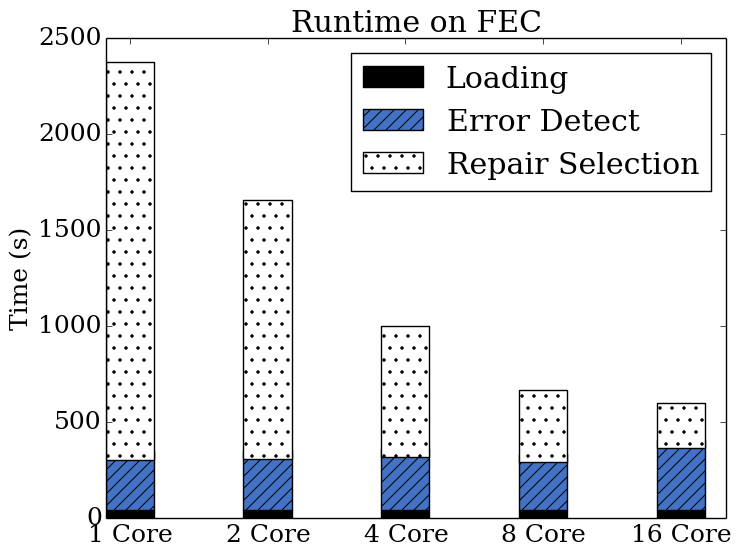
\includegraphics[width=0.8\columnwidth]{exp/runtime.png}
\caption{(A) This plot measures the run-time on a 6M record dataset (1.5GB) grouped by the number of cores on the machine. The repair selection scales but the other steps are not parallelized.\label{exp:runtime}}
\end{figure}

\begin{figure}[t]
\centering
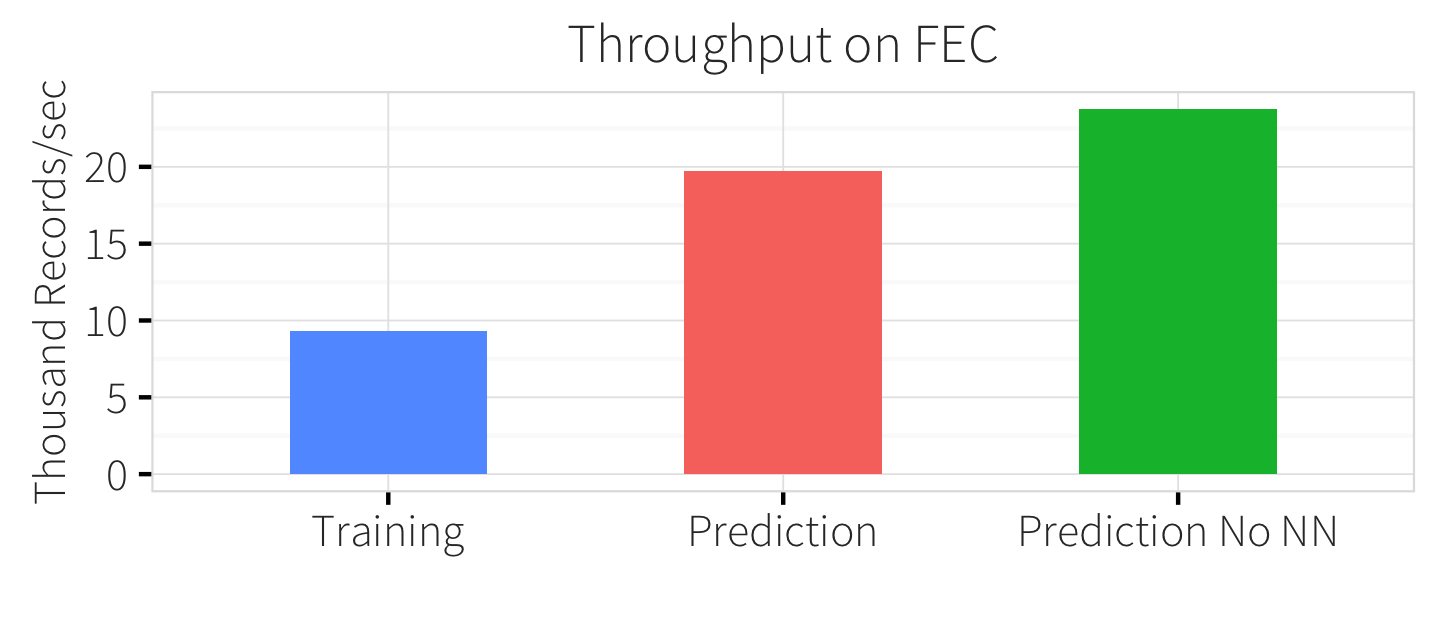
\includegraphics[width=0.8\columnwidth]{exp/runtime2.png}
\caption{We plot the prediction and training throughput for 16-cores. Prediction throughput is much higher than training throughput.\label{exp:tp}}
\end{figure}

\subsection{End-to-End Run Time}
Next, we evaluate the end-to-end wall clock runtime of \sys. We use the FEC dataset since it is the largest. This evaluation includes all of the optimizations for \sys. The FEC dataset is 1.5 GB (about 6M records). 
Figure \ref{exp:runtime} plots the results.
With a single core, \sys takes 2422 seconds in wall-clock time. Of that time, 2072 seconds is spent in repair selection, 306 seconds is spent in error detection, and 44 seconds in loading the dataset.
We can parallelize the repair selection step. We parallelize the inner-loop of the boosting algorithm. On 16-cores, we are able to reduce the runtime of the repair selection to 212 seconds. This constitutes a 9.7x speedup for that step.

It is important to note that this latency is only incurred during training. During prediction, the learned model can be applied, and this process is much faster than training. 
Figure \ref{exp:tp} plots the throughput of \sys.
The number of records that can be processed per second on 16 cores for prediction is 19746 records/second, but during training it is 9316 records/second. One of the key bottlenecks is evaluating the word2vec model for each prediction, and without this model, the throughput increases to 23746 records/second.

\begin{figure}[t]
\centering
 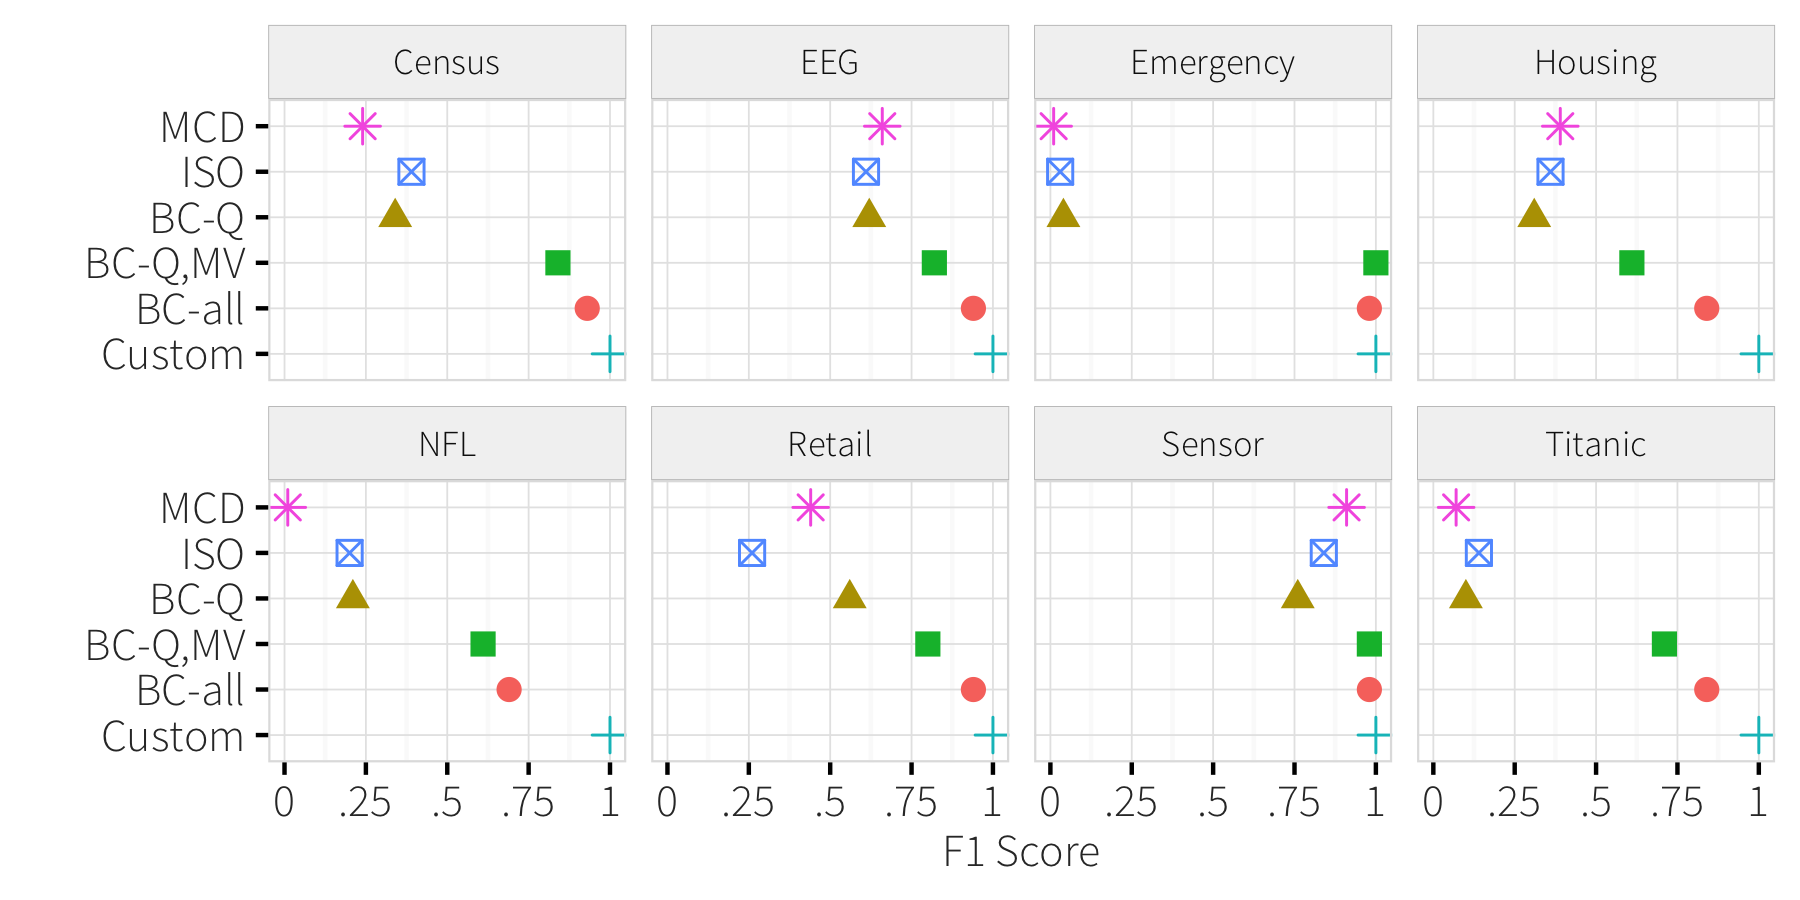
\includegraphics[width=\columnwidth]{exp/daccuracy.png}
 \caption{On 8 Machine Learning competition datasets, we evaluated the F1 accuracy score of different error detection techniques. We compare against Isolation Forest (alone), Minimum Covariance Determinants, and Hand-Written rules. We evaluate \sys using only the Isolation forest for numerical outliers, outliers+missing values, and outliers+missing values+word2vec.
 The final detector in \sys achieves up to 81\% of the accuracy on the competition datasets.
 \label{fig:derror}}
\end{figure}

\begin{figure}[t]
\centering
 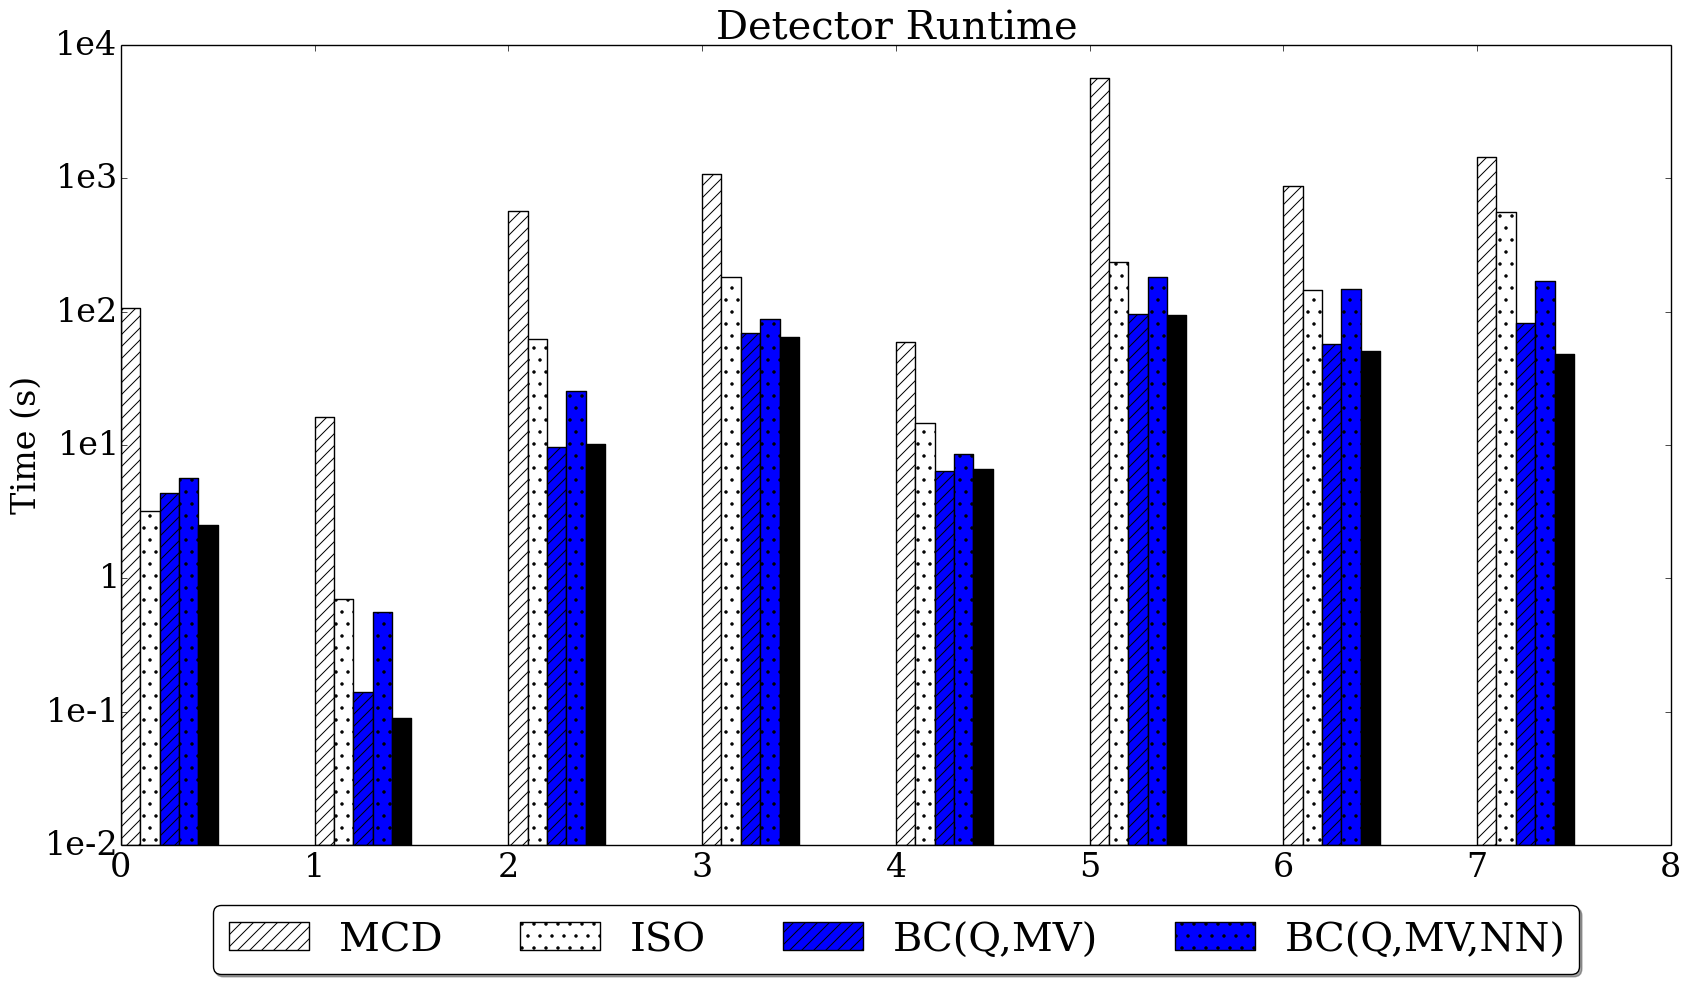
\includegraphics[width=\columnwidth]{exp/druntime.png}
 \caption{On 8 Machine Learning competition datasets, we evaluated the runtime of each of the detection methods. We compare against Isolation Forest, Minimum Covariance Determinants, and Hand-Written rules. While evaluating hand-written rules is certainly faster, \sys is faster in terms of wall-clock time than MCD.
 \label{fig:druntime}}
\end{figure}

\subsection{Micro-Benchmarks}
Next, we evaluate the different components of \sys in terms of accuracy and runtime.

\subsubsection{Detectors}
The first component that we evaluate are the detectors. We design a set of automatic error detectors based on heuristics, statistical criteria, and the word2vec neural network. We first measure its accuracy against hand-written detection scripts, and other quantitative outlier detection techniques (Isolation Forests and Minimum Covariance Determinants).
\sys internally uses an Isolation Forest combined with other error detectors, so we evaluate \sys with and without certain detection modules.
We measure accuracy w.r.t the alternatives with the F1 accuracy measure.

 Figure  \ref{fig:derror} shows that the final detector in \sys achieves up to 81\% of the accuracy of hand-written rules on the competition datasets.
Confirming the results of Abedjan et al.~\cite{DBLP:journals/pvldb/AbedjanCDFIOPST16}, we found that a 
purely quantitative approach does not perform well in comparison to the rule-based approach on these datasets (Isolation Forest alone and MCD).
However, results are significantly improved when combined with heuristics that detect missing values. 
The performance gap is even further reduced when the detector additionally uses a Neural Network to learn how attributes correlate with each other, and detect anomolous correlations.
It is important to emphasize that these datasets represent a very specific domain, i.e., structured training datasets for ML.
The datasets are already in a structured schema and the only thing that an analyst has to worry about is handling inconsistent attribute values.
Presumably these datasets were also previously cleaned and extracted before they were publicly released.
Our initial experiment showed that for this class of datasets, reasonably accurate error detection is possible with minimal supervision and tuning.

 Figure  \ref{fig:druntime} shows the runtime of each of the approaches.
 We found that MCD was a very expensive quantitative error detection approach (orders of magnitude slower).
 This was one of the big motivations for using an isolation forest internally in \sys.
 Of course, rules are faster to evaluate than a learning detector and this gap was on average a factor of 3.
 
 \begin{figure}[t]
\centering
 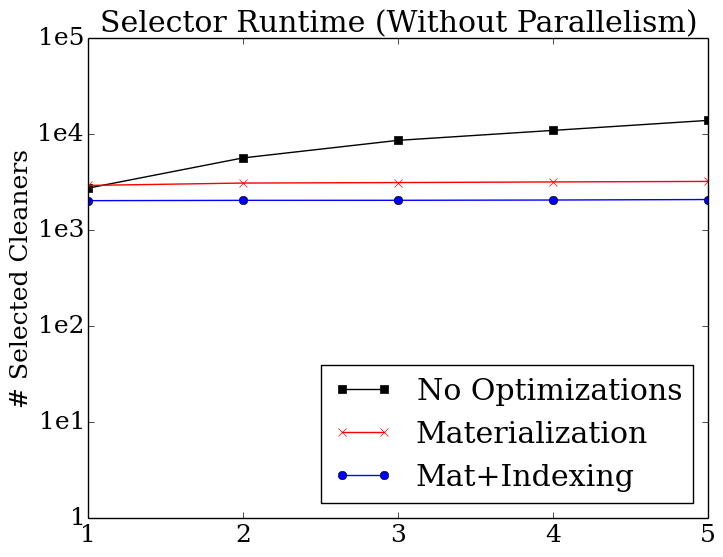
\includegraphics[width=0.8\columnwidth]{exp/opt1.png}
 \caption{This plot (log scale) shows the impact of optimizations on the selector's runtime. Materialization and Indexing allow the algorithm to scale with the number of selected cleaners. Otherwise, the algorithm repeatedly retrains and recleans the same data.
 \label{fig:opt}}
\end{figure}
 
 \subsubsection{Repair Selector Optimizations}
 Next, we evaluate the selector optimizations. We proposed two systems optimizations to the boosting algorithm: (1) materialization, and (2) indexing.
 In this set of experiments, we use FEC dataset and apply no parallelism.
 Figure \ref{fig:opt} plots the runtime of the repair selector as a function of the number of cleaners to select (i.e., B).
 Without any optimization, for $B=1$ the repair selector requires 2754 seconds and for $B=5$ requires 14002 seconds.
 The materialization optimization allows us to pay an up-front cost of creating the view during the first iteration of the algorithm, but saves effort on future iterations.
 For $B=1$ with the materialization optimization, the run time is 2943 seconds.
 For $B=5$ the time is drastically cut down to 3241 seconds.
 In each iteration, the indexing algorithm allows us to more efficiently evaluate the accuracy of a cleaner+classifier pair.
 This reduces the run time at $B=5$ to 2072.
 
 \begin{figure}[t]
\centering
 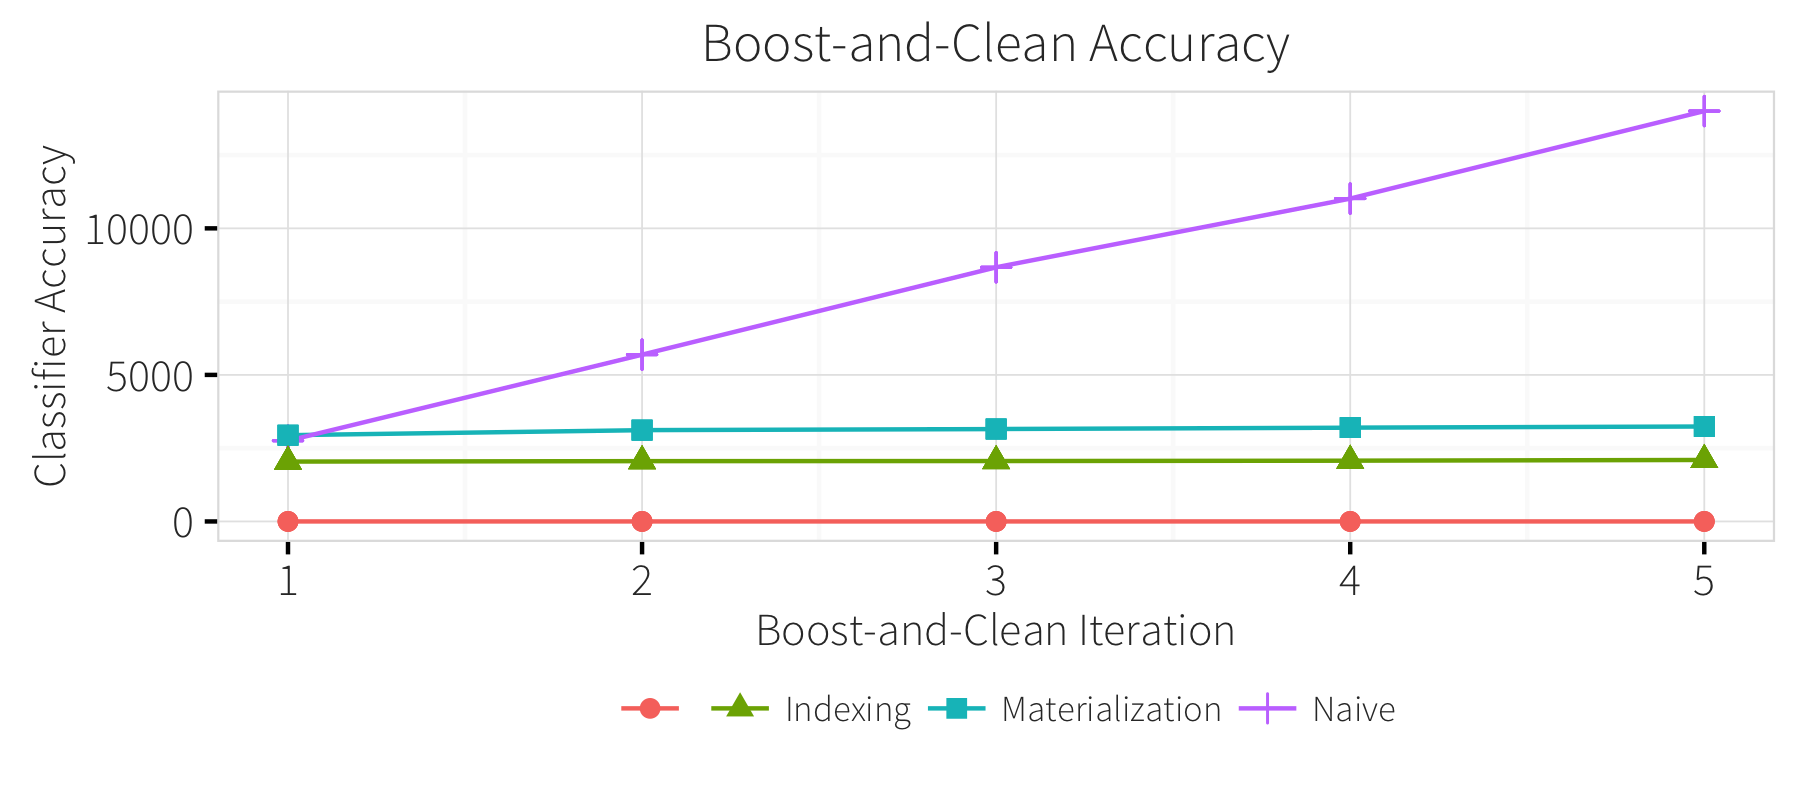
\includegraphics[width=0.8\columnwidth]{exp/learn.png}
 \caption{For three different classification models, we plot the learning curves for the repair selector. Selecting too many cleaners can lead to overfitting.
 \label{fig:learning}}
\end{figure}
 
 \subsubsection{Repair Selector Overfitting}
 One concern with the repair selector is overfitting. We evaluate to what extent, \sys overfits in Figure \ref{fig:learning}, where we plot the learning curves (accuracy as a function of the number of cleaners $B$).
 We try three different classification models, random forests, SVMs, and logistic regression.
 For all of the models we see similar results, where there is an optimal $B$ to select after which \sys overfits.
This is a major concern on small datasets \ewu{How Small?}, but for a sufficiently large dataset with proper test and training evaluation, this can be set through cross-validation. 

\subsubsection{Synthetic Corruptions}

 



%\section{Related Work}
There is a growing body of literature that studies analysis-driven data cleaning, that is, applying data cleaning in a sufficient way to answer a given query.
For example, Altwaijry et al.~\cite{altwaijry2015query} describe a technique for resolving a sufficient subset of entities in a database to answer SPJ queries.
Bergman et al. \cite{DBLP:conf/sigmod/BergmanMNT15} proposed identifying errors in selection query results and generating crowd-scoured queries to determine fixes to the base data.
Similarly, work on the consistent query answering problem explored the minimal effort needed to answer a query given a set of integrity constraints over a dirty relation~\cite{DBLP:series/synthesis/2011Bertossi}.

While the work on relational queries is extensive, analytical queries (aggregates, advanced statistical analytics, learning etc.) is less studied.
Projects like ActiveClean~\cite{DBLP:journals/pvldb/KrishnanWWFG16} have studied algorithms for prioritizing user-defined cleaning using the downstream ML model, ActiveClean does not actually clean the data--it only decides where to apply a predefined operation.
\sys studies an extension where the cleaning operations can be selected from a discrete set given a clean test dataset (can be much smaller) to evaluate the user's analytics.
This approach promises to significantly reduce the effort in designing cleaning software since the time-consuming trial-and-error development process is automated.

Furthermore, there are alternative ensembling approaches that could be considered like Multi-Arm Bandits~\cite{bubeck2013multiple}. 
In our particular problem statement, we assume a fixed test set.
This means that the problem is deterministic unlike the bandit setting.
Furthermore, we are interested in selecting a subset that jointly maximizes prediction accuracy and not a top-k.
We hope to explore this avenue in the future and this might be promising for ``weak'' accuracy metrics.

There are a number of other works that use machine learning to improve the efficiency and/or reliability of data cleaning~\cite{DBLP:journals/pvldb/YakoutENOI11,yakout2013don,gokhale2014corleone}.
For example, Yakout et al. train a model that evaluates the likelihood of a proposed replacement value \cite{yakout2013don}.
Another application of machine learning is value imputation, where a missing value is predicted based on those records without missing values.
Machine learning is also increasingly applied to make automated repairs more reliable with human validation \cite{DBLP:journals/pvldb/YakoutENOI11}.
Human input is often expensive and impractical to apply to entire large datasets.
Machine learning can extrapolate rules from a small set of examples cleaned by a human (or humans) to uncleaned data \cite{gokhale2014corleone, DBLP:journals/pvldb/YakoutENOI11}.
This approach can be coupled with active learning \cite{DBLP:journals/pvldb/MozafariSFJM14} to learn an accurate model with the fewest possible number of examples.
While, in spirit, \sys is similar to these approaches, it addresses a very different problem of data cleaning optimization for user-defined ML-based analytics.



%\input{discussion.tex}
%\section{Conclusion and Future Work}
We have shown that automated data cleaning for predictive models can be cast in a statistical boosting framework.  We have prototyped this idea in \sys, a new data cleaning system that detects errors in ML data and uses knowledge of the labels to adaptively select from a set of repair actions to maximize prediction accuracy.
We evaluated results on 8 ML datasets on Kaggle and the UCI repository with real data errors and compare to statistical anomaly detection techniques, constraint-based techniques, and the best single cleaner performance. In all 8 datasets, \sys increased the  test accuracy over alternatives. In addition, we evaluated \sys on production datasets from a data science company and showed that, despite high class imbalances in both datasets, \sys can automatically detect data errors and improve the AUC of the downstream model by $8-9\%$.  We also demonstrate how our optimizations can achieve an end-to-end speed up of over $22\times$

%can parallelize the inner-loop of the boosting operation, and on a 16-core machine \sys achieves a 9.7x speedup. Similarly, we show that building an inverted index can speed up operator selection time by 2.3x.

We are excited about these promising results and have identified a number of future research directions to improve the practicality of the system.  The first is to relax the current requirements of having a test set with clean labels.   Although it may be difficult to acquire sufficient test labels, data science application often have access to an indirect model accuracy measure.  For instance, user retention may be strongly correlated to model accuracy and much easier to obtain.  This will likely require a more complex ensembling technique than boosting.  A second direction is to support parameterized cleaning operations, such as regular expression extractors, for which the number of possible parameter values is unbounded.  We believe that recursive discretization procedures are a promising approach.  A third direction are further performance optimizations so that \sys can scale to large and heterogeneous settings such as data lakes.  Finally, we are actively seeking to continue industrial collaborations and real-world evaluations of our system.  The system and code is open source and can be accessed at {\bf anonymized for submission.}

%\input{outlier.tex}
%\input{analysis.tex}
%\section{Experiments}\label{s:exp}
In this section, we present the results of our experiments.  We execute \sys on $13$ datasets based on three sets of real-world cases---machine learning competitions, data analysis pipelines, and \company---and report accuracy measures and end-to-end runtime.  Then, we present a series of micro-benchmarks that evaluate each of the modules of \sys.  Our goal is to understand the conditions where automated cleaning is able to accurately detect and repair data in a way that improves the held-out test accuracy.

\subsection{Baselines and Methods}
To the best of our knowledge, there does not exist a comparable general purpose ML+Data Cleaning system to \sys in industry or academia.
We evaluate \sys against a number of baseline approaches inspired by solutions proposed in literature. 

\vspace{0.25em}\noindent\textbf{No Cleaning (NC): } We train a model without any modification to the training or test data.

\vspace{0.25em}\noindent\textbf{Quantitative (Q): } We train a model where only quantitative outliers in both training and test are imputed with a mean value. \ewu{Are outliers detected using isolation forest + numerical attribute featurizer?} 

\vspace{0.25em}\noindent\textbf{Integrity Constraint (IC): } We read through each dataset to identify a set of anomalous values for each attribute on a best-effort basis.  We then codified these as integrity constraint rules, and corrected the identified errors using a statistical distortion minimization metric as in~\cite{prokoshyna2015combining}.\ewu{  In one sentence what is the statistical distortion min metric}

\vspace{0.25em}\noindent\textbf{Quantitative + IC (Q+IC): } We use the quantitative and integrity constraints for detection; we use mean and mode imputation as repair functions for numerical and text attributes, respectively.

\vspace{0.25em}\noindent\textbf{Best Single (Best-1): } We run \sys with $B=1$ and identify the  single best conditional repair.

\vspace{0.25em}\noindent\textbf{Worst Single (Worst-1): } We run \sys with $B=1$ and identify the single worst conditional repair..

\stitle{BC-3: } We run \sys with $B=3$.

\stitle{BC-5: } We run \sys with $B=5$.


\vspace{0.25em}

\ewu{NEED TO EXPLAIN WHAT TEST DATASET IS.}


In all of our experiments, we used standard classification models and featurization techniques from Python \textsf{sklearn}.
The classifiers were trained in Python 2.7 and timing experiments were run on an Amazon EC2 m4.16xlarge instance\footnote{64 virtual cpus and 256 GiB memory}.
To avoid overfitting, we carefully designed the accuracy evaluation experiments for \sys by using a ``doubly'' held out test dataset: the test dataset used to optimize \sys is different from a completely unseen test dataset that is solely used to report the final prediction accuracy.
We describe hyper-parameter settings for each technique in the text of each experiment.

We used the \textsf{sklearn} Random Forest classifier with custom depth and branch parameters.  The training procedure uses a set of standard featurizers (hot-one encoding for categorical data, bag-of-words for string data, numerical data as is) in a similar fashion as~\cite{DBLP:conf/sigmod/GokhaleDDNRSZ14}.  Note that these featurizers are used as part of the black-box training procedure and are distinct from those used in the detector generator library.




\begin{table*}[t]
\centering
\label{tab:accuracy}
\begin{tabular}{|l|r|r|r|r|r|r|r|r|r|}
\hline
ML Competition& NC & Q &	IC & Q+IC &	Best-1 &	Worst-1 &	BC-3 & BC5 & Rel. Improvement\\
\hline
USCensus	&0.85&	0.82&	0.86&	0.84&	0.87&	0.79&	0.88&	\blue{0.91} & +4.5\% \\
Emergency &	0.67&	0.72&	0.67&	0.72&	0.72&	0.66&	0.72&	\blue{0.75} & +4.7\%\\
Sensor	&0.92&	0.93&	0.92&	0.89&	0.92&	0.8&	\blue{0.94}&	0.94 & +1.3\%\\
NFL	&0.74&	0.74&	0.76&	0.75&	0.76&	0.74&	0.79&	\blue{0.82}& +5.1\%\\
EEG	&0.79&	0.82&	0.79&	0.83&	0.83&	0.7&	0.85&	\blue{0.89}& +6.8\%\\
Titanic	&0.83&	0.72&	0.83&	0.76&	0.83&	0.69&	0.83&	\blue{0.84}& +1.1\%\\
Housing	&0.73&	0.76&	0.73&	0.77&	0.77&	0.65&	\blue{0.81}&	0.76& +5.1\% \\
Retail	&0.88&	0.88&	0.91&	0.91&	0.91&	0.87&	0.94&	\blue{0.95}& +4.3\% \\
\hline
\hline
Data Analytics & NC & Q &	IC & Q+IC &	Best &	Worst &	BC-3 & BC5 & Rel. Improvement\\
\hline
FEC  & 0.62 & 0.53 & 0.61 & 0.57 & 0.71 & 0.51 & 0.74 & \blue{0.77} &  +8.4\% \\
Restaurant (Multiclass) & 0.42 & 0.42 & 0.58 & 0.68 & \blue{0.62} & 0.36 & 0.61 & 0.60 & (1.61)\% \\
\hline
\hline
Company X & NC & Q &	IC & Q+IC &	Best &	Worst &	BC-3 & BC5 & Rel. Improvement\\
\hline
Dataset 1 (AUC) &0.60& & & &0.61& & &0.66& 0.69\\
Dataset 2 & & & & & & & & &\\
Dataset 3 & & & & & & & & &\\
\hline
\end{tabular}
\caption{End-to-end accuracy results for each dataset and experimental method. We report standard classification accuracy.  The right column summarizes the accuracy improvement relative to the best non BC-3/5 approach.}
\end{table*}


\subsection{End-to-End Accuracy}
In our first experiment, we evaluated the accuracy of \sys compared to the baselines.
We tried to minimize hyper-parameter tuning as much as possible to simulate a real-scenario where extensive tuning and parameter search might be expensive.


\subsubsection{ML Competition Datasets}\label{exp:comp}
We downloaded 8 binary classification datasets from Kaggle competitions and benchmarks in the UCI ML repository.  \ewu{The next two sentences seem contradictory: they are clean, but dirty} These datasets are mostly clean as they have been extracted, structured, and published.
Nevertheless, they contain missing values, numerical outliers, and pattern errors (oddly formatted values).
For this set of experiments, we used a single hyper-parameter setting for all the detectors and classification models (default \textsf{sklearn} library setting). \ewu{IMPORTANT: SOMEWHERE IN THE WRITING, WE FORGOT TO TALK ABOUT HYPERPARAMETERS}

We briefly describe each dataset and their errors below:

\vspace{0.5em}\noindent\textbf{USCensus: } This dataset contains US Census records for adults and the goal is to predict  whether the adult earns more than $50,000$ dollars. It contains 32,561 records with 15 numerical and categorical attributes. Examples of data error include:
\begin{lstlisting}
#missing values
40,Private,121772,Assoc-voc,11,
Married-civ-spouse,Craft-repair,Husband, 
Asian-Pac-Islander,Male,0,0,40,(*\orange{\bf{?}}*),>50K

#coding inconsistency
57,Local-gov,110417,HS-grad,9,
Married-civ-spouse,Craft-repair,Husband,
White,Male,(*\orange{\bf{99999}}*),0,40,United-States,>50K
\end{lstlisting}

\vspace{0.5em}\noindent\textbf{NFL: } This dataset contains play-by-play logs from US Football games. The dataset contains 46,129 records with 65 numerical, categorical, and string-valued attributes. Given the record, the classification objective is to determine whether the next play the team runs is a run or a pass play.
The dataset contains a significant number of missing values and ``sentinel'' records that mark the end of a log sequence:\ewu{What distinguishes a sentinel?}
\begin{lstlisting}
#missing values
"36",2015-09-10,"2015091000",1,1,(*\orange{\bf{NA}}*),"15:00",
15,3600,0,"NE",35,35,0,0,0,(*\orange{\bf{NA}}*),"PIT","NE"(*\blue{\bf{....}}*)

#sentinel record
"189710",2016-01-03,"2016010310",10,2,NA,"00:00",
0,1800,8,"GB",17,17,0,-1,0,0,"",NA,"END(*~*)QUARTER2"
,1,0,0,0,NA, NA,NA,0,"Quarter(*~*)End"(*\blue{\bf{....}}*)
\end{lstlisting}

\vspace{0.5em}\noindent\textbf{EEG: } This dataset contains \ewu{SANJAY DESCRIBE}
\begin{lstlisting}

\end{lstlisting}

\vspace{0.5em}\noindent\textbf{Emergency: } This dataset contains records on 911 calls from Pennsylvania. There are 111,766 records with 9 attributes. Given the record, the classification challenge is to determine whether the emergency service response time will be less than $5 min$. This dataset contains missing values, and spurious locations not served by the 911 center:
\begin{lstlisting}
#missing values
41.1671565,-76.8740304,MAIN;(*\orange{\bf{--}}*); Station 308A;
2016-01-02 @ 13:01:30;,17752,EMS: UNKNOWN MEDICAL
EMERGENCY,2016-01-02 13:06:00,(*\orange{\bf{--}}*),MAIN,1

#spurious location (outisde 100 mile radius)
(*\orange{\bf{41.1671565,-76.8740304,}}*)MAIN;(*\orange{\bf{--}}*); Station 308A;
2016-01-02 @ 13:01:30;,17752,EMS: UNKNOWN MEDICAL 
EMERGENCY,2016-01-02 13:06:00,(*\orange{\bf{--}}*),MAIN,1
\end{lstlisting}

\vspace{0.5em}\noindent\textbf{Sensor: } The Intel sensor dataset~\cite{} contains 928,991 temperature, humidity, and light sensor readings a sensor deployment. The classification task is to predict whether the readings came from a particular sensor (sensor 49). This dataset has numerical outliers:
\begin{lstlisting}
#Normal Record
49  -0.999750  12.862100  10.368300  10.438300  
11.669900 (*\orange{\bf{13.493100}}*)  13.342300  8.041690  
8.739010  26.225700  59.052800

#Spurious Record
49  1.175188  12.279100  8.849360  9.005830  
10.111700  (*\orange{\bf{378.750000}}*)  19.319400  15.916200  
37.631400  27.150100  53.403700
\end{lstlisting}

\vspace{0.5em}\noindent\textbf{Titanic: } This dataset contains 891 records from the Titanic manifest with 12 attributes. The classification objective is to determine whether the passenger survived or not. There are missing values and string formatting errors:

\begin{lstlisting}
#missing values
891,0,3,"Dooley, Mr. Patrick",male,
32,0,0,370376,7.75,(*\orange{\bf{--}}*),Q
\end{lstlisting}

\vspace{0.5em}\noindent\textbf{Housing: } The housing dataset contains 1460 records and 81 attributes of house price listings. The classification objective is to determine whether the listed house will be sold above 750000. 
This dataset contains missing values as well as numerical outliers:
\begin{lstlisting}
#missing values
(*\blue{\bf{....}}*)204,228,0,0,0,(*\orange{\bf{NA,NA}}*),Shed,350,11,2009,WD,
Normal,200000
\end{lstlisting}

\vspace{0.5em}\noindent\textbf{Retail: } The online retail dataset contains 541,909 records of online retail purchases with 8 attributes. The classification objective is to predict whether the purchase occurred in the United Kingdom.
This dataset contains numerical errors where some purchased quantities are reported as negative:
\begin{lstlisting}
#outliers
C536391,21980,PACK OF 12 RED RETROSPOT TISSUES
,(*\orange{\bf{-24}}*),12/1/10 10:24,0.29,17548,United Kingdom
\end{lstlisting}

\vspace{1em}
The first set of rows in Table \ref{tab:accuracy} present the predictive accuracy of models trained with \sys on the completely unseen test data.  In all experiments, the model trained with one of the \sys  approaches was the most accurate.
The quantitative baseline performed well when the errors were clear numerical outliers (e.g., Sensor and  EEG).  However, its performance suffered in datasets with missing values or formatting errors, and {\it degraded model accuracy} in the US Census dataset.
Conversely, the integrity constraint approach worked well for non-numerical errors, however it was not useful for Emergency, EEG, Housing, nor Sensor.
The naive union of (Q+IC) has difficulty composing the two operations in the US Census dataset and degrades accuracy as compared to quantitative or integrity constraint alone in several datasets.  Finally we compare and find up to a 14\% difference between the best and worst repairs when using \sys.  These results emphasize the need for an automatic search solution that can avoid repairs that are ineffective or reduce accuracy.

\ewu{What about BC3 and BC5}


\subsubsection{Data Analytics}
The next class of datasets that we considered were datasets known to have significant errors--unlike the relatively clean competition datasets. These are two datasets that were used in previous data cleaning papers, and we designed classification tasks based on the datasets.
Unlike the ML competition datasets, we tuned the classifier and detector hyperparamters for each dataset. 
The accuracy results are presented in the second set of rows in Table \ref{tab:accuracy}.

\vspace{0.5em}\noindent\textbf{Federal Election Commission Contributions: } The FEC provides a dataset of election contributions of 6,410,678 records with 18 numerical, categorical and string valued attributes. This dataset has a number of errors. There are missing values, formatting issues (where records have the wrong number of fields causing misaligment in parsing), and numerical outliers (negative contributions).

\begin{lstlisting}
#missing values
C00458844,"P60006723","Rubio, Marco","RUCINSKI,
ROBERT","APO","AE","090960009","US ARMY",
"PHYSICIAN",100,08-MAR-16,(*\orange{\bf{``''}}*),(*\orange{\bf{``''}}*),(*\orange{\bf{``''}}*),"SA17A",
"1082559","SA17.1074981","P2016"

#misalignment
C00458844, "P60006723", (*\orange{\bf{"Rubio", "Marco"}}*), "BRIZOLIS",
" DEMETRI MR.", "RANCHO SANTA FE", "CA", 
"920674357", "RETIRED", "RETIRED", 100, 
28-OCT-15, "", "", "", "SA17A", "1047126", 
"SA17.851920", "P2016"

#rejected contributions double recorded
C00458844,"P60006723","Rubio, Marco","SWAID, 
SWAID N. DR.","BIRMINGHAM","AL","352660827",
"NEWOLOGICAL SURGERY ASSOCIATES","PHYSICIAN",
(*\orange{\bf{-400}}*),28-DEC-15, "REDESIGNATION TO GENERAL","X",
"REDESIGNATION TO GENERAL","SA17A",
"1047126","SA17.892835B","P2016"

C00458844,"P60006723","Rubio, Marco","SWAID, 
SWAID N. DR.","BIRMINGHAM","AL","352660827",
"NEWOLOGICAL SURGERY ASSOCIATES","PHYSICIAN",
(*\orange{\bf{400}}*),28-DEC-15, 
"REDESIGNATION FROM PRIMARY","X", 
"REDESIGNATION FROM PRIMARY","SA17A",
"1047126","SA17.918421","G2016"
\end{lstlisting}

Our classification objective was to determine whether the contribution would be above or below $100$ dollars. Due to the severity of the errors in the dataset, there is nearly a 15\% difference between the prediction accuracy of a classifier with and without \sys.
Furthermore, a purely quantitative approach is not useful for this dataset.
An integrity constraint based method improves accuracy but the automatic imputations are unreliable on this data.
Furthermore, it is difficult to express a problem like row misalignment as a integrity constraint.

We find empirically that the alignment is better detected by the word2vec error detector in \sys.
As a result the best single cleaner is using the word2vec error detector.
This is improved by combining this with quantitative checks for numerical outliers and missing values.
In all, \sys with a budget of 5 improves accuracy 8.4\% over the best single cleaner. 

\vspace{0.5em}\noindent\textbf{Restaurant Dataset: } The restaurant dataset has 758 distinct records and 4 attributes. This dataset has typically been used as a benchmark for entity resolution since records are duplicated with minor inconsistencies.
We designed a multi-class classification task to see if we could predict the city from record.
One of the major inconsistencies was additional attributes appended to the restaurant category.

\begin{lstlisting}
campanile,624 s. la brea ave.,los angeles,
american

grill  the,9560 dayton way,beverly hills,
american (*\orange{\bf{(traditional)}}*)
\end{lstlisting}

On this dataset, we see a negative result from \sys. Our test error decreases as we increase the number of selected cleaners. We speculate this is due to overfitting due to the extremely small size of the dataset  ($<1000 records$) combined with the expressiveness of the classifiers model.

\subsubsection{Company X Experiments}
We applied \sys to three datasets from Company X.

\reminder{TODO Write Description}

\begin{figure}[t]
\centering
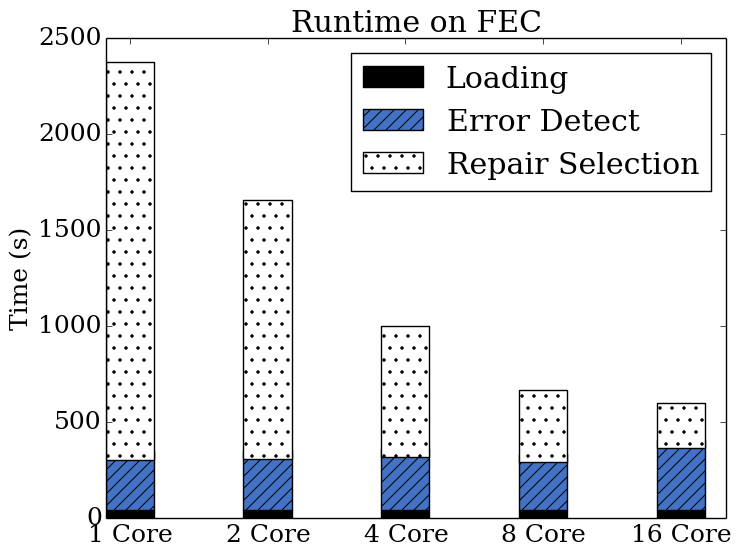
\includegraphics[width=0.8\columnwidth]{exp/runtime.png}
\caption{(A) This plot measures the run-time on a 6M record dataset (1.5GB) grouped by the number of cores on the machine. The repair selection scales but the other steps are not parallelized.\label{exp:runtime}}
\end{figure}

\begin{figure}[t]
\centering
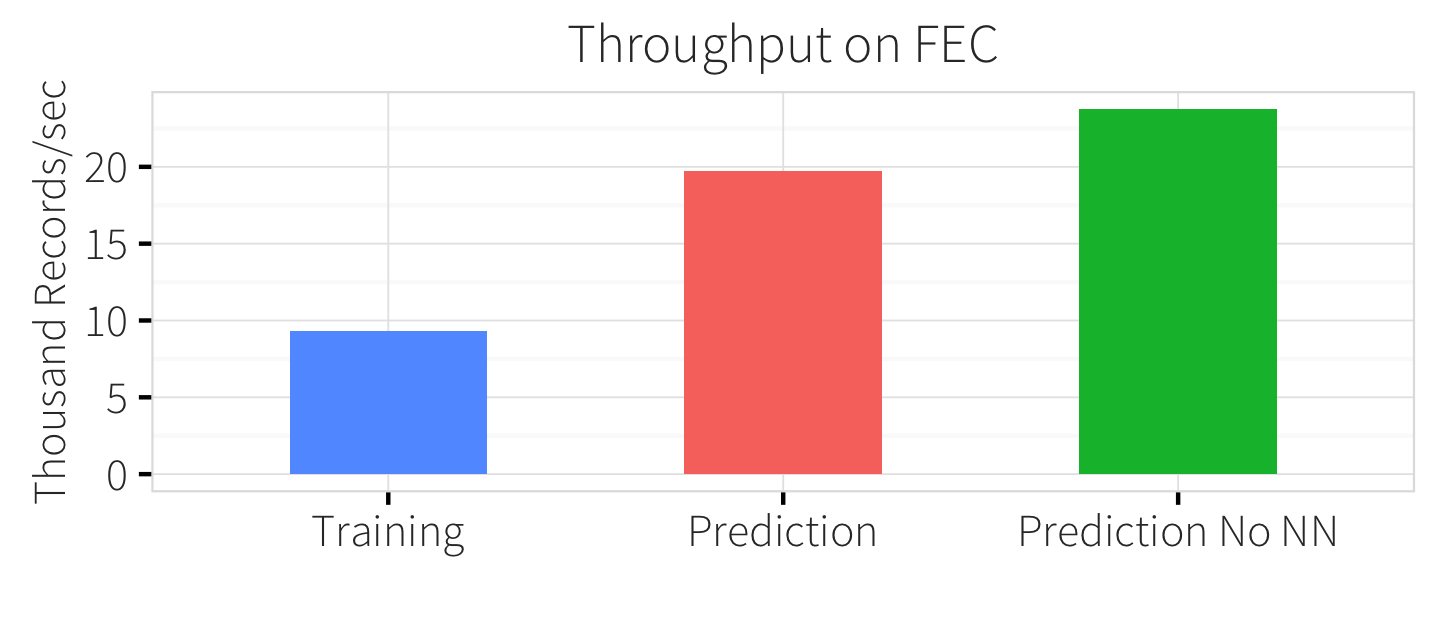
\includegraphics[width=0.8\columnwidth]{exp/runtime2.png}
\caption{We plot the prediction and training throughput for 16-cores. Prediction throughput is much higher than training throughput.\label{exp:tp}}
\end{figure}

\subsection{End-to-End Run Time}
Next, we evaluate the end-to-end wall clock runtime of \sys. We use the FEC dataset since it is the largest. This evaluation includes all of the optimizations for \sys. The FEC dataset is 1.5 GB (about 6M records). 
Figure \ref{exp:runtime} plots the results.
With a single core, \sys takes 2422 seconds in wall-clock time. Of that time, 2072 seconds is spent in repair selection, 306 seconds is spent in error detection, and 44 seconds in loading the dataset.
We can parallelize the repair selection step. We parallelize the inner-loop of the boosting algorithm. On 16-cores, we are able to reduce the runtime of the repair selection to 212 seconds. This constitutes a 9.7x speedup for that step.

It is important to note that this latency is only incurred during training. During prediction, the learned model can be applied, and this process is much faster than training. 
Figure \ref{exp:tp} plots the throughput of \sys.
The number of records that can be processed per second on 16 cores for prediction is 19746 records/second, but during training it is 9316 records/second. One of the key bottlenecks is evaluating the word2vec model for each prediction, and without this model, the throughput increases to 23746 records/second.

\begin{figure}[t]
\centering
 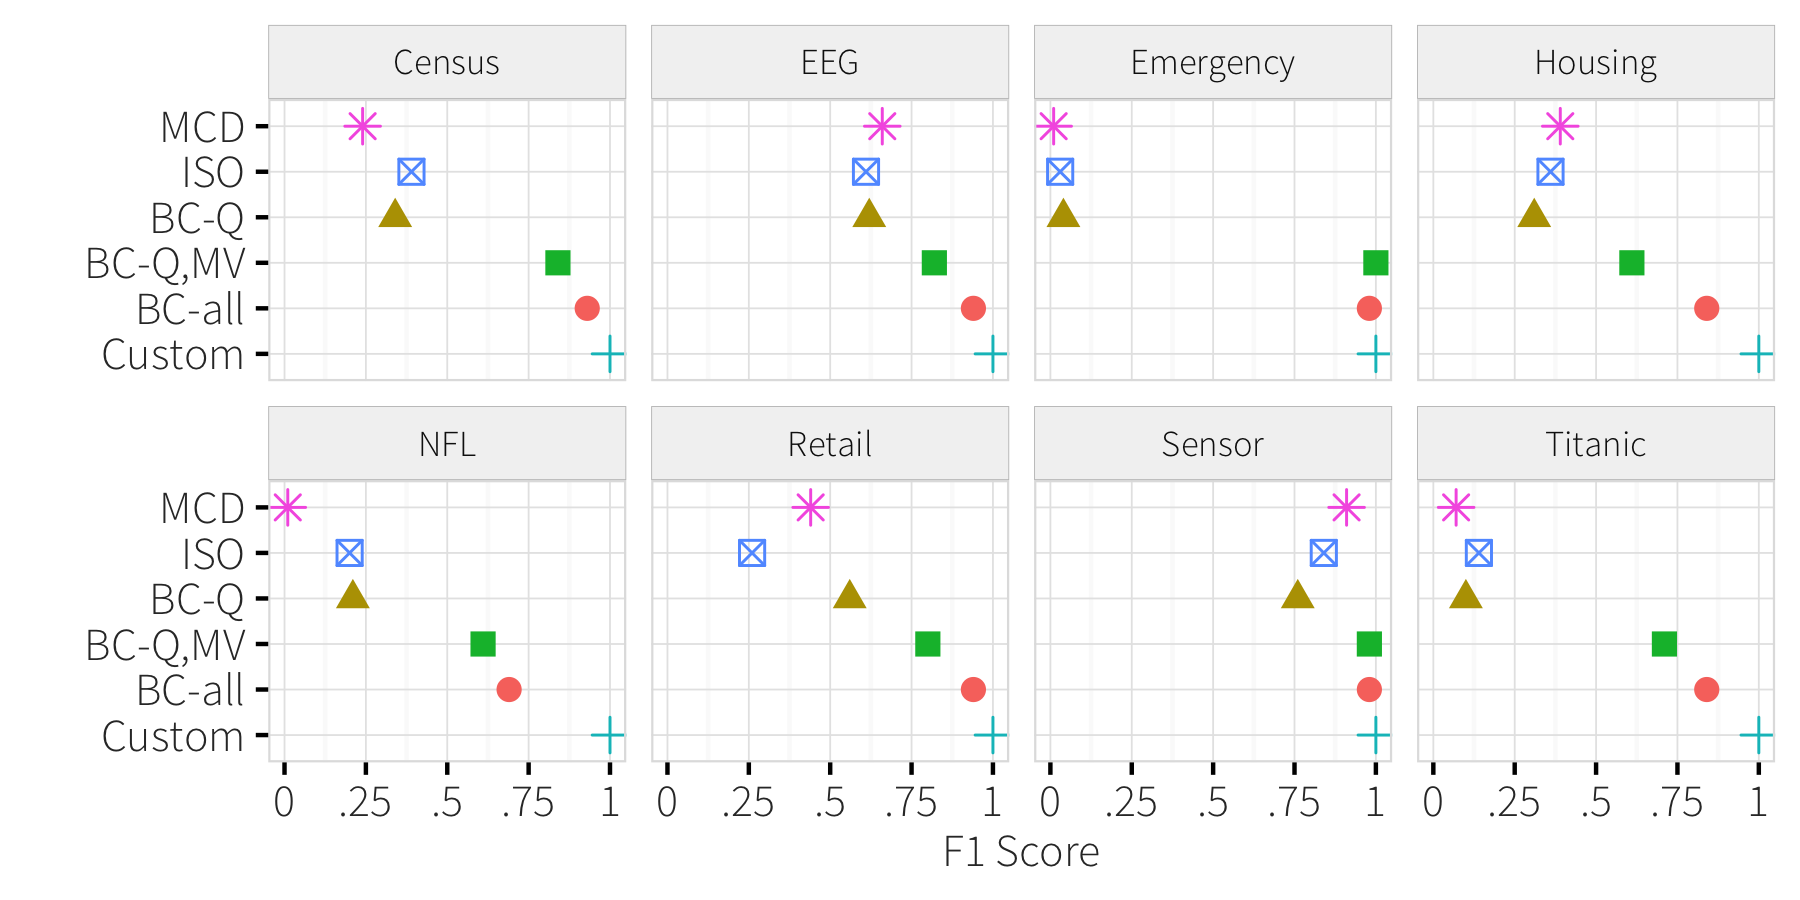
\includegraphics[width=\columnwidth]{exp/daccuracy.png}
 \caption{On 8 Machine Learning competition datasets, we evaluated the F1 accuracy score of different error detection techniques. We compare against Isolation Forest (alone), Minimum Covariance Determinants, and Hand-Written rules. We evaluate \sys using only the Isolation forest for numerical outliers, outliers+missing values, and outliers+missing values+word2vec.
 The final detector in \sys achieves up to 81\% of the accuracy on the competition datasets.
 \label{fig:derror}}
\end{figure}

\begin{figure}[t]
\centering
 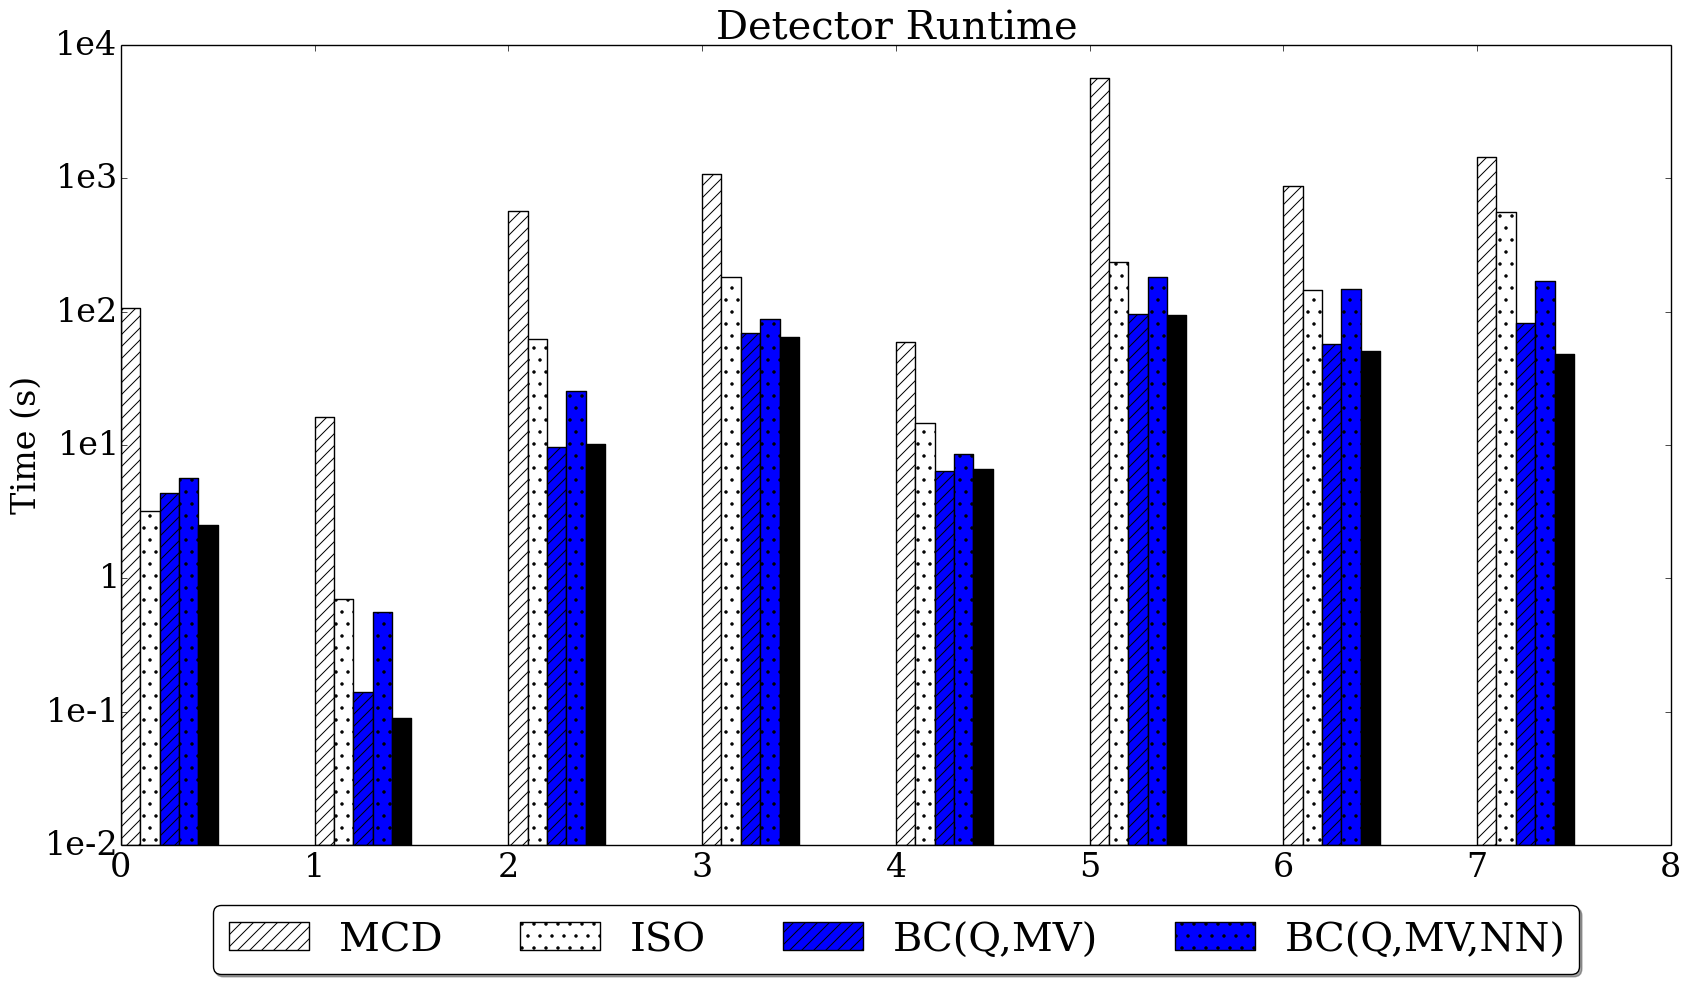
\includegraphics[width=\columnwidth]{exp/druntime.png}
 \caption{On 8 Machine Learning competition datasets, we evaluated the runtime of each of the detection methods. We compare against Isolation Forest, Minimum Covariance Determinants, and Hand-Written rules. While evaluating hand-written rules is certainly faster, \sys is faster in terms of wall-clock time than MCD.
 \label{fig:druntime}}
\end{figure}

\subsection{Micro-Benchmarks}
Next, we evaluate the different components of \sys in terms of accuracy and runtime.

\subsubsection{Detectors}
The first component that we evaluate are the detectors. We design a set of automatic error detectors based on heuristics, statistical criteria, and the word2vec neural network. We first measure its accuracy against hand-written detection scripts, and other quantitative outlier detection techniques (Isolation Forests and Minimum Covariance Determinants).
\sys internally uses an Isolation Forest combined with other error detectors, so we evaluate \sys with and without certain detection modules.
We measure accuracy w.r.t the alternatives with the F1 accuracy measure.

 Figure  \ref{fig:derror} shows that the final detector in \sys achieves up to 81\% of the accuracy of hand-written rules on the competition datasets.
Confirming the results of Abedjan et al.~\cite{DBLP:journals/pvldb/AbedjanCDFIOPST16}, we found that a 
purely quantitative approach does not perform well in comparison to the rule-based approach on these datasets (Isolation Forest alone and MCD).
However, results are significantly improved when combined with heuristics that detect missing values. 
The performance gap is even further reduced when the detector additionally uses a Neural Network to learn how attributes correlate with each other, and detect anomolous correlations.
It is important to emphasize that these datasets represent a very specific domain, i.e., structured training datasets for ML.
The datasets are already in a structured schema and the only thing that an analyst has to worry about is handling inconsistent attribute values.
Presumably these datasets were also previously cleaned and extracted before they were publicly released.
Our initial experiment showed that for this class of datasets, reasonably accurate error detection is possible with minimal supervision and tuning.

 Figure  \ref{fig:druntime} shows the runtime of each of the approaches.
 We found that MCD was a very expensive quantitative error detection approach (orders of magnitude slower).
 This was one of the big motivations for using an isolation forest internally in \sys.
 Of course, rules are faster to evaluate than a learning detector and this gap was on average a factor of 3.
 
 \begin{figure}[t]
\centering
 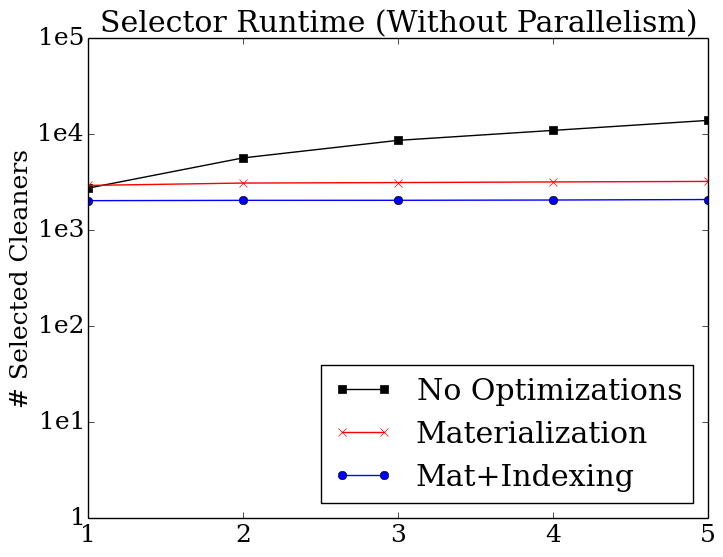
\includegraphics[width=0.8\columnwidth]{exp/opt1.png}
 \caption{This plot (log scale) shows the impact of optimizations on the selector's runtime. Materialization and Indexing allow the algorithm to scale with the number of selected cleaners. Otherwise, the algorithm repeatedly retrains and recleans the same data.
 \label{fig:opt}}
\end{figure}
 
 \subsubsection{Repair Selector Optimizations}
 Next, we evaluate the selector optimizations. We proposed two systems optimizations to the boosting algorithm: (1) materialization, and (2) indexing.
 In this set of experiments, we use FEC dataset and apply no parallelism.
 Figure \ref{fig:opt} plots the runtime of the repair selector as a function of the number of cleaners to select (i.e., B).
 Without any optimization, for $B=1$ the repair selector requires 2754 seconds and for $B=5$ requires 14002 seconds.
 The materialization optimization allows us to pay an up-front cost of creating the view during the first iteration of the algorithm, but saves effort on future iterations.
 For $B=1$ with the materialization optimization, the run time is 2943 seconds.
 For $B=5$ the time is drastically cut down to 3241 seconds.
 In each iteration, the indexing algorithm allows us to more efficiently evaluate the accuracy of a cleaner+classifier pair.
 This reduces the run time at $B=5$ to 2072.
 
 \begin{figure}[t]
\centering
 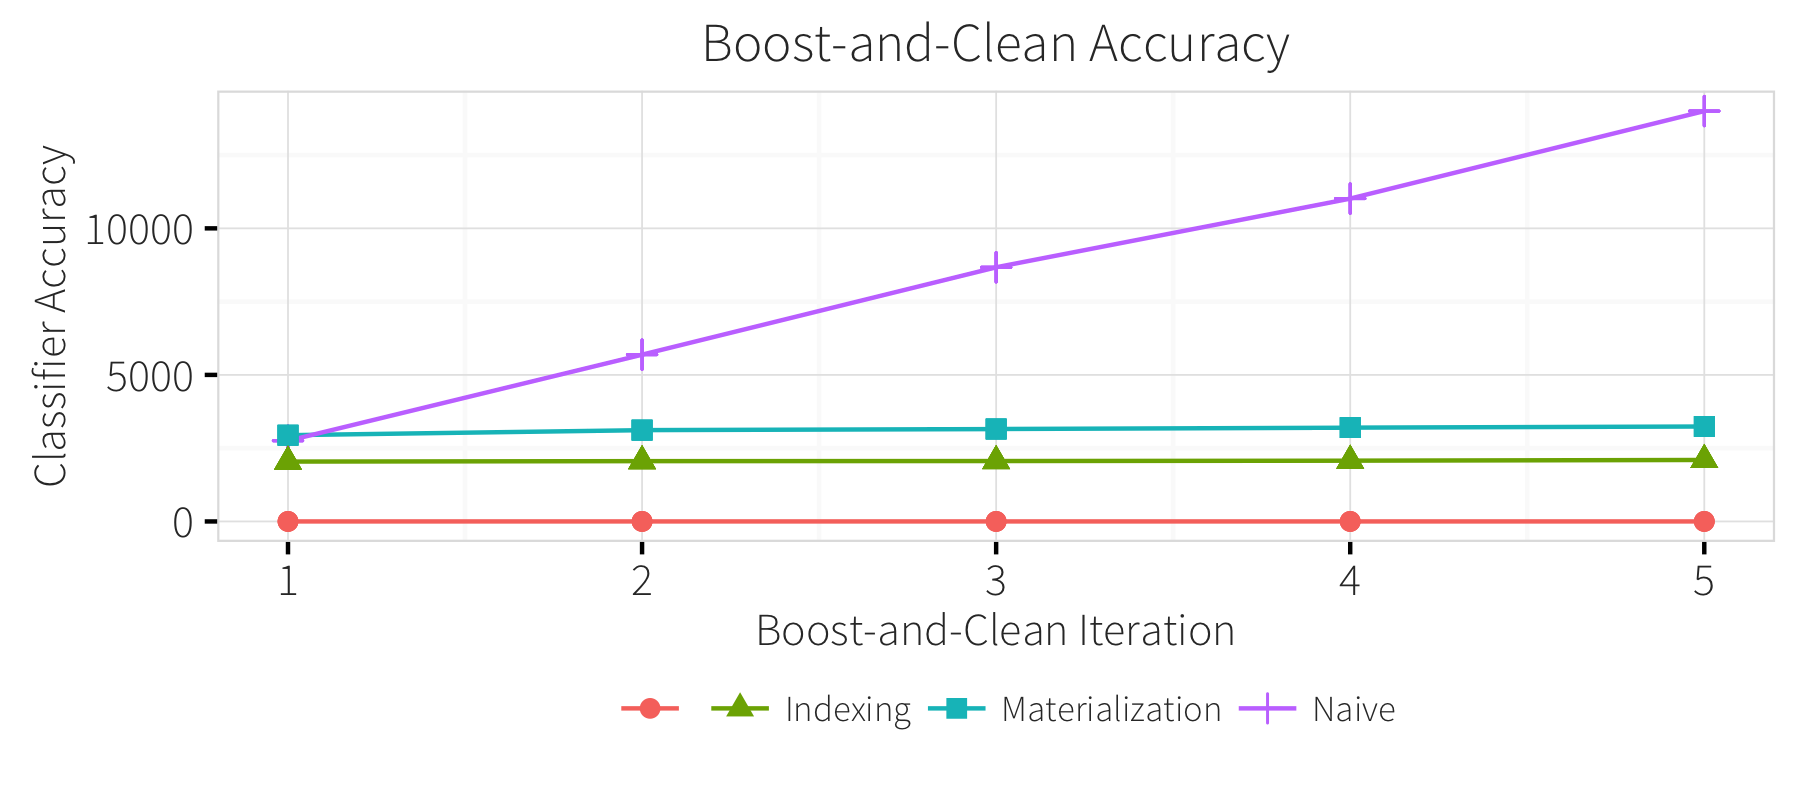
\includegraphics[width=0.8\columnwidth]{exp/learn.png}
 \caption{For three different classification models, we plot the learning curves for the repair selector. Selecting too many cleaners can lead to overfitting.
 \label{fig:learning}}
\end{figure}
 
 \subsubsection{Repair Selector Overfitting}
 One concern with the repair selector is overfitting. We evaluate to what extent, \sys overfits in Figure \ref{fig:learning}, where we plot the learning curves (accuracy as a function of the number of cleaners $B$).
 We try three different classification models, random forests, SVMs, and logistic regression.
 For all of the models we see similar results, where there is an optimal $B$ to select after which \sys overfits.
This is a major concern on small datasets \ewu{How Small?}, but for a sufficiently large dataset with proper test and training evaluation, this can be set through cross-validation. 

\subsubsection{Synthetic Corruptions}

 



%\section{Conclusion and Future Work}
We have shown that automated data cleaning for predictive models can be cast in a statistical boosting framework.  We have prototyped this idea in \sys, a new data cleaning system that detects errors in ML data and uses knowledge of the labels to adaptively select from a set of repair actions to maximize prediction accuracy.
We evaluated results on 8 ML datasets on Kaggle and the UCI repository with real data errors and compare to statistical anomaly detection techniques, constraint-based techniques, and the best single cleaner performance. In all 8 datasets, \sys increased the  test accuracy over alternatives. In addition, we evaluated \sys on production datasets from a data science company and showed that, despite high class imbalances in both datasets, \sys can automatically detect data errors and improve the AUC of the downstream model by $8-9\%$.  We also demonstrate how our optimizations can achieve an end-to-end speed up of over $22\times$

%can parallelize the inner-loop of the boosting operation, and on a 16-core machine \sys achieves a 9.7x speedup. Similarly, we show that building an inverted index can speed up operator selection time by 2.3x.

We are excited about these promising results and have identified a number of future research directions to improve the practicality of the system.  The first is to relax the current requirements of having a test set with clean labels.   Although it may be difficult to acquire sufficient test labels, data science application often have access to an indirect model accuracy measure.  For instance, user retention may be strongly correlated to model accuracy and much easier to obtain.  This will likely require a more complex ensembling technique than boosting.  A second direction is to support parameterized cleaning operations, such as regular expression extractors, for which the number of possible parameter values is unbounded.  We believe that recursive discretization procedures are a promising approach.  A third direction are further performance optimizations so that \sys can scale to large and heterogeneous settings such as data lakes.  Finally, we are actively seeking to continue industrial collaborations and real-world evaluations of our system.  The system and code is open source and can be accessed at {\bf anonymized for submission.}



%\bibliographystyle{abbrv}
%\scriptsize
%\fontsize{8.8pt}{9.9pt} \selectfont
\bibliographystyle{abbrv}
\bibliography{ref} 
\normalsize \selectfont
%\appendix
%
\vspace{0.5em}\noindent\textbf{USCensus: } This dataset contains US Census records for adults and the goal is to predict  whether the adult earns more than $50,000$ dollars. It contains 32,561 records with 15 numerical and categorical attributes. This dataset contained missing values and coding inconsistencies.
Examples of data error include:
\begin{lstlisting}
#missing values
40,Private,121772,Assoc-voc,11,
Married-civ-spouse,Craft-repair,Husband, 
Asian-Pac-Islander,Male,0,0,40,(*\orange{\bf{?}}*),>50K

#coding inconsistency
57,Local-gov,110417,HS-grad,9,
Married-civ-spouse,Craft-repair,Husband,
White,Male,(*\orange{\bf{99999}}*),0,40,United-States,>50K
\end{lstlisting}


\vspace{0.5em}\noindent\textbf{NFL: } This dataset contains play-by-play logs from US Football games. The dataset contains 46,129 records with 65 numerical, categorical, and string-valued attributes. Given the record, the classification objective is to determine whether the next play the team runs is a run or a pass play.
The dataset contains a significant number of missing values and ``sentinel'' records that mark the end of a log sequence. The sentinel records do not signify a play but rather signify a timeout, end of quarter, or end of the game.
\begin{lstlisting}
#missing values
"36",2015-09-10,"2015091000",1,1,(*\orange{\bf{NA}}*),"15:00",
15,3600,0,"NE",35,35,0,0,0,(*\orange{\bf{NA}}*),"PIT","NE"(*\blue{\bf{....}}*)

#sentinel record
"189710",2016-01-03,"2016010310",10,2,NA,"00:00",
0,1800,8,"GB",17,17,0,-1,0,0,"",NA,"END(*~*)QUARTER2"
,1,0,0,0,NA, NA,NA,0,"Quarter(*~*)End"(*\blue{\bf{....}}*)
\end{lstlisting}


\vspace{0.5em}\noindent\textbf{EEG: } This is a dataset of EEG recordings. 
The training data is organized into ten minute EEG clips labeled "Preictal" for pre-seizure data segments, or "Interictal" for non-seizure data segments. 
There are 2406 records each of which is a variable-length time-series of 16 attributes. We featurize this dataset into records of 32 attributes--the mean and variance over the length of the time-series. 
This dataset primarily contains numerical outliers, the clips have spurious readings.
\begin{lstlisting}
#Time t=46 Normal
[-41.53080368041992, -9.605541229248047, 
-55.74542999267578, 17.77084732055664,
-1.6866581439971924, 38.86453628540039, 
17.108707427978516, 26.545927047729492, 
-12.696817398071289, -12.703478813171387, 
56.78707504272461, 3.2556533813476562, 
22.688213348388672, -25.728403091430664, 
-10.142332077026367, -11.585281372070312]

#Time t=47 Abnormal
(*\orange{[0, 8, -10, 9, 18, 6, -8, -41, -26, -72, -19, 70, 129, 53, 31, -11]}*)
\end{lstlisting}

\vspace{0.5em}\noindent\textbf{Sensor: } The Intel sensor dataset contains 928,991 temperature, humidity, and light sensor readings a sensor deployment. The classification task is to predict whether the readings came from a particular sensor (sensor 49). This dataset primarily has numerical outliers.
\begin{lstlisting}
#Normal Record
49  -0.999750  12.862100  10.368300  10.438300  
11.669900 (*\orange{\bf{13.493100}}*)  13.342300  8.041690  
8.739010  26.225700  59.052800

#Spurious Record
49  1.175188  12.279100  8.849360  9.005830  
10.111700  (*\orange{\bf{378.750000}}*)  19.319400  15.916200  
37.631400  27.150100  53.403700
\end{lstlisting}

\vspace{0.5em}\noindent\textbf{Titanic: } This dataset contains 891 records from the Titanic manifest with 12 attributes. The classification objective is to determine whether the passenger survived or not. There are missing values and string formatting errors.

\begin{lstlisting}
#missing values
891,0,3,"Dooley, Mr. Patrick",male,
32,0,0,370376,7.75,(*\orange{\bf{--}}*),Q
\end{lstlisting}

\vspace{0.5em}\noindent\textbf{Housing: } The housing dataset contains 1460 records and 81 attributes of house price listings. The classification objective is to determine whether the listed house will be sold above 750000. 
This dataset contains missing values as well as numerical outliers.
\begin{lstlisting}
#missing values
(*\blue{\bf{....}}*)204,228,0,0,0,(*\orange{\bf{NA,NA}}*),Shed,350,11,2009,WD,
Normal,200000
\end{lstlisting}

\vspace{0.5em}\noindent\textbf{Retail: } The online retail dataset contains 541,909 records of online retail purchases with 8 attributes. The classification objective is to predict whether the purchase occurred in the United Kingdom.
This dataset contains numerical errors where some purchased quantities are reported as negative.

\begin{lstlisting}
#outliers
C536391,21980,PACK OF 12 RED RETROSPOT TISSUES
,(*\orange{\bf{-24}}*),12/1/10 10:24,0.29,17548,United Kingdom
\end{lstlisting}

\vspace{0.5em}\noindent\textbf{Federal Election Commission Contributions: } The FEC provides a dataset of election contributions of 6,410,678 records with 18 numerical, categorical and string valued attributes. This dataset has a number of errors. There are missing values, formatting issues (where records have the wrong number of fields causing misaligment in parsing), and numerical outliers (negative contributions).

\begin{lstlisting}
#missing values
C00458844,"P60006723","Rubio, Marco","RUCINSKI,
ROBERT","APO","AE","090960009","US ARMY",
"PHYSICIAN",100,08-MAR-16,(*\orange{\bf{``''}}*),(*\orange{\bf{``''}}*),(*\orange{\bf{``''}}*),"SA17A",
"1082559","SA17.1074981","P2016"

#rejected contributions double recorded
C00458844,"P60006723","Rubio, Marco","SWAID, 
SWAID N. DR.","BIRMINGHAM","AL","352660827",
"NEWOLOGICAL SURGERY ASSOCIATES","PHYSICIAN",
(*\orange{\bf{-400}}*),28-DEC-15, "REDESIGNATION TO GENERAL","X",
"REDESIGNATION TO GENERAL","SA17A",
"1047126","SA17.892835B","P2016"
\end{lstlisting}

\vspace{0.5em}\noindent\textbf{Restaurant Dataset: } The restaurant dataset has 758 distinct records and 4 attributes. This dataset has typically been used as a benchmark for entity resolution since records are duplicated with minor inconsistencies.
We designed a multi-class classification task to see if we could predict the city from record.
One of the major inconsistencies was additional attributes appended to the restaurant category.

\begin{lstlisting}
campanile,624 s. la brea ave.,los angeles,
american

grill  the,9560 dayton way,beverly hills,
american (*\orange{\bf{(traditional)}}*)
\end{lstlisting}


\vspace{0.5em}\noindent\textbf{Housing: } The housing dataset contains 1460 records and 81 attributes of house price listings. The classification objective is to determine whether the listed house will be sold above 750000. 
This dataset contains missing values as well as numerical outliers.

\begin{lstlisting}
#missing values
(*\blue{\bf{....}}*)204,228,0,0,0,(*\orange{\bf{NA,NA}}*),Shed,350,11,2009,WD,
Normal,200000
\end{lstlisting}

\end{document}
